% This is based on the LLNCS.DEM the demonstration file of
% the LaTeX macro package from Springer-Verlag
% for Lecture Notes in Computer Science,
% version 2.4 for LaTeX2e as of 16. April 2010
%
% See http://www.springer.com/computer/lncs/lncs+authors?SGWID=0-40209-0-0-0
% for the full guidelines.
%

\documentclass{llncs}
\usepackage{listings}
\usepackage{amsmath}
\usepackage{longtable}
\usepackage{booktabs}
\usepackage{graphicx}

\providecommand{\tightlist}{%
  \setlength{\itemsep}{0pt}\setlength{\parskip}{0pt}}

\begin{document}

\title{Project Documentation for Open Environmental Data Cloud Prototyping Project}
%
\titlerunning{Open Data}  % abbreviated title (for running head)
%                                     also used for the TOC unless
%                                     \toctitle is used
%
\author{Andres Ardila, Rohullah Ayobi, Oliver Bruski, Ahmad Jawid Jami, Amer Jazaerli, Nico Tasche, Paul Wille}

\institute{Technische Universit\"at Berlin, Stra\ss{}e des 17. Juni 135, 10623 Berlin, Germany,\\
\email{nico.tasche@campus.tu-berlin.de}}

\maketitle              % typeset the title of the contribution

\begin{abstract}
\keywords{Open Data, Environemental Data, Big Data}
\end{abstract}

\pagebreak

\tableofcontents

\clearpage

%%%%%%%%%%%%%%%%%%%%%%%
%% Content %%%%%%%%%%%%
%%%%%%%%%%%%%%%%%%%%%%%

\section{Data Source Metadata Management System}\label{sec:metadata}

\textbf{Authoriship: } Written by Paul Wille\\
\emph{Proofread \& edited by Andres} \\

\vspace*{4mm}

In this chapter we will discuss the component responsible for managing
metadata about the data sources which are imported to the system. We
will cover what it is and does, some thoughts around why we decided to
include such a component, and how it was realized and implemented.

\subsection{Requirements}\label{requirements}

The main purpose of the component is to:

\begin{itemize}
\tightlist
\item
  serve as a registry of data sources in the system,
\item
  provide data source metadata to other components in the system,
\item
  provide users with information about units of measurement,
\item
  enable users who want to use the data to see the resources our system
  contains
\end{itemize}

In contrast to nearly every other component we had to implement, the
management platform did not have to meet as many criteria as a
distributed cloud system in general. The data it contains is quite
static and the number of requests that we expect is also quite low.
However, the following general cloud-specific architectural style
requirements were taken into consideration:

\begin{itemize}
\tightlist
\item
  Availability to other system components, that require the held
  information
\item
  Quick response time (for query optimization within the public search
  API)
\item
  Ability to run asynchronous background tasks (for scheduling)
\end{itemize}

\subsection{Implementation}\label{implementation}

The system was built using \emph{Ruby on Rails} with \emph{PostgreSQL}
as a database. The reasons why we chose to use Rails are:

\begin{itemize}
\tightlist
\item
  Relatively fast development of an MVC web application
\item
  Well established (over a decade), has therefore lots of resources ---
  also for all kinds of extensions
\item
  Extensive community support
\item
  Very good integrated ORM adapters that could easily be exchanged for
  ODM adapters for document databases
\item
  Offers the dynamic of Ruby as programming language
\end{itemize}

\subsection{Domain Model}\label{domain-model}

\begin{figure}
	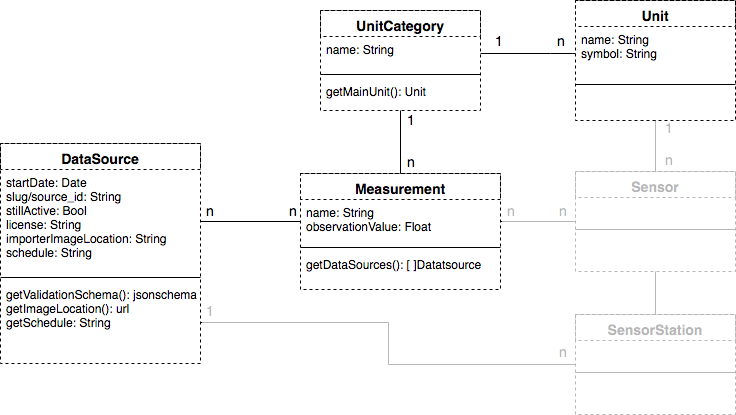
\includegraphics[width=1.00\textwidth]{images/relational_schema.png}
	\caption{UML Class Diagram of the Metadata Management System}
	\label{fig:uml-model}
\end{figure}

\subsubsection{Data Sources Registry}\label{data-sources-registry}

Before data from a given source can be imported, important information
about the source must be made available to our system. This information
consists of static metainformation and has no direct relation to actual
data being provided in the source.

We chose not to store it in the same database as the actual sensor
measurement data, but have a separate system instead. This provides
isolation between our sources and the database, preventing changes in
the choice of database or its schema from having any effect in how we
store and maintain data sources.

The metainformation that has to be provided to our system prior to
importing mainly consists of:

\begin{itemize}
\tightlist
\item
  Name of the source
\item
  Start date from which the source provides data
\item
  Whether the source is still active (i.e.~data is actively being
  provided by the source).
\item
  if not, the end date (last date for which data was provided).
\item
  Under what license the data is published
\end{itemize}

Additionally we ask the user to provide additional information, which is
useful for our system:

\begin{itemize}
\tightlist
\item
  If the data source is still active, at what schedule is new data
  published
\item
  A \emph{slug} that can be used as an id within our pipeline and in
  Elasticsearch
\item
  The measurements provided by the data source (which actual
  measurements the data source collects)
\item
  The URL location of the Docker container to be executed to import the
  data.
\end{itemize}

\begin{figure}
	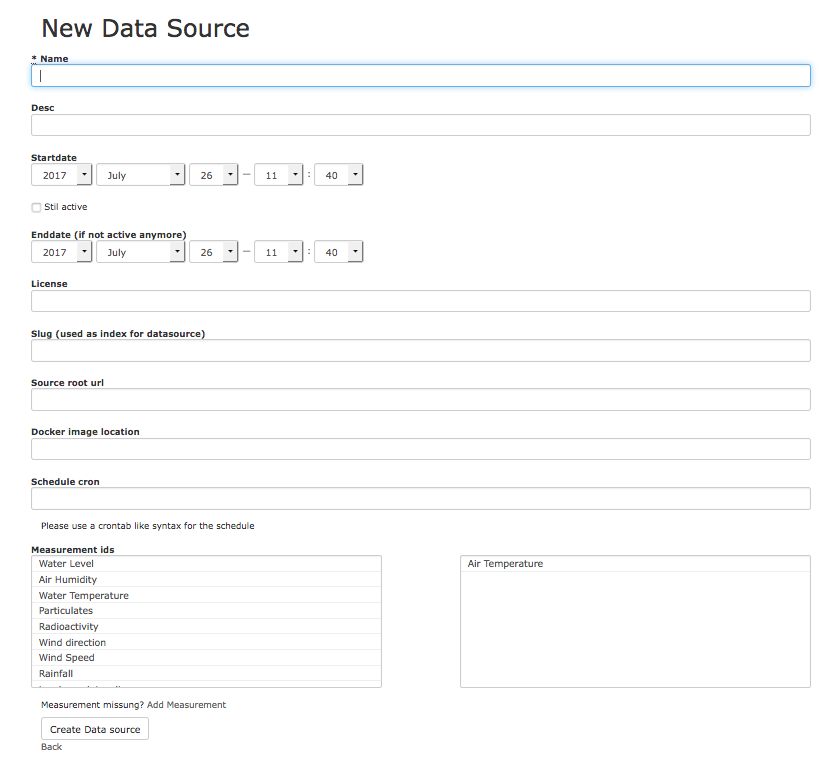
\includegraphics[width=1.00\textwidth]{images/new_datasource.png}
	\caption{Registering a data source within the Web management platform}
	\label{fig:register-source}
\end{figure}

\subsubsection{Validation Schema}\label{validation-schema}

As described in the chapter about validation and insertion into
Elasticsearch, we have a separate, distinct component that is
responsible for validating the output from data importers.

To achieve this, a schema must be provided against which to validate.
Since this schema itself is fixed, it could be hardcoded into the
validator, without the need to make another HTTP request. We decided
that this would be a bad idea for the following reasons:

\begin{itemize}
\tightlist
\item
  Sanity checks: in addition to schema-only validation, the schema
  provided by this component can validate data-source-specific values
  (such as importer IDs, etc.), which could not be validated with a
  generic validator.
\item
  Version management: schema changes over time would require changing
  the information hardcoded within the validator, and completely
  rebuilding and redeploying the validator component itself. Updating a
  record inside this component is far simpler than redeploying
  infrastructure, which is inherently more complex in an era where no
  downtime is expected.
\end{itemize}

Therefore we needed a place where said validation schema can reside. The
web management system seemed to be the right pace for that, as it
already carries metainformation about data sources and the data sources
are registered there. So it is easy to provide the relevant schema
information as well. The management system provides an API call to
supply the validation schema to the validators which looks like this:

\begin{verbatim}
GET /data_sources/:id/getValidationSchema
\end{verbatim}

The response looks like as follows (note that the const
\texttt{source\_id} would be replaced by the ID of the data source):

\begin{verbatim}
{
  "\$schema": "http://json-schema.org/schema#",
  "title": "Data Source",
  "description": "A Data Source for Open Sensor Data from the CP project \\
									at TU Berlin. ",
  "type": "object",
  "properties": {
    "source_id": {"const": "source_slug"},
    "device": {"type": "string"},
    "timestamp": { "type": "string", "format": "date-time" },
    "timestamp_data": { "type": "string", "format": "date-time" },
    "location": {
      "type": "object",
      "properties": {
        "lat": {"type": "number",
                "exclusiveMaximum": true,
                "exclusiveMinimum": true,
                "maximum": 90,
                "minimum": -90
               },
        "lon": {"type": "number",
                "exclusiveMaximum": true,
                "exclusiveMinimum": true,
                "maximum": 180,
                "minimum": -180,
               }
      },
    "required": ["lat", "lon"]
    },
    "license": {"type": "string"},
    "sensors": {
      "type": "object",
      "items": [
      {
        "type": "object",
        "properties": {
          "sensor": {"type": "string"},
          "observation_type": {"type": "string"},
          "observation_value": {"type": "number"}
        }
      }]
    }
  },
  "required": ["source_id", "timestamp","sensors", "location", "license"]
}
\end{verbatim}

\subsubsection{Provide Information to the Elasticsearch API for query
optimization}\label{provide-information-to-the-elasticsearch-api-for-query-optimization}

As described in the data model section, our model is data-source-based
and not measurand-based. For queries spanning across measurands, it will
be necessary to have further information about the relationship between
data sources and measurands.

As there were several possibilities as to where this information could
be stored and managed, and how it would be provided, the easiest place
to start with in our opinion was with the implementer of an importer,
since he or she must provide information to us when registering the data
source. The user therefore has to mark what measurements a data source
contains upfront (see Figure \ref{fig:register-source}).

In order to optimize querying, this information is provided to the API
that wraps the search interface of Elasticsearch via an API itself. The
information is stored in an indexed join table that holds the mapping
between data source and the measurands it contains. As can be seen in
the class diagram \ref{fig:uml-model} of the relational system, queries
in both directions are provided: getting all measurands for a data
source, and getting all data sources that contain a given measurand. The
corresponding routes look like this:

\begin{verbatim}
GET /data_sources/:id/measurements
\end{verbatim}

Example:

\begin{verbatim}
GET /data_sources/blume_messnetz/measurands

[
   {
      "id":1,
      "name":"Air Temperature",
      "desc":"",
      "unit_category_id":"temperature"
   },
   {
      "id":3,
      "name":"Air Humidity",
      "desc":"amount of water vapor present in the air",
      "unit_category_id":"humidity"
   }
]
\end{verbatim}

\begin{verbatim}
GET /measurements/:id/data_sources
\end{verbatim}

An example request would look like following

\begin{verbatim}
GET /measurements/1/data_sources

[
    { "id":1, "slug":"blume_messnetz", "license":"" },
    { "id":5, "slug":"german_weather_service", "license":"" }
]
\end{verbatim}

\subsubsection{Provide configuration information to the deployment
component}\label{provide-configuration-information-to-the-deployment-component}

Since the importer registration the only step in which the implementer
has to provide information to our system, it should cover all
configuration information needed to get an importer running.

\subsubsection{Units}\label{units}

With the requirements in mind, we modeled units like so:

\begin{enumerate}
\def\labelenumi{\arabic{enumi}.}
\tightlist
\item
  \textbf{Unit Categories}: Units themselves belong to a unit category.
  The unit category describes an entity for which measurements exist,
  which express their observations with one of the units of that
  category (see Figure \ref{fig:uml-model}).
\item
  Each unit has a \textbf{main unit} that we decide on. By calling the
  API or visiting the management platform a user can see, which the main
  unit is. Within our datastore we only use the main unit of a unit
  category for expressing measurements.
\item
  Units are managed by admins receptively users with permit to do so.
\item
  We therefore have a curated list of the unit categories and units
\item
  If there are units, measurements or even categories missing, each user
  can propose new ones. This proposals are also managed by the group of
  people managing the units.
\end{enumerate}

Measurements are controlled on the platform itself to allow users to
better propose new measurements, as this may happen more often. Units
and the Unit categories however are managed in a \emph{.yml} file. The
syntax we used looks like following for one entry:

\begin{verbatim}
From config/constants/units.yml:

pascal:
  id: pressure_pascal
  name: "pascal"
  unit_symbol: "pa"
  unit_category_id: pressure
  notation: "1 <centerdot>
              <mfrac>
                <mrow>
                  kg
                </mrow>
                <mrow>
                  m
                  <msup>
                          <mi>s</mi>
                          <mn>2</mn>
                </mrow>
              </mfrac>"

From config/constants/unit_categories.yml:

pressure:
  id: pressure
  name: Pressure
\end{verbatim}

The unit categories are pretty straightforward. For a unit there are
some more possibilities. Besides declaring the unit symbol, the category
it belongs to, its name you are allowed to use MathML to express what
the meaning of a unit is. This is especially helpful with units that can
be directly converted to each other (Figure \ref{fig:screen-units}).

The API of the web management system also provides calls to a) receive
the main unit of a unit category and to b) get a list of all units there
are for a unit category. Both of these information are of course aswell
accessible from the frontend of the system.

\begin{figure}[b]
	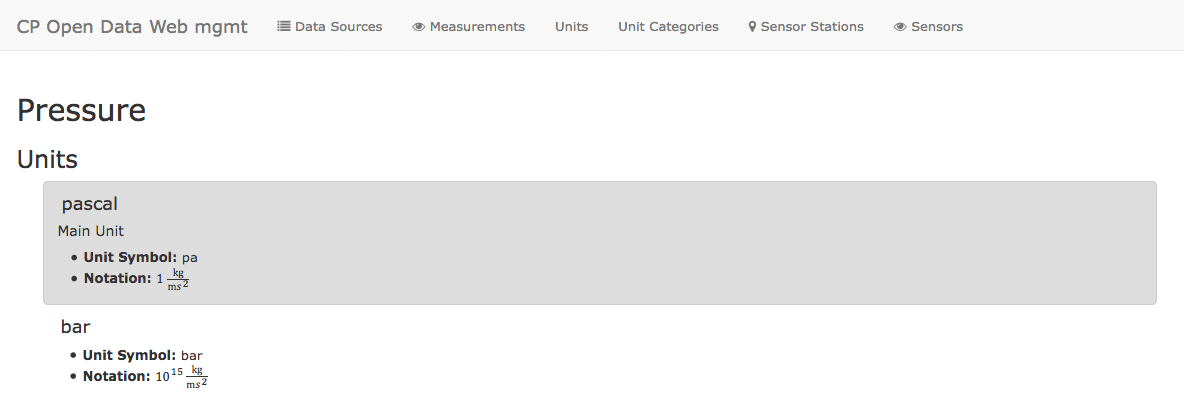
\includegraphics[width=1.00\textwidth]{images/unit_frontend.png}
	\caption{Screenshot of the units of a unit category on the web management platform. You can see the main unit and have a notation on what the units express.}
	\label{fig:screen-units}
\end{figure}

\begin{verbatim}
GET /unit_categories/:id/getMainUnit
\end{verbatim}

Example request:

\begin{verbatim}
GET /unit_categories/temperature/getMainUnit

{
    "id":"temperature_celsius",
    "name":"celsius",
    "unit_category_id":"temperature",
    "unit_symbol":"°C"
}
\end{verbatim}

\begin{verbatim}
GET /unit_categories/:id/units
\end{verbatim}

Example request:

\begin{verbatim}
GET /unit_categories/temperature/units

[
   {
      "attributes":{
         "id":"temperature_celsius",
         "name":"celsius",
         "unit_symbol":"°C",
         "unit_category_id":"temperature",
         "notation":""
      }
   },
   {
      "attributes":{
         "id":"temperature_fahrenheit",
         "name":"fahrenheit",
         "unit_symbol":"°F",
         "unit_category_id":"temperature",
         "notation":""
      }
   },
   {
      "attributes":{
         "id":"temperature_kelvin",
         "name":"kelvin",
         "unit_symbol":"K",
         "unit_category_id":"temperature",
         "notation":""
      }
   },
   ...
]
\end{verbatim}

\subsection{Discussion}\label{discussion}

As mentioned before, the planning of the extent of the functionality
offered by this system, was very vague. Besides managing metadata and
providing an API for other components, further features were at least
considered to be part of this system, like for example a scheduler that
triggers the component that handles the deployment of importers.
Therefore we chose to build this system on top of an infrastructure that
can be easily extended in many directions and has nice-to-use database
adapters instead of a more lightweight system.

While initially we also wanted to model a data source with its sensors
grouped in sensor stations, this approach would bring immense overhead
for configuring data sources in our system upfront, as a user would have
to very exactly model a data source with all its sensors and sensor
stations first. For big services like e.g.~the German Weather Service
this would be an enormous amount of work. Gathering this information
would better be done by scraping the information present in
Elasticsearch and translating them to geolocated information for all
sensors/sensor-stations/datasources. In the UML Class Diagram you can
see the modeling for this approach greyed out.

The main metainformation about the data sources (besides metadata about
the source itself) that we still needed within our system (the location
of the sensor and the grouping of sensor stations is not essential for
our system to work) and had to offer to the user registering a source
were then:

\begin{itemize}
\tightlist
\item
  Information about the measurands offered by the data source
\item
  Information about the main unit used for a measurand (see section Unit
  system)
\end{itemize}

\subsubsection{Future Improvements}\label{future-improvements}

\paragraph{Caching}

There is currently no caching solution implemented since the workloads
during development phase were quite manageable. Also including a
distributed caching system in our production pipeline seemed to be too
high of an effort and would take up significant resources that would
actually not be needed during development. We wanted, therefore, to use
the limited and expensive resources we had for actual importing.

As the number of data importers grows in production, however, requests
to the relational database would increase accordingly. Whereas scaling
the database would allow us to avoid the bottleneck, adding a cache in
front of the database to serve read requests would be sufficient to
ensure performance without incurring the cost and added complexity of
scaling. An important consideration, of course, is the frequency with
which data is updated (in our case low to none), thus making it a
perfect candidate for caching. As a distributed caching system where
read requests are very fast and possible on all nodes, Redis would be a
good fit for this use case. Writing is quite expensive due to the
replication method used by Redis, but because of the infrequent updates
to our data, we are willing to accept the trade-off in exchange for very
fast reads.

\paragraph{Exchange Scheduling information}

Due to not quite being able to reach every goal of our initial plan as
to how the architecture should look like, the scheduler had to move to
the deployment component (i.e.~the deployment to the Kubernetes
cluster). While this component should be responsible for deploying data
importers, the information about the schedule should actually be
provided to the web management system by the user. This is currently not
happening. There would be several ways how to manage scheduling and/or
deliver the scheduling information from this system to the component
handling the scheduling.

\begin{itemize}
\tightlist
\item
  Having a background processing component that acts as a scheduler
  within the web management platform. This would require an API to
  trigger the deploy on the component responsible for that, which we
  were not able to achieve.
\item
  Having a microservice-like component that is only responsible for
  scheduling and triggering importers to be deployed. This would as well
  require an API on the deployment component.
\item
  Leave the scheduling within the deployment component. This would also
  require an API, but just for receiving the general schedule, not for
  offering a hook to trigger an import.
\end{itemize}

The second option seems more granular and conforms better to our general
microservice approach but would also require the most configuration and
deployment effort. Including a scheduler in the web management platform
would somehow violate this approach but still make sense, as this
component could easily be integrated within Ruby on Rails and would be a
standalone component within it.

\section{Data Source Metadata Management System}\label{sec:metadata}

\textbf{Authoriship: } Written by Paul Wille\\
\emph{Proofread \& edited by Andres} \\

\vspace*{4mm}

In this chapter we will discuss the component responsible for managing
metadata about the data sources which are imported to the system. We
will cover what it is and does, some thoughts around why we decided to
include such a component, and how it was realized and implemented.

\subsection{Requirements}\label{requirements}

The main purpose of the component is to:

\begin{itemize}
\tightlist
\item
  serve as a registry of data sources in the system,
\item
  provide data source metadata to other components in the system,
\item
  provide users with information about units of measurement,
\item
  enable users who want to use the data to see the resources our system
  contains
\end{itemize}

In contrast to nearly every other component we had to implement, the
management platform did not have to meet as many criteria as a
distributed cloud system in general. The data it contains is quite
static and the number of requests that we expect is also quite low.
However, the following general cloud-specific architectural style
requirements were taken into consideration:

\begin{itemize}
\tightlist
\item
  Availability to other system components, that require the held
  information
\item
  Quick response time (for query optimization within the public search
  API)
\item
  Ability to run asynchronous background tasks (for scheduling)
\end{itemize}

\subsection{Implementation}\label{implementation}

The system was built using \emph{Ruby on Rails} with \emph{PostgreSQL}
as a database. The reasons why we chose to use Rails are:

\begin{itemize}
\tightlist
\item
  Relatively fast development of an MVC web application
\item
  Well established (over a decade), has therefore lots of resources ---
  also for all kinds of extensions
\item
  Extensive community support
\item
  Very good integrated ORM adapters that could easily be exchanged for
  ODM adapters for document databases
\item
  Offers the dynamic of Ruby as programming language
\end{itemize}

\subsection{Domain Model}\label{domain-model}

\begin{figure}
	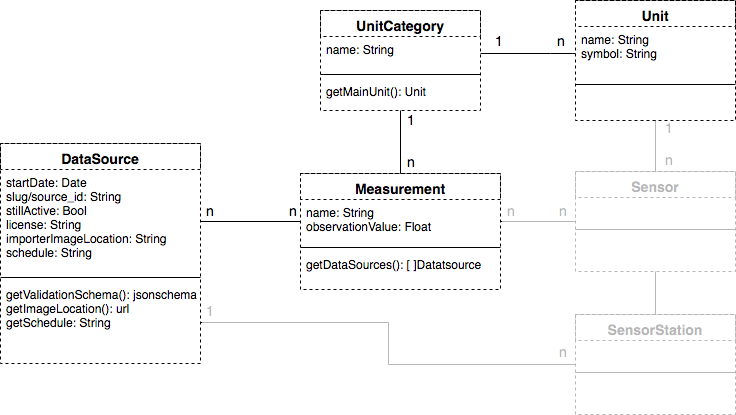
\includegraphics[width=1.00\textwidth]{images/relational_schema.png}
	\caption{UML Class Diagram of the Metadata Management System}
	\label{fig:uml-model}
\end{figure}

\subsubsection{Data Sources Registry}\label{data-sources-registry}

Before data from a given source can be imported, important information
about the source must be made available to our system. This information
consists of static metainformation and has no direct relation to actual
data being provided in the source.

We chose not to store it in the same database as the actual sensor
measurement data, but have a separate system instead. This provides
isolation between our sources and the database, preventing changes in
the choice of database or its schema from having any effect in how we
store and maintain data sources.

The metainformation that has to be provided to our system prior to
importing mainly consists of:

\begin{itemize}
\tightlist
\item
  Name of the source
\item
  Start date from which the source provides data
\item
  Whether the source is still active (i.e.~data is actively being
  provided by the source).
\item
  if not, the end date (last date for which data was provided).
\item
  Under what license the data is published
\end{itemize}

Additionally we ask the user to provide additional information, which is
useful for our system:

\begin{itemize}
\tightlist
\item
  If the data source is still active, at what schedule is new data
  published
\item
  A \emph{slug} that can be used as an id within our pipeline and in
  Elasticsearch
\item
  The measurements provided by the data source (which actual
  measurements the data source collects)
\item
  The URL location of the Docker container to be executed to import the
  data.
\end{itemize}

\begin{figure}
	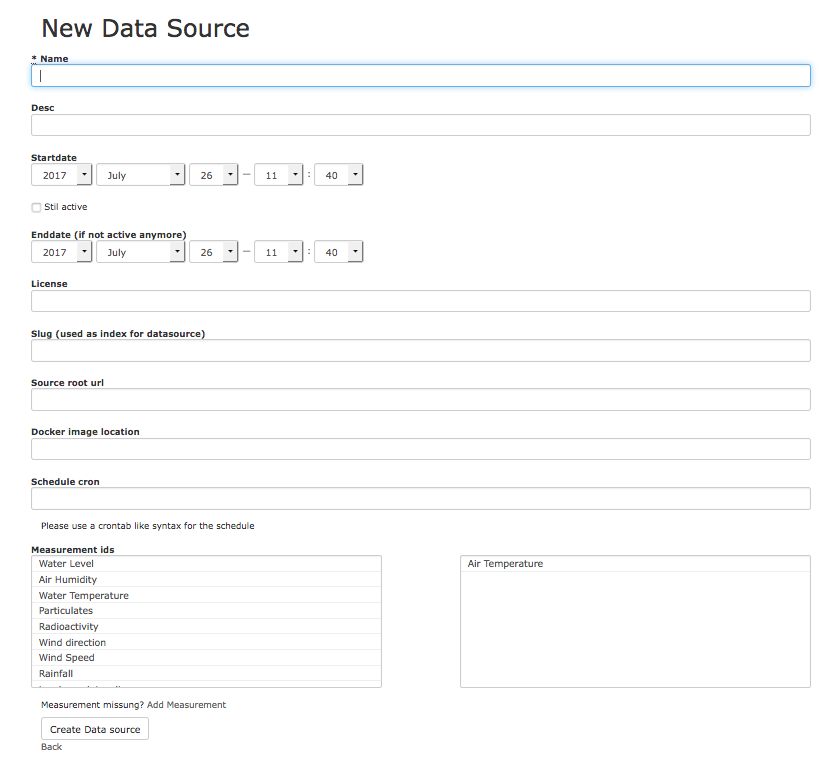
\includegraphics[width=1.00\textwidth]{images/new_datasource.png}
	\caption{Registering a data source within the Web management platform}
	\label{fig:register-source}
\end{figure}

\subsubsection{Validation Schema}\label{validation-schema}

As described in the chapter about validation and insertion into
Elasticsearch, we have a separate, distinct component that is
responsible for validating the output from data importers.

To achieve this, a schema must be provided against which to validate.
Since this schema itself is fixed, it could be hardcoded into the
validator, without the need to make another HTTP request. We decided
that this would be a bad idea for the following reasons:

\begin{itemize}
\tightlist
\item
  Sanity checks: in addition to schema-only validation, the schema
  provided by this component can validate data-source-specific values
  (such as importer IDs, etc.), which could not be validated with a
  generic validator.
\item
  Version management: schema changes over time would require changing
  the information hardcoded within the validator, and completely
  rebuilding and redeploying the validator component itself. Updating a
  record inside this component is far simpler than redeploying
  infrastructure, which is inherently more complex in an era where no
  downtime is expected.
\end{itemize}

Therefore we needed a place where said validation schema can reside. The
web management system seemed to be the right pace for that, as it
already carries metainformation about data sources and the data sources
are registered there. So it is easy to provide the relevant schema
information as well. The management system provides an API call to
supply the validation schema to the validators which looks like this:

\begin{verbatim}
GET /data_sources/:id/getValidationSchema
\end{verbatim}

The response looks like as follows (note that the const
\texttt{source\_id} would be replaced by the ID of the data source):

\begin{verbatim}
{
  "\$schema": "http://json-schema.org/schema#",
  "title": "Data Source",
  "description": "A Data Source for Open Sensor Data from the CP project \\
									at TU Berlin. ",
  "type": "object",
  "properties": {
    "source_id": {"const": "source_slug"},
    "device": {"type": "string"},
    "timestamp": { "type": "string", "format": "date-time" },
    "timestamp_data": { "type": "string", "format": "date-time" },
    "location": {
      "type": "object",
      "properties": {
        "lat": {"type": "number",
                "exclusiveMaximum": true,
                "exclusiveMinimum": true,
                "maximum": 90,
                "minimum": -90
               },
        "lon": {"type": "number",
                "exclusiveMaximum": true,
                "exclusiveMinimum": true,
                "maximum": 180,
                "minimum": -180,
               }
      },
    "required": ["lat", "lon"]
    },
    "license": {"type": "string"},
    "sensors": {
      "type": "object",
      "items": [
      {
        "type": "object",
        "properties": {
          "sensor": {"type": "string"},
          "observation_type": {"type": "string"},
          "observation_value": {"type": "number"}
        }
      }]
    }
  },
  "required": ["source_id", "timestamp","sensors", "location", "license"]
}
\end{verbatim}

\subsubsection{Provide Information to the Elasticsearch API for query
optimization}\label{provide-information-to-the-elasticsearch-api-for-query-optimization}

As described in the data model section, our model is data-source-based
and not measurand-based. For queries spanning across measurands, it will
be necessary to have further information about the relationship between
data sources and measurands.

As there were several possibilities as to where this information could
be stored and managed, and how it would be provided, the easiest place
to start with in our opinion was with the implementer of an importer,
since he or she must provide information to us when registering the data
source. The user therefore has to mark what measurements a data source
contains upfront (see Figure \ref{fig:register-source}).

In order to optimize querying, this information is provided to the API
that wraps the search interface of Elasticsearch via an API itself. The
information is stored in an indexed join table that holds the mapping
between data source and the measurands it contains. As can be seen in
the class diagram \ref{fig:uml-model} of the relational system, queries
in both directions are provided: getting all measurands for a data
source, and getting all data sources that contain a given measurand. The
corresponding routes look like this:

\begin{verbatim}
GET /data_sources/:id/measurements
\end{verbatim}

Example:

\begin{verbatim}
GET /data_sources/blume_messnetz/measurands

[
   {
      "id":1,
      "name":"Air Temperature",
      "desc":"",
      "unit_category_id":"temperature"
   },
   {
      "id":3,
      "name":"Air Humidity",
      "desc":"amount of water vapor present in the air",
      "unit_category_id":"humidity"
   }
]
\end{verbatim}

\begin{verbatim}
GET /measurements/:id/data_sources
\end{verbatim}

An example request would look like following

\begin{verbatim}
GET /measurements/1/data_sources

[
    { "id":1, "slug":"blume_messnetz", "license":"" },
    { "id":5, "slug":"german_weather_service", "license":"" }
]
\end{verbatim}

\subsubsection{Provide configuration information to the deployment
component}\label{provide-configuration-information-to-the-deployment-component}

Since the importer registration the only step in which the implementer
has to provide information to our system, it should cover all
configuration information needed to get an importer running.

\subsubsection{Units}\label{units}

With the requirements in mind, we modeled units like so:

\begin{enumerate}
\def\labelenumi{\arabic{enumi}.}
\tightlist
\item
  \textbf{Unit Categories}: Units themselves belong to a unit category.
  The unit category describes an entity for which measurements exist,
  which express their observations with one of the units of that
  category (see Figure \ref{fig:uml-model}).
\item
  Each unit has a \textbf{main unit} that we decide on. By calling the
  API or visiting the management platform a user can see, which the main
  unit is. Within our datastore we only use the main unit of a unit
  category for expressing measurements.
\item
  Units are managed by admins receptively users with permit to do so.
\item
  We therefore have a curated list of the unit categories and units
\item
  If there are units, measurements or even categories missing, each user
  can propose new ones. This proposals are also managed by the group of
  people managing the units.
\end{enumerate}

Measurements are controlled on the platform itself to allow users to
better propose new measurements, as this may happen more often. Units
and the Unit categories however are managed in a \emph{.yml} file. The
syntax we used looks like following for one entry:

\begin{verbatim}
From config/constants/units.yml:

pascal:
  id: pressure_pascal
  name: "pascal"
  unit_symbol: "pa"
  unit_category_id: pressure
  notation: "1 <centerdot>
              <mfrac>
                <mrow>
                  kg
                </mrow>
                <mrow>
                  m
                  <msup>
                          <mi>s</mi>
                          <mn>2</mn>
                </mrow>
              </mfrac>"

From config/constants/unit_categories.yml:

pressure:
  id: pressure
  name: Pressure
\end{verbatim}

The unit categories are pretty straightforward. For a unit there are
some more possibilities. Besides declaring the unit symbol, the category
it belongs to, its name you are allowed to use MathML to express what
the meaning of a unit is. This is especially helpful with units that can
be directly converted to each other (Figure \ref{fig:screen-units}).

The API of the web management system also provides calls to a) receive
the main unit of a unit category and to b) get a list of all units there
are for a unit category. Both of these information are of course aswell
accessible from the frontend of the system.

\begin{figure}[b]
	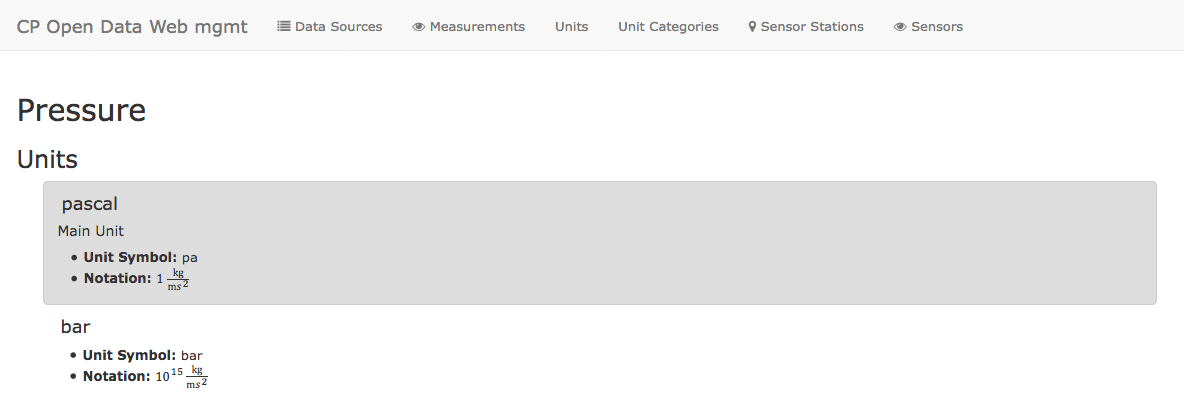
\includegraphics[width=1.00\textwidth]{images/unit_frontend.png}
	\caption{Screenshot of the units of a unit category on the web management platform. You can see the main unit and have a notation on what the units express.}
	\label{fig:screen-units}
\end{figure}

\begin{verbatim}
GET /unit_categories/:id/getMainUnit
\end{verbatim}

Example request:

\begin{verbatim}
GET /unit_categories/temperature/getMainUnit

{
    "id":"temperature_celsius",
    "name":"celsius",
    "unit_category_id":"temperature",
    "unit_symbol":"°C"
}
\end{verbatim}

\begin{verbatim}
GET /unit_categories/:id/units
\end{verbatim}

Example request:

\begin{verbatim}
GET /unit_categories/temperature/units

[
   {
      "attributes":{
         "id":"temperature_celsius",
         "name":"celsius",
         "unit_symbol":"°C",
         "unit_category_id":"temperature",
         "notation":""
      }
   },
   {
      "attributes":{
         "id":"temperature_fahrenheit",
         "name":"fahrenheit",
         "unit_symbol":"°F",
         "unit_category_id":"temperature",
         "notation":""
      }
   },
   {
      "attributes":{
         "id":"temperature_kelvin",
         "name":"kelvin",
         "unit_symbol":"K",
         "unit_category_id":"temperature",
         "notation":""
      }
   },
   ...
]
\end{verbatim}

\subsection{Discussion}\label{discussion}

As mentioned before, the planning of the extent of the functionality
offered by this system, was very vague. Besides managing metadata and
providing an API for other components, further features were at least
considered to be part of this system, like for example a scheduler that
triggers the component that handles the deployment of importers.
Therefore we chose to build this system on top of an infrastructure that
can be easily extended in many directions and has nice-to-use database
adapters instead of a more lightweight system.

While initially we also wanted to model a data source with its sensors
grouped in sensor stations, this approach would bring immense overhead
for configuring data sources in our system upfront, as a user would have
to very exactly model a data source with all its sensors and sensor
stations first. For big services like e.g.~the German Weather Service
this would be an enormous amount of work. Gathering this information
would better be done by scraping the information present in
Elasticsearch and translating them to geolocated information for all
sensors/sensor-stations/datasources. In the UML Class Diagram you can
see the modeling for this approach greyed out.

The main metainformation about the data sources (besides metadata about
the source itself) that we still needed within our system (the location
of the sensor and the grouping of sensor stations is not essential for
our system to work) and had to offer to the user registering a source
were then:

\begin{itemize}
\tightlist
\item
  Information about the measurands offered by the data source
\item
  Information about the main unit used for a measurand (see section Unit
  system)
\end{itemize}

\subsubsection{Future Improvements}\label{future-improvements}

\paragraph{Caching}

There is currently no caching solution implemented since the workloads
during development phase were quite manageable. Also including a
distributed caching system in our production pipeline seemed to be too
high of an effort and would take up significant resources that would
actually not be needed during development. We wanted, therefore, to use
the limited and expensive resources we had for actual importing.

As the number of data importers grows in production, however, requests
to the relational database would increase accordingly. Whereas scaling
the database would allow us to avoid the bottleneck, adding a cache in
front of the database to serve read requests would be sufficient to
ensure performance without incurring the cost and added complexity of
scaling. An important consideration, of course, is the frequency with
which data is updated (in our case low to none), thus making it a
perfect candidate for caching. As a distributed caching system where
read requests are very fast and possible on all nodes, Redis would be a
good fit for this use case. Writing is quite expensive due to the
replication method used by Redis, but because of the infrequent updates
to our data, we are willing to accept the trade-off in exchange for very
fast reads.

\paragraph{Exchange Scheduling information}

Due to not quite being able to reach every goal of our initial plan as
to how the architecture should look like, the scheduler had to move to
the deployment component (i.e.~the deployment to the Kubernetes
cluster). While this component should be responsible for deploying data
importers, the information about the schedule should actually be
provided to the web management system by the user. This is currently not
happening. There would be several ways how to manage scheduling and/or
deliver the scheduling information from this system to the component
handling the scheduling.

\begin{itemize}
\tightlist
\item
  Having a background processing component that acts as a scheduler
  within the web management platform. This would require an API to
  trigger the deploy on the component responsible for that, which we
  were not able to achieve.
\item
  Having a microservice-like component that is only responsible for
  scheduling and triggering importers to be deployed. This would as well
  require an API on the deployment component.
\item
  Leave the scheduling within the deployment component. This would also
  require an API, but just for receiving the general schedule, not for
  offering a hook to trigger an import.
\end{itemize}

The second option seems more granular and conforms better to our general
microservice approach but would also require the most configuration and
deployment effort. Including a scheduler in the web management platform
would somehow violate this approach but still make sense, as this
component could easily be integrated within Ruby on Rails and would be a
standalone component within it.

\section{Data Source Metadata Management System}\label{sec:metadata}

\textbf{Authoriship: } Written by Paul Wille\\
\emph{Proofread \& edited by Andres} \\

\vspace*{4mm}

In this chapter we will discuss the component responsible for managing
metadata about the data sources which are imported to the system. We
will cover what it is and does, some thoughts around why we decided to
include such a component, and how it was realized and implemented.

\subsection{Requirements}\label{requirements}

The main purpose of the component is to:

\begin{itemize}
\tightlist
\item
  serve as a registry of data sources in the system,
\item
  provide data source metadata to other components in the system,
\item
  provide users with information about units of measurement,
\item
  enable users who want to use the data to see the resources our system
  contains
\end{itemize}

In contrast to nearly every other component we had to implement, the
management platform did not have to meet as many criteria as a
distributed cloud system in general. The data it contains is quite
static and the number of requests that we expect is also quite low.
However, the following general cloud-specific architectural style
requirements were taken into consideration:

\begin{itemize}
\tightlist
\item
  Availability to other system components, that require the held
  information
\item
  Quick response time (for query optimization within the public search
  API)
\item
  Ability to run asynchronous background tasks (for scheduling)
\end{itemize}

\subsection{Implementation}\label{implementation}

The system was built using \emph{Ruby on Rails} with \emph{PostgreSQL}
as a database. The reasons why we chose to use Rails are:

\begin{itemize}
\tightlist
\item
  Relatively fast development of an MVC web application
\item
  Well established (over a decade), has therefore lots of resources ---
  also for all kinds of extensions
\item
  Extensive community support
\item
  Very good integrated ORM adapters that could easily be exchanged for
  ODM adapters for document databases
\item
  Offers the dynamic of Ruby as programming language
\end{itemize}

\subsection{Domain Model}\label{domain-model}

\begin{figure}
	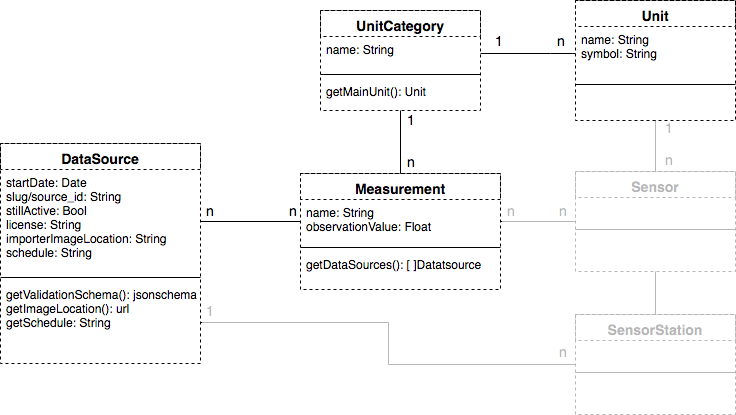
\includegraphics[width=1.00\textwidth]{images/relational_schema.png}
	\caption{UML Class Diagram of the Metadata Management System}
	\label{fig:uml-model}
\end{figure}

\subsubsection{Data Sources Registry}\label{data-sources-registry}

Before data from a given source can be imported, important information
about the source must be made available to our system. This information
consists of static metainformation and has no direct relation to actual
data being provided in the source.

We chose not to store it in the same database as the actual sensor
measurement data, but have a separate system instead. This provides
isolation between our sources and the database, preventing changes in
the choice of database or its schema from having any effect in how we
store and maintain data sources.

The metainformation that has to be provided to our system prior to
importing mainly consists of:

\begin{itemize}
\tightlist
\item
  Name of the source
\item
  Start date from which the source provides data
\item
  Whether the source is still active (i.e.~data is actively being
  provided by the source).
\item
  if not, the end date (last date for which data was provided).
\item
  Under what license the data is published
\end{itemize}

Additionally we ask the user to provide additional information, which is
useful for our system:

\begin{itemize}
\tightlist
\item
  If the data source is still active, at what schedule is new data
  published
\item
  A \emph{slug} that can be used as an id within our pipeline and in
  Elasticsearch
\item
  The measurements provided by the data source (which actual
  measurements the data source collects)
\item
  The URL location of the Docker container to be executed to import the
  data.
\end{itemize}

\begin{figure}
	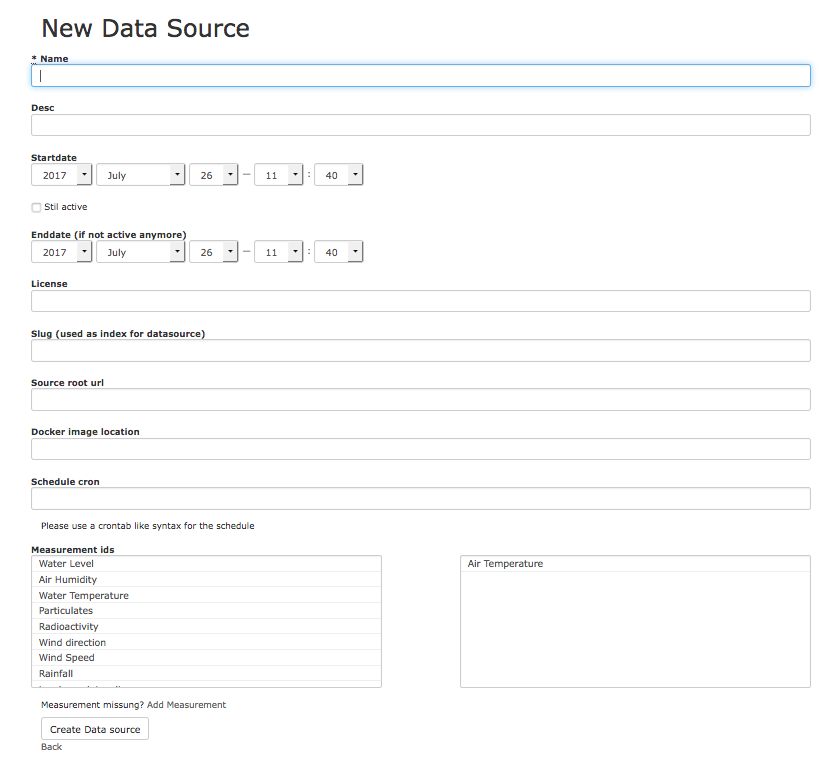
\includegraphics[width=1.00\textwidth]{images/new_datasource.png}
	\caption{Registering a data source within the Web management platform}
	\label{fig:register-source}
\end{figure}

\subsubsection{Validation Schema}\label{validation-schema}

As described in the chapter about validation and insertion into
Elasticsearch, we have a separate, distinct component that is
responsible for validating the output from data importers.

To achieve this, a schema must be provided against which to validate.
Since this schema itself is fixed, it could be hardcoded into the
validator, without the need to make another HTTP request. We decided
that this would be a bad idea for the following reasons:

\begin{itemize}
\tightlist
\item
  Sanity checks: in addition to schema-only validation, the schema
  provided by this component can validate data-source-specific values
  (such as importer IDs, etc.), which could not be validated with a
  generic validator.
\item
  Version management: schema changes over time would require changing
  the information hardcoded within the validator, and completely
  rebuilding and redeploying the validator component itself. Updating a
  record inside this component is far simpler than redeploying
  infrastructure, which is inherently more complex in an era where no
  downtime is expected.
\end{itemize}

Therefore we needed a place where said validation schema can reside. The
web management system seemed to be the right pace for that, as it
already carries metainformation about data sources and the data sources
are registered there. So it is easy to provide the relevant schema
information as well. The management system provides an API call to
supply the validation schema to the validators which looks like this:

\begin{verbatim}
GET /data_sources/:id/getValidationSchema
\end{verbatim}

The response looks like as follows (note that the const
\texttt{source\_id} would be replaced by the ID of the data source):

\begin{verbatim}
{
  "\$schema": "http://json-schema.org/schema#",
  "title": "Data Source",
  "description": "A Data Source for Open Sensor Data from the CP project \\
									at TU Berlin. ",
  "type": "object",
  "properties": {
    "source_id": {"const": "source_slug"},
    "device": {"type": "string"},
    "timestamp": { "type": "string", "format": "date-time" },
    "timestamp_data": { "type": "string", "format": "date-time" },
    "location": {
      "type": "object",
      "properties": {
        "lat": {"type": "number",
                "exclusiveMaximum": true,
                "exclusiveMinimum": true,
                "maximum": 90,
                "minimum": -90
               },
        "lon": {"type": "number",
                "exclusiveMaximum": true,
                "exclusiveMinimum": true,
                "maximum": 180,
                "minimum": -180,
               }
      },
    "required": ["lat", "lon"]
    },
    "license": {"type": "string"},
    "sensors": {
      "type": "object",
      "items": [
      {
        "type": "object",
        "properties": {
          "sensor": {"type": "string"},
          "observation_type": {"type": "string"},
          "observation_value": {"type": "number"}
        }
      }]
    }
  },
  "required": ["source_id", "timestamp","sensors", "location", "license"]
}
\end{verbatim}

\subsubsection{Provide Information to the Elasticsearch API for query
optimization}\label{provide-information-to-the-elasticsearch-api-for-query-optimization}

As described in the data model section, our model is data-source-based
and not measurand-based. For queries spanning across measurands, it will
be necessary to have further information about the relationship between
data sources and measurands.

As there were several possibilities as to where this information could
be stored and managed, and how it would be provided, the easiest place
to start with in our opinion was with the implementer of an importer,
since he or she must provide information to us when registering the data
source. The user therefore has to mark what measurements a data source
contains upfront (see Figure \ref{fig:register-source}).

In order to optimize querying, this information is provided to the API
that wraps the search interface of Elasticsearch via an API itself. The
information is stored in an indexed join table that holds the mapping
between data source and the measurands it contains. As can be seen in
the class diagram \ref{fig:uml-model} of the relational system, queries
in both directions are provided: getting all measurands for a data
source, and getting all data sources that contain a given measurand. The
corresponding routes look like this:

\begin{verbatim}
GET /data_sources/:id/measurements
\end{verbatim}

Example:

\begin{verbatim}
GET /data_sources/blume_messnetz/measurands

[
   {
      "id":1,
      "name":"Air Temperature",
      "desc":"",
      "unit_category_id":"temperature"
   },
   {
      "id":3,
      "name":"Air Humidity",
      "desc":"amount of water vapor present in the air",
      "unit_category_id":"humidity"
   }
]
\end{verbatim}

\begin{verbatim}
GET /measurements/:id/data_sources
\end{verbatim}

An example request would look like following

\begin{verbatim}
GET /measurements/1/data_sources

[
    { "id":1, "slug":"blume_messnetz", "license":"" },
    { "id":5, "slug":"german_weather_service", "license":"" }
]
\end{verbatim}

\subsubsection{Provide configuration information to the deployment
component}\label{provide-configuration-information-to-the-deployment-component}

Since the importer registration the only step in which the implementer
has to provide information to our system, it should cover all
configuration information needed to get an importer running.

\subsubsection{Units}\label{units}

With the requirements in mind, we modeled units like so:

\begin{enumerate}
\def\labelenumi{\arabic{enumi}.}
\tightlist
\item
  \textbf{Unit Categories}: Units themselves belong to a unit category.
  The unit category describes an entity for which measurements exist,
  which express their observations with one of the units of that
  category (see Figure \ref{fig:uml-model}).
\item
  Each unit has a \textbf{main unit} that we decide on. By calling the
  API or visiting the management platform a user can see, which the main
  unit is. Within our datastore we only use the main unit of a unit
  category for expressing measurements.
\item
  Units are managed by admins receptively users with permit to do so.
\item
  We therefore have a curated list of the unit categories and units
\item
  If there are units, measurements or even categories missing, each user
  can propose new ones. This proposals are also managed by the group of
  people managing the units.
\end{enumerate}

Measurements are controlled on the platform itself to allow users to
better propose new measurements, as this may happen more often. Units
and the Unit categories however are managed in a \emph{.yml} file. The
syntax we used looks like following for one entry:

\begin{verbatim}
From config/constants/units.yml:

pascal:
  id: pressure_pascal
  name: "pascal"
  unit_symbol: "pa"
  unit_category_id: pressure
  notation: "1 <centerdot>
              <mfrac>
                <mrow>
                  kg
                </mrow>
                <mrow>
                  m
                  <msup>
                          <mi>s</mi>
                          <mn>2</mn>
                </mrow>
              </mfrac>"

From config/constants/unit_categories.yml:

pressure:
  id: pressure
  name: Pressure
\end{verbatim}

The unit categories are pretty straightforward. For a unit there are
some more possibilities. Besides declaring the unit symbol, the category
it belongs to, its name you are allowed to use MathML to express what
the meaning of a unit is. This is especially helpful with units that can
be directly converted to each other (Figure \ref{fig:screen-units}).

The API of the web management system also provides calls to a) receive
the main unit of a unit category and to b) get a list of all units there
are for a unit category. Both of these information are of course aswell
accessible from the frontend of the system.

\begin{figure}[b]
	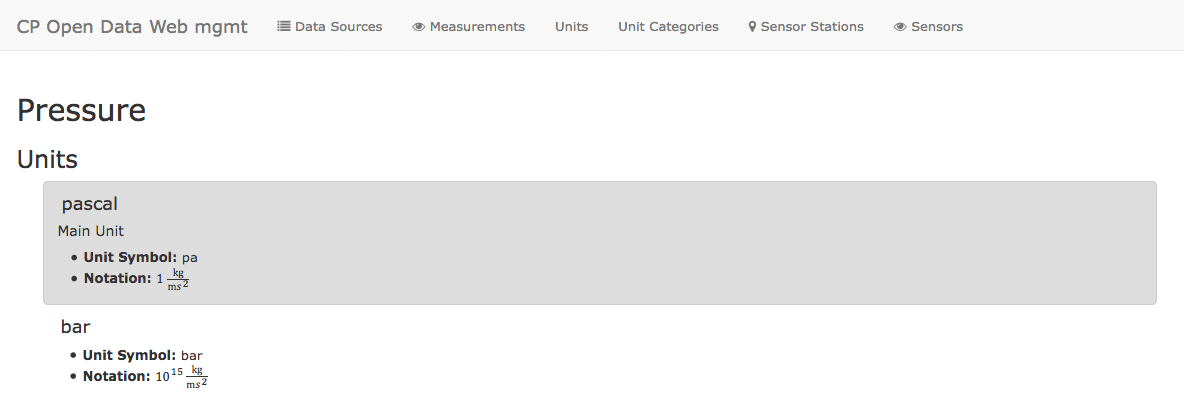
\includegraphics[width=1.00\textwidth]{images/unit_frontend.png}
	\caption{Screenshot of the units of a unit category on the web management platform. You can see the main unit and have a notation on what the units express.}
	\label{fig:screen-units}
\end{figure}

\begin{verbatim}
GET /unit_categories/:id/getMainUnit
\end{verbatim}

Example request:

\begin{verbatim}
GET /unit_categories/temperature/getMainUnit

{
    "id":"temperature_celsius",
    "name":"celsius",
    "unit_category_id":"temperature",
    "unit_symbol":"°C"
}
\end{verbatim}

\begin{verbatim}
GET /unit_categories/:id/units
\end{verbatim}

Example request:

\begin{verbatim}
GET /unit_categories/temperature/units

[
   {
      "attributes":{
         "id":"temperature_celsius",
         "name":"celsius",
         "unit_symbol":"°C",
         "unit_category_id":"temperature",
         "notation":""
      }
   },
   {
      "attributes":{
         "id":"temperature_fahrenheit",
         "name":"fahrenheit",
         "unit_symbol":"°F",
         "unit_category_id":"temperature",
         "notation":""
      }
   },
   {
      "attributes":{
         "id":"temperature_kelvin",
         "name":"kelvin",
         "unit_symbol":"K",
         "unit_category_id":"temperature",
         "notation":""
      }
   },
   ...
]
\end{verbatim}

\subsection{Discussion}\label{discussion}

As mentioned before, the planning of the extent of the functionality
offered by this system, was very vague. Besides managing metadata and
providing an API for other components, further features were at least
considered to be part of this system, like for example a scheduler that
triggers the component that handles the deployment of importers.
Therefore we chose to build this system on top of an infrastructure that
can be easily extended in many directions and has nice-to-use database
adapters instead of a more lightweight system.

While initially we also wanted to model a data source with its sensors
grouped in sensor stations, this approach would bring immense overhead
for configuring data sources in our system upfront, as a user would have
to very exactly model a data source with all its sensors and sensor
stations first. For big services like e.g.~the German Weather Service
this would be an enormous amount of work. Gathering this information
would better be done by scraping the information present in
Elasticsearch and translating them to geolocated information for all
sensors/sensor-stations/datasources. In the UML Class Diagram you can
see the modeling for this approach greyed out.

The main metainformation about the data sources (besides metadata about
the source itself) that we still needed within our system (the location
of the sensor and the grouping of sensor stations is not essential for
our system to work) and had to offer to the user registering a source
were then:

\begin{itemize}
\tightlist
\item
  Information about the measurands offered by the data source
\item
  Information about the main unit used for a measurand (see section Unit
  system)
\end{itemize}

\subsubsection{Future Improvements}\label{future-improvements}

\paragraph{Caching}

There is currently no caching solution implemented since the workloads
during development phase were quite manageable. Also including a
distributed caching system in our production pipeline seemed to be too
high of an effort and would take up significant resources that would
actually not be needed during development. We wanted, therefore, to use
the limited and expensive resources we had for actual importing.

As the number of data importers grows in production, however, requests
to the relational database would increase accordingly. Whereas scaling
the database would allow us to avoid the bottleneck, adding a cache in
front of the database to serve read requests would be sufficient to
ensure performance without incurring the cost and added complexity of
scaling. An important consideration, of course, is the frequency with
which data is updated (in our case low to none), thus making it a
perfect candidate for caching. As a distributed caching system where
read requests are very fast and possible on all nodes, Redis would be a
good fit for this use case. Writing is quite expensive due to the
replication method used by Redis, but because of the infrequent updates
to our data, we are willing to accept the trade-off in exchange for very
fast reads.

\paragraph{Exchange Scheduling information}

Due to not quite being able to reach every goal of our initial plan as
to how the architecture should look like, the scheduler had to move to
the deployment component (i.e.~the deployment to the Kubernetes
cluster). While this component should be responsible for deploying data
importers, the information about the schedule should actually be
provided to the web management system by the user. This is currently not
happening. There would be several ways how to manage scheduling and/or
deliver the scheduling information from this system to the component
handling the scheduling.

\begin{itemize}
\tightlist
\item
  Having a background processing component that acts as a scheduler
  within the web management platform. This would require an API to
  trigger the deploy on the component responsible for that, which we
  were not able to achieve.
\item
  Having a microservice-like component that is only responsible for
  scheduling and triggering importers to be deployed. This would as well
  require an API on the deployment component.
\item
  Leave the scheduling within the deployment component. This would also
  require an API, but just for receiving the general schedule, not for
  offering a hook to trigger an import.
\end{itemize}

The second option seems more granular and conforms better to our general
microservice approach but would also require the most configuration and
deployment effort. Including a scheduler in the web management platform
would somehow violate this approach but still make sense, as this
component could easily be integrated within Ruby on Rails and would be a
standalone component within it.

\section{Data Source Metadata Management System}\label{sec:metadata}

\textbf{Authoriship: } Written by Paul Wille\\
\emph{Proofread \& edited by Andres} \\

\vspace*{4mm}

In this chapter we will discuss the component responsible for managing
metadata about the data sources which are imported to the system. We
will cover what it is and does, some thoughts around why we decided to
include such a component, and how it was realized and implemented.

\subsection{Requirements}\label{requirements}

The main purpose of the component is to:

\begin{itemize}
\tightlist
\item
  serve as a registry of data sources in the system,
\item
  provide data source metadata to other components in the system,
\item
  provide users with information about units of measurement,
\item
  enable users who want to use the data to see the resources our system
  contains
\end{itemize}

In contrast to nearly every other component we had to implement, the
management platform did not have to meet as many criteria as a
distributed cloud system in general. The data it contains is quite
static and the number of requests that we expect is also quite low.
However, the following general cloud-specific architectural style
requirements were taken into consideration:

\begin{itemize}
\tightlist
\item
  Availability to other system components, that require the held
  information
\item
  Quick response time (for query optimization within the public search
  API)
\item
  Ability to run asynchronous background tasks (for scheduling)
\end{itemize}

\subsection{Implementation}\label{implementation}

The system was built using \emph{Ruby on Rails} with \emph{PostgreSQL}
as a database. The reasons why we chose to use Rails are:

\begin{itemize}
\tightlist
\item
  Relatively fast development of an MVC web application
\item
  Well established (over a decade), has therefore lots of resources ---
  also for all kinds of extensions
\item
  Extensive community support
\item
  Very good integrated ORM adapters that could easily be exchanged for
  ODM adapters for document databases
\item
  Offers the dynamic of Ruby as programming language
\end{itemize}

\subsection{Domain Model}\label{domain-model}

\begin{figure}
	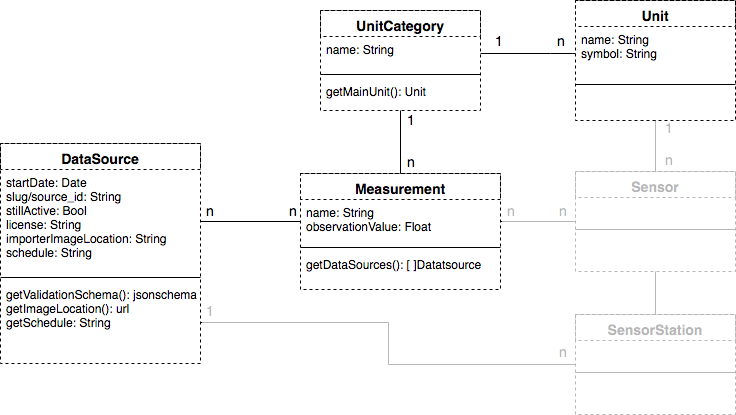
\includegraphics[width=1.00\textwidth]{images/relational_schema.png}
	\caption{UML Class Diagram of the Metadata Management System}
	\label{fig:uml-model}
\end{figure}

\subsubsection{Data Sources Registry}\label{data-sources-registry}

Before data from a given source can be imported, important information
about the source must be made available to our system. This information
consists of static metainformation and has no direct relation to actual
data being provided in the source.

We chose not to store it in the same database as the actual sensor
measurement data, but have a separate system instead. This provides
isolation between our sources and the database, preventing changes in
the choice of database or its schema from having any effect in how we
store and maintain data sources.

The metainformation that has to be provided to our system prior to
importing mainly consists of:

\begin{itemize}
\tightlist
\item
  Name of the source
\item
  Start date from which the source provides data
\item
  Whether the source is still active (i.e.~data is actively being
  provided by the source).
\item
  if not, the end date (last date for which data was provided).
\item
  Under what license the data is published
\end{itemize}

Additionally we ask the user to provide additional information, which is
useful for our system:

\begin{itemize}
\tightlist
\item
  If the data source is still active, at what schedule is new data
  published
\item
  A \emph{slug} that can be used as an id within our pipeline and in
  Elasticsearch
\item
  The measurements provided by the data source (which actual
  measurements the data source collects)
\item
  The URL location of the Docker container to be executed to import the
  data.
\end{itemize}

\begin{figure}
	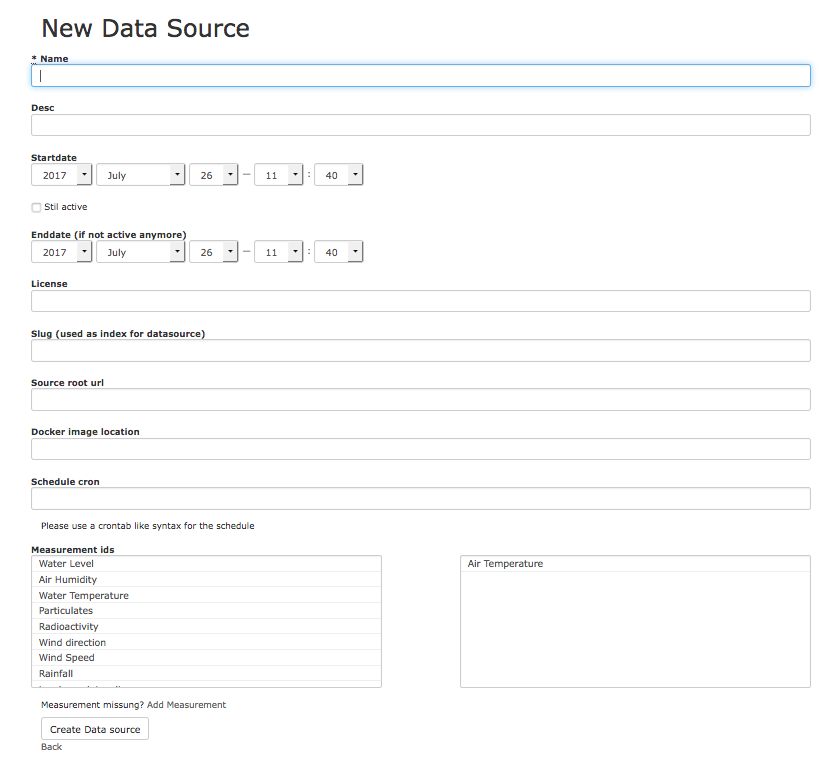
\includegraphics[width=1.00\textwidth]{images/new_datasource.png}
	\caption{Registering a data source within the Web management platform}
	\label{fig:register-source}
\end{figure}

\subsubsection{Validation Schema}\label{validation-schema}

As described in the chapter about validation and insertion into
Elasticsearch, we have a separate, distinct component that is
responsible for validating the output from data importers.

To achieve this, a schema must be provided against which to validate.
Since this schema itself is fixed, it could be hardcoded into the
validator, without the need to make another HTTP request. We decided
that this would be a bad idea for the following reasons:

\begin{itemize}
\tightlist
\item
  Sanity checks: in addition to schema-only validation, the schema
  provided by this component can validate data-source-specific values
  (such as importer IDs, etc.), which could not be validated with a
  generic validator.
\item
  Version management: schema changes over time would require changing
  the information hardcoded within the validator, and completely
  rebuilding and redeploying the validator component itself. Updating a
  record inside this component is far simpler than redeploying
  infrastructure, which is inherently more complex in an era where no
  downtime is expected.
\end{itemize}

Therefore we needed a place where said validation schema can reside. The
web management system seemed to be the right pace for that, as it
already carries metainformation about data sources and the data sources
are registered there. So it is easy to provide the relevant schema
information as well. The management system provides an API call to
supply the validation schema to the validators which looks like this:

\begin{verbatim}
GET /data_sources/:id/getValidationSchema
\end{verbatim}

The response looks like as follows (note that the const
\texttt{source\_id} would be replaced by the ID of the data source):

\begin{verbatim}
{
  "\$schema": "http://json-schema.org/schema#",
  "title": "Data Source",
  "description": "A Data Source for Open Sensor Data from the CP project \\
									at TU Berlin. ",
  "type": "object",
  "properties": {
    "source_id": {"const": "source_slug"},
    "device": {"type": "string"},
    "timestamp": { "type": "string", "format": "date-time" },
    "timestamp_data": { "type": "string", "format": "date-time" },
    "location": {
      "type": "object",
      "properties": {
        "lat": {"type": "number",
                "exclusiveMaximum": true,
                "exclusiveMinimum": true,
                "maximum": 90,
                "minimum": -90
               },
        "lon": {"type": "number",
                "exclusiveMaximum": true,
                "exclusiveMinimum": true,
                "maximum": 180,
                "minimum": -180,
               }
      },
    "required": ["lat", "lon"]
    },
    "license": {"type": "string"},
    "sensors": {
      "type": "object",
      "items": [
      {
        "type": "object",
        "properties": {
          "sensor": {"type": "string"},
          "observation_type": {"type": "string"},
          "observation_value": {"type": "number"}
        }
      }]
    }
  },
  "required": ["source_id", "timestamp","sensors", "location", "license"]
}
\end{verbatim}

\subsubsection{Provide Information to the Elasticsearch API for query
optimization}\label{provide-information-to-the-elasticsearch-api-for-query-optimization}

As described in the data model section, our model is data-source-based
and not measurand-based. For queries spanning across measurands, it will
be necessary to have further information about the relationship between
data sources and measurands.

As there were several possibilities as to where this information could
be stored and managed, and how it would be provided, the easiest place
to start with in our opinion was with the implementer of an importer,
since he or she must provide information to us when registering the data
source. The user therefore has to mark what measurements a data source
contains upfront (see Figure \ref{fig:register-source}).

In order to optimize querying, this information is provided to the API
that wraps the search interface of Elasticsearch via an API itself. The
information is stored in an indexed join table that holds the mapping
between data source and the measurands it contains. As can be seen in
the class diagram \ref{fig:uml-model} of the relational system, queries
in both directions are provided: getting all measurands for a data
source, and getting all data sources that contain a given measurand. The
corresponding routes look like this:

\begin{verbatim}
GET /data_sources/:id/measurements
\end{verbatim}

Example:

\begin{verbatim}
GET /data_sources/blume_messnetz/measurands

[
   {
      "id":1,
      "name":"Air Temperature",
      "desc":"",
      "unit_category_id":"temperature"
   },
   {
      "id":3,
      "name":"Air Humidity",
      "desc":"amount of water vapor present in the air",
      "unit_category_id":"humidity"
   }
]
\end{verbatim}

\begin{verbatim}
GET /measurements/:id/data_sources
\end{verbatim}

An example request would look like following

\begin{verbatim}
GET /measurements/1/data_sources

[
    { "id":1, "slug":"blume_messnetz", "license":"" },
    { "id":5, "slug":"german_weather_service", "license":"" }
]
\end{verbatim}

\subsubsection{Provide configuration information to the deployment
component}\label{provide-configuration-information-to-the-deployment-component}

Since the importer registration the only step in which the implementer
has to provide information to our system, it should cover all
configuration information needed to get an importer running.

\subsubsection{Units}\label{units}

With the requirements in mind, we modeled units like so:

\begin{enumerate}
\def\labelenumi{\arabic{enumi}.}
\tightlist
\item
  \textbf{Unit Categories}: Units themselves belong to a unit category.
  The unit category describes an entity for which measurements exist,
  which express their observations with one of the units of that
  category (see Figure \ref{fig:uml-model}).
\item
  Each unit has a \textbf{main unit} that we decide on. By calling the
  API or visiting the management platform a user can see, which the main
  unit is. Within our datastore we only use the main unit of a unit
  category for expressing measurements.
\item
  Units are managed by admins receptively users with permit to do so.
\item
  We therefore have a curated list of the unit categories and units
\item
  If there are units, measurements or even categories missing, each user
  can propose new ones. This proposals are also managed by the group of
  people managing the units.
\end{enumerate}

Measurements are controlled on the platform itself to allow users to
better propose new measurements, as this may happen more often. Units
and the Unit categories however are managed in a \emph{.yml} file. The
syntax we used looks like following for one entry:

\begin{verbatim}
From config/constants/units.yml:

pascal:
  id: pressure_pascal
  name: "pascal"
  unit_symbol: "pa"
  unit_category_id: pressure
  notation: "1 <centerdot>
              <mfrac>
                <mrow>
                  kg
                </mrow>
                <mrow>
                  m
                  <msup>
                          <mi>s</mi>
                          <mn>2</mn>
                </mrow>
              </mfrac>"

From config/constants/unit_categories.yml:

pressure:
  id: pressure
  name: Pressure
\end{verbatim}

The unit categories are pretty straightforward. For a unit there are
some more possibilities. Besides declaring the unit symbol, the category
it belongs to, its name you are allowed to use MathML to express what
the meaning of a unit is. This is especially helpful with units that can
be directly converted to each other (Figure \ref{fig:screen-units}).

The API of the web management system also provides calls to a) receive
the main unit of a unit category and to b) get a list of all units there
are for a unit category. Both of these information are of course aswell
accessible from the frontend of the system.

\begin{figure}[b]
	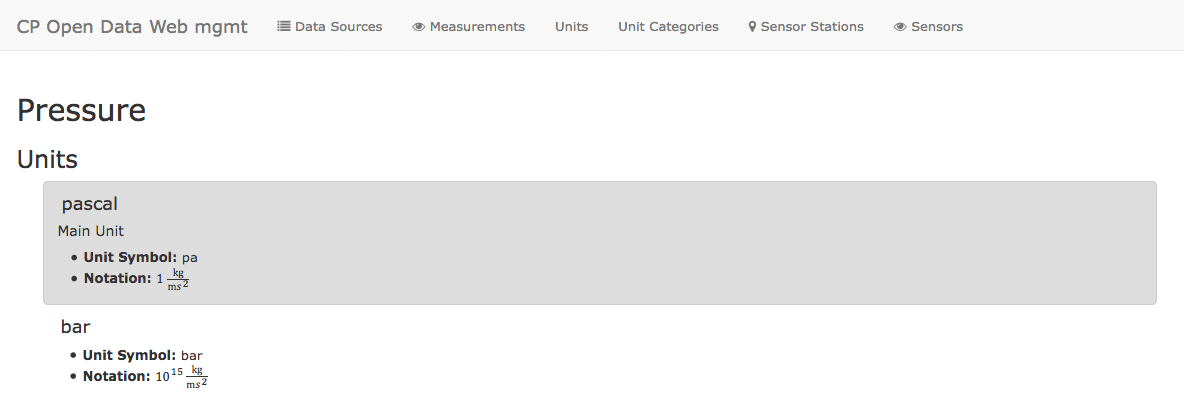
\includegraphics[width=1.00\textwidth]{images/unit_frontend.png}
	\caption{Screenshot of the units of a unit category on the web management platform. You can see the main unit and have a notation on what the units express.}
	\label{fig:screen-units}
\end{figure}

\begin{verbatim}
GET /unit_categories/:id/getMainUnit
\end{verbatim}

Example request:

\begin{verbatim}
GET /unit_categories/temperature/getMainUnit

{
    "id":"temperature_celsius",
    "name":"celsius",
    "unit_category_id":"temperature",
    "unit_symbol":"°C"
}
\end{verbatim}

\begin{verbatim}
GET /unit_categories/:id/units
\end{verbatim}

Example request:

\begin{verbatim}
GET /unit_categories/temperature/units

[
   {
      "attributes":{
         "id":"temperature_celsius",
         "name":"celsius",
         "unit_symbol":"°C",
         "unit_category_id":"temperature",
         "notation":""
      }
   },
   {
      "attributes":{
         "id":"temperature_fahrenheit",
         "name":"fahrenheit",
         "unit_symbol":"°F",
         "unit_category_id":"temperature",
         "notation":""
      }
   },
   {
      "attributes":{
         "id":"temperature_kelvin",
         "name":"kelvin",
         "unit_symbol":"K",
         "unit_category_id":"temperature",
         "notation":""
      }
   },
   ...
]
\end{verbatim}

\subsection{Discussion}\label{discussion}

As mentioned before, the planning of the extent of the functionality
offered by this system, was very vague. Besides managing metadata and
providing an API for other components, further features were at least
considered to be part of this system, like for example a scheduler that
triggers the component that handles the deployment of importers.
Therefore we chose to build this system on top of an infrastructure that
can be easily extended in many directions and has nice-to-use database
adapters instead of a more lightweight system.

While initially we also wanted to model a data source with its sensors
grouped in sensor stations, this approach would bring immense overhead
for configuring data sources in our system upfront, as a user would have
to very exactly model a data source with all its sensors and sensor
stations first. For big services like e.g.~the German Weather Service
this would be an enormous amount of work. Gathering this information
would better be done by scraping the information present in
Elasticsearch and translating them to geolocated information for all
sensors/sensor-stations/datasources. In the UML Class Diagram you can
see the modeling for this approach greyed out.

The main metainformation about the data sources (besides metadata about
the source itself) that we still needed within our system (the location
of the sensor and the grouping of sensor stations is not essential for
our system to work) and had to offer to the user registering a source
were then:

\begin{itemize}
\tightlist
\item
  Information about the measurands offered by the data source
\item
  Information about the main unit used for a measurand (see section Unit
  system)
\end{itemize}

\subsubsection{Future Improvements}\label{future-improvements}

\paragraph{Caching}

There is currently no caching solution implemented since the workloads
during development phase were quite manageable. Also including a
distributed caching system in our production pipeline seemed to be too
high of an effort and would take up significant resources that would
actually not be needed during development. We wanted, therefore, to use
the limited and expensive resources we had for actual importing.

As the number of data importers grows in production, however, requests
to the relational database would increase accordingly. Whereas scaling
the database would allow us to avoid the bottleneck, adding a cache in
front of the database to serve read requests would be sufficient to
ensure performance without incurring the cost and added complexity of
scaling. An important consideration, of course, is the frequency with
which data is updated (in our case low to none), thus making it a
perfect candidate for caching. As a distributed caching system where
read requests are very fast and possible on all nodes, Redis would be a
good fit for this use case. Writing is quite expensive due to the
replication method used by Redis, but because of the infrequent updates
to our data, we are willing to accept the trade-off in exchange for very
fast reads.

\paragraph{Exchange Scheduling information}

Due to not quite being able to reach every goal of our initial plan as
to how the architecture should look like, the scheduler had to move to
the deployment component (i.e.~the deployment to the Kubernetes
cluster). While this component should be responsible for deploying data
importers, the information about the schedule should actually be
provided to the web management system by the user. This is currently not
happening. There would be several ways how to manage scheduling and/or
deliver the scheduling information from this system to the component
handling the scheduling.

\begin{itemize}
\tightlist
\item
  Having a background processing component that acts as a scheduler
  within the web management platform. This would require an API to
  trigger the deploy on the component responsible for that, which we
  were not able to achieve.
\item
  Having a microservice-like component that is only responsible for
  scheduling and triggering importers to be deployed. This would as well
  require an API on the deployment component.
\item
  Leave the scheduling within the deployment component. This would also
  require an API, but just for receiving the general schedule, not for
  offering a hook to trigger an import.
\end{itemize}

The second option seems more granular and conforms better to our general
microservice approach but would also require the most configuration and
deployment effort. Including a scheduler in the web management platform
would somehow violate this approach but still make sense, as this
component could easily be integrated within Ruby on Rails and would be a
standalone component within it.

\section{Data Source Metadata Management System}\label{sec:metadata}

\textbf{Authoriship: } Written by Paul Wille\\
\emph{Proofread \& edited by Andres} \\

\vspace*{4mm}

In this chapter we will discuss the component responsible for managing
metadata about the data sources which are imported to the system. We
will cover what it is and does, some thoughts around why we decided to
include such a component, and how it was realized and implemented.

\subsection{Requirements}\label{requirements}

The main purpose of the component is to:

\begin{itemize}
\tightlist
\item
  serve as a registry of data sources in the system,
\item
  provide data source metadata to other components in the system,
\item
  provide users with information about units of measurement,
\item
  enable users who want to use the data to see the resources our system
  contains
\end{itemize}

In contrast to nearly every other component we had to implement, the
management platform did not have to meet as many criteria as a
distributed cloud system in general. The data it contains is quite
static and the number of requests that we expect is also quite low.
However, the following general cloud-specific architectural style
requirements were taken into consideration:

\begin{itemize}
\tightlist
\item
  Availability to other system components, that require the held
  information
\item
  Quick response time (for query optimization within the public search
  API)
\item
  Ability to run asynchronous background tasks (for scheduling)
\end{itemize}

\subsection{Implementation}\label{implementation}

The system was built using \emph{Ruby on Rails} with \emph{PostgreSQL}
as a database. The reasons why we chose to use Rails are:

\begin{itemize}
\tightlist
\item
  Relatively fast development of an MVC web application
\item
  Well established (over a decade), has therefore lots of resources ---
  also for all kinds of extensions
\item
  Extensive community support
\item
  Very good integrated ORM adapters that could easily be exchanged for
  ODM adapters for document databases
\item
  Offers the dynamic of Ruby as programming language
\end{itemize}

\subsection{Domain Model}\label{domain-model}

\begin{figure}
	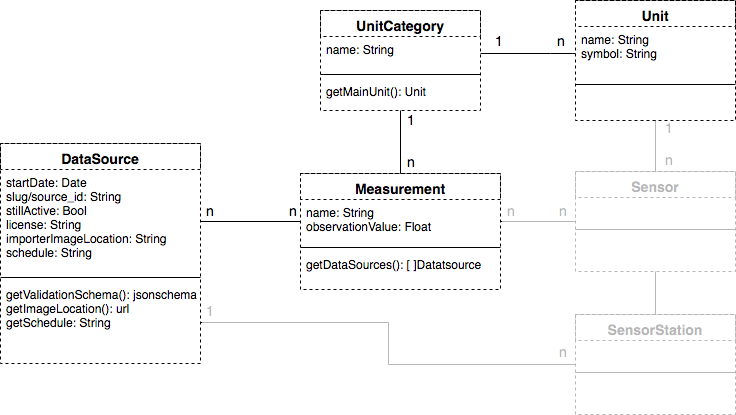
\includegraphics[width=1.00\textwidth]{images/relational_schema.png}
	\caption{UML Class Diagram of the Metadata Management System}
	\label{fig:uml-model}
\end{figure}

\subsubsection{Data Sources Registry}\label{data-sources-registry}

Before data from a given source can be imported, important information
about the source must be made available to our system. This information
consists of static metainformation and has no direct relation to actual
data being provided in the source.

We chose not to store it in the same database as the actual sensor
measurement data, but have a separate system instead. This provides
isolation between our sources and the database, preventing changes in
the choice of database or its schema from having any effect in how we
store and maintain data sources.

The metainformation that has to be provided to our system prior to
importing mainly consists of:

\begin{itemize}
\tightlist
\item
  Name of the source
\item
  Start date from which the source provides data
\item
  Whether the source is still active (i.e.~data is actively being
  provided by the source).
\item
  if not, the end date (last date for which data was provided).
\item
  Under what license the data is published
\end{itemize}

Additionally we ask the user to provide additional information, which is
useful for our system:

\begin{itemize}
\tightlist
\item
  If the data source is still active, at what schedule is new data
  published
\item
  A \emph{slug} that can be used as an id within our pipeline and in
  Elasticsearch
\item
  The measurements provided by the data source (which actual
  measurements the data source collects)
\item
  The URL location of the Docker container to be executed to import the
  data.
\end{itemize}

\begin{figure}
	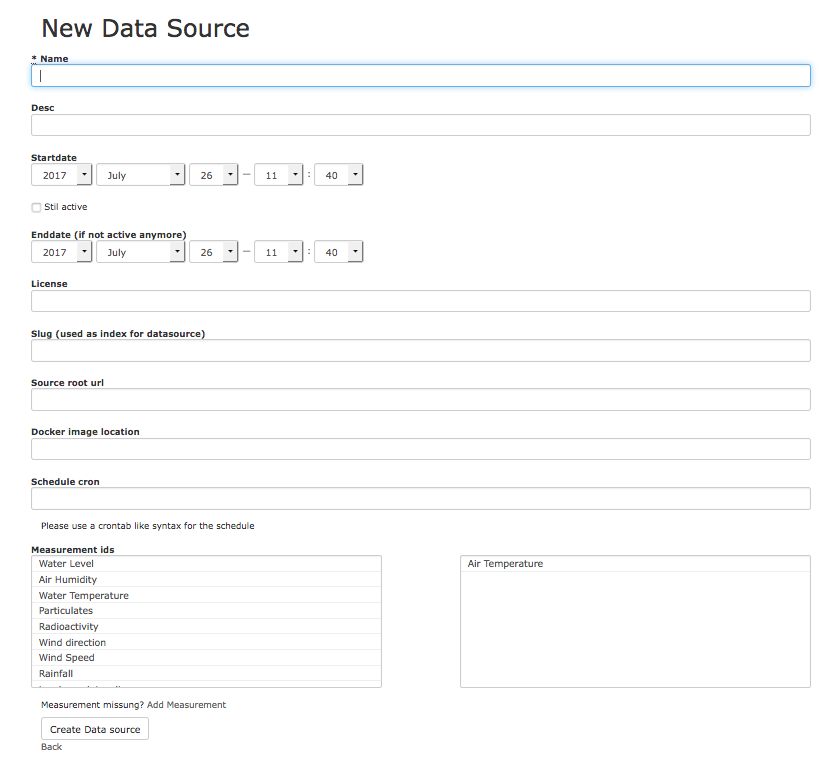
\includegraphics[width=1.00\textwidth]{images/new_datasource.png}
	\caption{Registering a data source within the Web management platform}
	\label{fig:register-source}
\end{figure}

\subsubsection{Validation Schema}\label{validation-schema}

As described in the chapter about validation and insertion into
Elasticsearch, we have a separate, distinct component that is
responsible for validating the output from data importers.

To achieve this, a schema must be provided against which to validate.
Since this schema itself is fixed, it could be hardcoded into the
validator, without the need to make another HTTP request. We decided
that this would be a bad idea for the following reasons:

\begin{itemize}
\tightlist
\item
  Sanity checks: in addition to schema-only validation, the schema
  provided by this component can validate data-source-specific values
  (such as importer IDs, etc.), which could not be validated with a
  generic validator.
\item
  Version management: schema changes over time would require changing
  the information hardcoded within the validator, and completely
  rebuilding and redeploying the validator component itself. Updating a
  record inside this component is far simpler than redeploying
  infrastructure, which is inherently more complex in an era where no
  downtime is expected.
\end{itemize}

Therefore we needed a place where said validation schema can reside. The
web management system seemed to be the right pace for that, as it
already carries metainformation about data sources and the data sources
are registered there. So it is easy to provide the relevant schema
information as well. The management system provides an API call to
supply the validation schema to the validators which looks like this:

\begin{verbatim}
GET /data_sources/:id/getValidationSchema
\end{verbatim}

The response looks like as follows (note that the const
\texttt{source\_id} would be replaced by the ID of the data source):

\begin{verbatim}
{
  "\$schema": "http://json-schema.org/schema#",
  "title": "Data Source",
  "description": "A Data Source for Open Sensor Data from the CP project \\
									at TU Berlin. ",
  "type": "object",
  "properties": {
    "source_id": {"const": "source_slug"},
    "device": {"type": "string"},
    "timestamp": { "type": "string", "format": "date-time" },
    "timestamp_data": { "type": "string", "format": "date-time" },
    "location": {
      "type": "object",
      "properties": {
        "lat": {"type": "number",
                "exclusiveMaximum": true,
                "exclusiveMinimum": true,
                "maximum": 90,
                "minimum": -90
               },
        "lon": {"type": "number",
                "exclusiveMaximum": true,
                "exclusiveMinimum": true,
                "maximum": 180,
                "minimum": -180,
               }
      },
    "required": ["lat", "lon"]
    },
    "license": {"type": "string"},
    "sensors": {
      "type": "object",
      "items": [
      {
        "type": "object",
        "properties": {
          "sensor": {"type": "string"},
          "observation_type": {"type": "string"},
          "observation_value": {"type": "number"}
        }
      }]
    }
  },
  "required": ["source_id", "timestamp","sensors", "location", "license"]
}
\end{verbatim}

\subsubsection{Provide Information to the Elasticsearch API for query
optimization}\label{provide-information-to-the-elasticsearch-api-for-query-optimization}

As described in the data model section, our model is data-source-based
and not measurand-based. For queries spanning across measurands, it will
be necessary to have further information about the relationship between
data sources and measurands.

As there were several possibilities as to where this information could
be stored and managed, and how it would be provided, the easiest place
to start with in our opinion was with the implementer of an importer,
since he or she must provide information to us when registering the data
source. The user therefore has to mark what measurements a data source
contains upfront (see Figure \ref{fig:register-source}).

In order to optimize querying, this information is provided to the API
that wraps the search interface of Elasticsearch via an API itself. The
information is stored in an indexed join table that holds the mapping
between data source and the measurands it contains. As can be seen in
the class diagram \ref{fig:uml-model} of the relational system, queries
in both directions are provided: getting all measurands for a data
source, and getting all data sources that contain a given measurand. The
corresponding routes look like this:

\begin{verbatim}
GET /data_sources/:id/measurements
\end{verbatim}

Example:

\begin{verbatim}
GET /data_sources/blume_messnetz/measurands

[
   {
      "id":1,
      "name":"Air Temperature",
      "desc":"",
      "unit_category_id":"temperature"
   },
   {
      "id":3,
      "name":"Air Humidity",
      "desc":"amount of water vapor present in the air",
      "unit_category_id":"humidity"
   }
]
\end{verbatim}

\begin{verbatim}
GET /measurements/:id/data_sources
\end{verbatim}

An example request would look like following

\begin{verbatim}
GET /measurements/1/data_sources

[
    { "id":1, "slug":"blume_messnetz", "license":"" },
    { "id":5, "slug":"german_weather_service", "license":"" }
]
\end{verbatim}

\subsubsection{Provide configuration information to the deployment
component}\label{provide-configuration-information-to-the-deployment-component}

Since the importer registration the only step in which the implementer
has to provide information to our system, it should cover all
configuration information needed to get an importer running.

\subsubsection{Units}\label{units}

With the requirements in mind, we modeled units like so:

\begin{enumerate}
\def\labelenumi{\arabic{enumi}.}
\tightlist
\item
  \textbf{Unit Categories}: Units themselves belong to a unit category.
  The unit category describes an entity for which measurements exist,
  which express their observations with one of the units of that
  category (see Figure \ref{fig:uml-model}).
\item
  Each unit has a \textbf{main unit} that we decide on. By calling the
  API or visiting the management platform a user can see, which the main
  unit is. Within our datastore we only use the main unit of a unit
  category for expressing measurements.
\item
  Units are managed by admins receptively users with permit to do so.
\item
  We therefore have a curated list of the unit categories and units
\item
  If there are units, measurements or even categories missing, each user
  can propose new ones. This proposals are also managed by the group of
  people managing the units.
\end{enumerate}

Measurements are controlled on the platform itself to allow users to
better propose new measurements, as this may happen more often. Units
and the Unit categories however are managed in a \emph{.yml} file. The
syntax we used looks like following for one entry:

\begin{verbatim}
From config/constants/units.yml:

pascal:
  id: pressure_pascal
  name: "pascal"
  unit_symbol: "pa"
  unit_category_id: pressure
  notation: "1 <centerdot>
              <mfrac>
                <mrow>
                  kg
                </mrow>
                <mrow>
                  m
                  <msup>
                          <mi>s</mi>
                          <mn>2</mn>
                </mrow>
              </mfrac>"

From config/constants/unit_categories.yml:

pressure:
  id: pressure
  name: Pressure
\end{verbatim}

The unit categories are pretty straightforward. For a unit there are
some more possibilities. Besides declaring the unit symbol, the category
it belongs to, its name you are allowed to use MathML to express what
the meaning of a unit is. This is especially helpful with units that can
be directly converted to each other (Figure \ref{fig:screen-units}).

The API of the web management system also provides calls to a) receive
the main unit of a unit category and to b) get a list of all units there
are for a unit category. Both of these information are of course aswell
accessible from the frontend of the system.

\begin{figure}[b]
	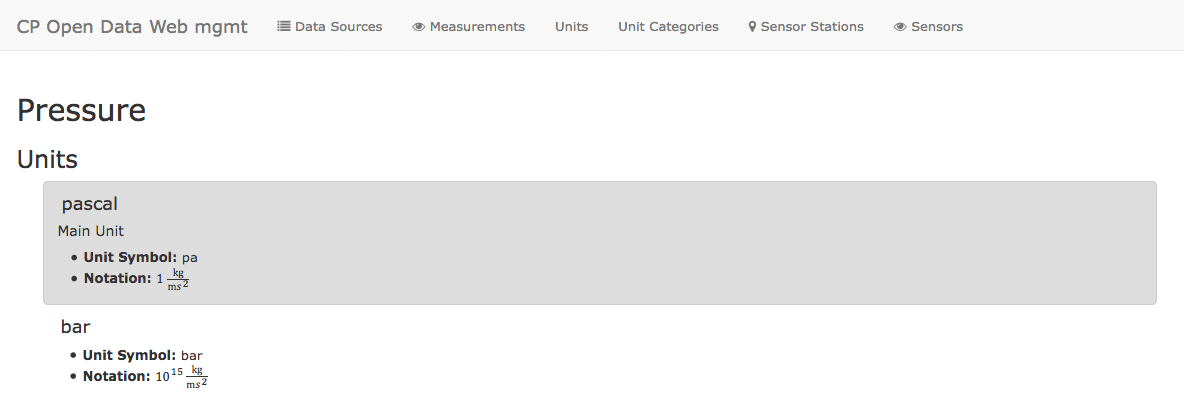
\includegraphics[width=1.00\textwidth]{images/unit_frontend.png}
	\caption{Screenshot of the units of a unit category on the web management platform. You can see the main unit and have a notation on what the units express.}
	\label{fig:screen-units}
\end{figure}

\begin{verbatim}
GET /unit_categories/:id/getMainUnit
\end{verbatim}

Example request:

\begin{verbatim}
GET /unit_categories/temperature/getMainUnit

{
    "id":"temperature_celsius",
    "name":"celsius",
    "unit_category_id":"temperature",
    "unit_symbol":"°C"
}
\end{verbatim}

\begin{verbatim}
GET /unit_categories/:id/units
\end{verbatim}

Example request:

\begin{verbatim}
GET /unit_categories/temperature/units

[
   {
      "attributes":{
         "id":"temperature_celsius",
         "name":"celsius",
         "unit_symbol":"°C",
         "unit_category_id":"temperature",
         "notation":""
      }
   },
   {
      "attributes":{
         "id":"temperature_fahrenheit",
         "name":"fahrenheit",
         "unit_symbol":"°F",
         "unit_category_id":"temperature",
         "notation":""
      }
   },
   {
      "attributes":{
         "id":"temperature_kelvin",
         "name":"kelvin",
         "unit_symbol":"K",
         "unit_category_id":"temperature",
         "notation":""
      }
   },
   ...
]
\end{verbatim}

\subsection{Discussion}\label{discussion}

As mentioned before, the planning of the extent of the functionality
offered by this system, was very vague. Besides managing metadata and
providing an API for other components, further features were at least
considered to be part of this system, like for example a scheduler that
triggers the component that handles the deployment of importers.
Therefore we chose to build this system on top of an infrastructure that
can be easily extended in many directions and has nice-to-use database
adapters instead of a more lightweight system.

While initially we also wanted to model a data source with its sensors
grouped in sensor stations, this approach would bring immense overhead
for configuring data sources in our system upfront, as a user would have
to very exactly model a data source with all its sensors and sensor
stations first. For big services like e.g.~the German Weather Service
this would be an enormous amount of work. Gathering this information
would better be done by scraping the information present in
Elasticsearch and translating them to geolocated information for all
sensors/sensor-stations/datasources. In the UML Class Diagram you can
see the modeling for this approach greyed out.

The main metainformation about the data sources (besides metadata about
the source itself) that we still needed within our system (the location
of the sensor and the grouping of sensor stations is not essential for
our system to work) and had to offer to the user registering a source
were then:

\begin{itemize}
\tightlist
\item
  Information about the measurands offered by the data source
\item
  Information about the main unit used for a measurand (see section Unit
  system)
\end{itemize}

\subsubsection{Future Improvements}\label{future-improvements}

\paragraph{Caching}

There is currently no caching solution implemented since the workloads
during development phase were quite manageable. Also including a
distributed caching system in our production pipeline seemed to be too
high of an effort and would take up significant resources that would
actually not be needed during development. We wanted, therefore, to use
the limited and expensive resources we had for actual importing.

As the number of data importers grows in production, however, requests
to the relational database would increase accordingly. Whereas scaling
the database would allow us to avoid the bottleneck, adding a cache in
front of the database to serve read requests would be sufficient to
ensure performance without incurring the cost and added complexity of
scaling. An important consideration, of course, is the frequency with
which data is updated (in our case low to none), thus making it a
perfect candidate for caching. As a distributed caching system where
read requests are very fast and possible on all nodes, Redis would be a
good fit for this use case. Writing is quite expensive due to the
replication method used by Redis, but because of the infrequent updates
to our data, we are willing to accept the trade-off in exchange for very
fast reads.

\paragraph{Exchange Scheduling information}

Due to not quite being able to reach every goal of our initial plan as
to how the architecture should look like, the scheduler had to move to
the deployment component (i.e.~the deployment to the Kubernetes
cluster). While this component should be responsible for deploying data
importers, the information about the schedule should actually be
provided to the web management system by the user. This is currently not
happening. There would be several ways how to manage scheduling and/or
deliver the scheduling information from this system to the component
handling the scheduling.

\begin{itemize}
\tightlist
\item
  Having a background processing component that acts as a scheduler
  within the web management platform. This would require an API to
  trigger the deploy on the component responsible for that, which we
  were not able to achieve.
\item
  Having a microservice-like component that is only responsible for
  scheduling and triggering importers to be deployed. This would as well
  require an API on the deployment component.
\item
  Leave the scheduling within the deployment component. This would also
  require an API, but just for receiving the general schedule, not for
  offering a hook to trigger an import.
\end{itemize}

The second option seems more granular and conforms better to our general
microservice approach but would also require the most configuration and
deployment effort. Including a scheduler in the web management platform
would somehow violate this approach but still make sense, as this
component could easily be integrated within Ruby on Rails and would be a
standalone component within it.

\section{Data Source Metadata Management System}\label{sec:metadata}

\textbf{Authoriship: } Written by Paul Wille\\
\emph{Proofread \& edited by Andres} \\

\vspace*{4mm}

In this chapter we will discuss the component responsible for managing
metadata about the data sources which are imported to the system. We
will cover what it is and does, some thoughts around why we decided to
include such a component, and how it was realized and implemented.

\subsection{Requirements}\label{requirements}

The main purpose of the component is to:

\begin{itemize}
\tightlist
\item
  serve as a registry of data sources in the system,
\item
  provide data source metadata to other components in the system,
\item
  provide users with information about units of measurement,
\item
  enable users who want to use the data to see the resources our system
  contains
\end{itemize}

In contrast to nearly every other component we had to implement, the
management platform did not have to meet as many criteria as a
distributed cloud system in general. The data it contains is quite
static and the number of requests that we expect is also quite low.
However, the following general cloud-specific architectural style
requirements were taken into consideration:

\begin{itemize}
\tightlist
\item
  Availability to other system components, that require the held
  information
\item
  Quick response time (for query optimization within the public search
  API)
\item
  Ability to run asynchronous background tasks (for scheduling)
\end{itemize}

\subsection{Implementation}\label{implementation}

The system was built using \emph{Ruby on Rails} with \emph{PostgreSQL}
as a database. The reasons why we chose to use Rails are:

\begin{itemize}
\tightlist
\item
  Relatively fast development of an MVC web application
\item
  Well established (over a decade), has therefore lots of resources ---
  also for all kinds of extensions
\item
  Extensive community support
\item
  Very good integrated ORM adapters that could easily be exchanged for
  ODM adapters for document databases
\item
  Offers the dynamic of Ruby as programming language
\end{itemize}

\subsection{Domain Model}\label{domain-model}

\begin{figure}
	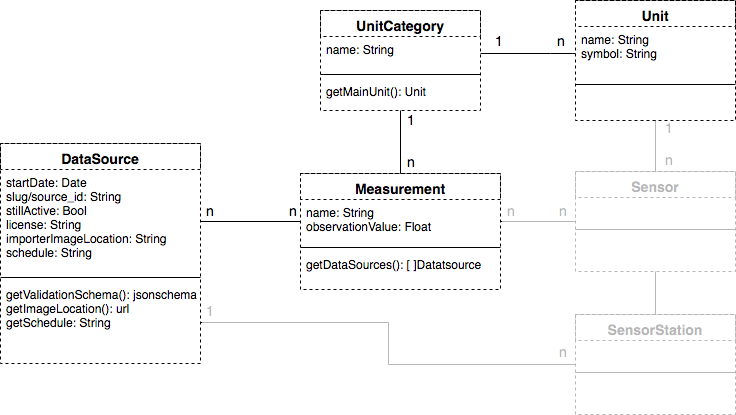
\includegraphics[width=1.00\textwidth]{images/relational_schema.png}
	\caption{UML Class Diagram of the Metadata Management System}
	\label{fig:uml-model}
\end{figure}

\subsubsection{Data Sources Registry}\label{data-sources-registry}

Before data from a given source can be imported, important information
about the source must be made available to our system. This information
consists of static metainformation and has no direct relation to actual
data being provided in the source.

We chose not to store it in the same database as the actual sensor
measurement data, but have a separate system instead. This provides
isolation between our sources and the database, preventing changes in
the choice of database or its schema from having any effect in how we
store and maintain data sources.

The metainformation that has to be provided to our system prior to
importing mainly consists of:

\begin{itemize}
\tightlist
\item
  Name of the source
\item
  Start date from which the source provides data
\item
  Whether the source is still active (i.e.~data is actively being
  provided by the source).
\item
  if not, the end date (last date for which data was provided).
\item
  Under what license the data is published
\end{itemize}

Additionally we ask the user to provide additional information, which is
useful for our system:

\begin{itemize}
\tightlist
\item
  If the data source is still active, at what schedule is new data
  published
\item
  A \emph{slug} that can be used as an id within our pipeline and in
  Elasticsearch
\item
  The measurements provided by the data source (which actual
  measurements the data source collects)
\item
  The URL location of the Docker container to be executed to import the
  data.
\end{itemize}

\begin{figure}
	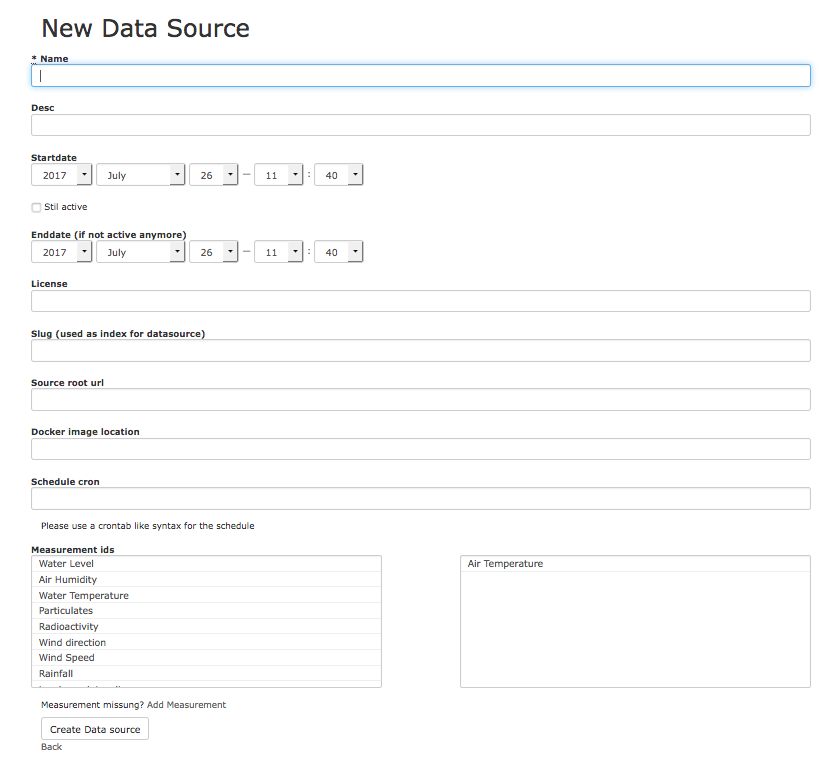
\includegraphics[width=1.00\textwidth]{images/new_datasource.png}
	\caption{Registering a data source within the Web management platform}
	\label{fig:register-source}
\end{figure}

\subsubsection{Validation Schema}\label{validation-schema}

As described in the chapter about validation and insertion into
Elasticsearch, we have a separate, distinct component that is
responsible for validating the output from data importers.

To achieve this, a schema must be provided against which to validate.
Since this schema itself is fixed, it could be hardcoded into the
validator, without the need to make another HTTP request. We decided
that this would be a bad idea for the following reasons:

\begin{itemize}
\tightlist
\item
  Sanity checks: in addition to schema-only validation, the schema
  provided by this component can validate data-source-specific values
  (such as importer IDs, etc.), which could not be validated with a
  generic validator.
\item
  Version management: schema changes over time would require changing
  the information hardcoded within the validator, and completely
  rebuilding and redeploying the validator component itself. Updating a
  record inside this component is far simpler than redeploying
  infrastructure, which is inherently more complex in an era where no
  downtime is expected.
\end{itemize}

Therefore we needed a place where said validation schema can reside. The
web management system seemed to be the right pace for that, as it
already carries metainformation about data sources and the data sources
are registered there. So it is easy to provide the relevant schema
information as well. The management system provides an API call to
supply the validation schema to the validators which looks like this:

\begin{verbatim}
GET /data_sources/:id/getValidationSchema
\end{verbatim}

The response looks like as follows (note that the const
\texttt{source\_id} would be replaced by the ID of the data source):

\begin{verbatim}
{
  "\$schema": "http://json-schema.org/schema#",
  "title": "Data Source",
  "description": "A Data Source for Open Sensor Data from the CP project \\
									at TU Berlin. ",
  "type": "object",
  "properties": {
    "source_id": {"const": "source_slug"},
    "device": {"type": "string"},
    "timestamp": { "type": "string", "format": "date-time" },
    "timestamp_data": { "type": "string", "format": "date-time" },
    "location": {
      "type": "object",
      "properties": {
        "lat": {"type": "number",
                "exclusiveMaximum": true,
                "exclusiveMinimum": true,
                "maximum": 90,
                "minimum": -90
               },
        "lon": {"type": "number",
                "exclusiveMaximum": true,
                "exclusiveMinimum": true,
                "maximum": 180,
                "minimum": -180,
               }
      },
    "required": ["lat", "lon"]
    },
    "license": {"type": "string"},
    "sensors": {
      "type": "object",
      "items": [
      {
        "type": "object",
        "properties": {
          "sensor": {"type": "string"},
          "observation_type": {"type": "string"},
          "observation_value": {"type": "number"}
        }
      }]
    }
  },
  "required": ["source_id", "timestamp","sensors", "location", "license"]
}
\end{verbatim}

\subsubsection{Provide Information to the Elasticsearch API for query
optimization}\label{provide-information-to-the-elasticsearch-api-for-query-optimization}

As described in the data model section, our model is data-source-based
and not measurand-based. For queries spanning across measurands, it will
be necessary to have further information about the relationship between
data sources and measurands.

As there were several possibilities as to where this information could
be stored and managed, and how it would be provided, the easiest place
to start with in our opinion was with the implementer of an importer,
since he or she must provide information to us when registering the data
source. The user therefore has to mark what measurements a data source
contains upfront (see Figure \ref{fig:register-source}).

In order to optimize querying, this information is provided to the API
that wraps the search interface of Elasticsearch via an API itself. The
information is stored in an indexed join table that holds the mapping
between data source and the measurands it contains. As can be seen in
the class diagram \ref{fig:uml-model} of the relational system, queries
in both directions are provided: getting all measurands for a data
source, and getting all data sources that contain a given measurand. The
corresponding routes look like this:

\begin{verbatim}
GET /data_sources/:id/measurements
\end{verbatim}

Example:

\begin{verbatim}
GET /data_sources/blume_messnetz/measurands

[
   {
      "id":1,
      "name":"Air Temperature",
      "desc":"",
      "unit_category_id":"temperature"
   },
   {
      "id":3,
      "name":"Air Humidity",
      "desc":"amount of water vapor present in the air",
      "unit_category_id":"humidity"
   }
]
\end{verbatim}

\begin{verbatim}
GET /measurements/:id/data_sources
\end{verbatim}

An example request would look like following

\begin{verbatim}
GET /measurements/1/data_sources

[
    { "id":1, "slug":"blume_messnetz", "license":"" },
    { "id":5, "slug":"german_weather_service", "license":"" }
]
\end{verbatim}

\subsubsection{Provide configuration information to the deployment
component}\label{provide-configuration-information-to-the-deployment-component}

Since the importer registration the only step in which the implementer
has to provide information to our system, it should cover all
configuration information needed to get an importer running.

\subsubsection{Units}\label{units}

With the requirements in mind, we modeled units like so:

\begin{enumerate}
\def\labelenumi{\arabic{enumi}.}
\tightlist
\item
  \textbf{Unit Categories}: Units themselves belong to a unit category.
  The unit category describes an entity for which measurements exist,
  which express their observations with one of the units of that
  category (see Figure \ref{fig:uml-model}).
\item
  Each unit has a \textbf{main unit} that we decide on. By calling the
  API or visiting the management platform a user can see, which the main
  unit is. Within our datastore we only use the main unit of a unit
  category for expressing measurements.
\item
  Units are managed by admins receptively users with permit to do so.
\item
  We therefore have a curated list of the unit categories and units
\item
  If there are units, measurements or even categories missing, each user
  can propose new ones. This proposals are also managed by the group of
  people managing the units.
\end{enumerate}

Measurements are controlled on the platform itself to allow users to
better propose new measurements, as this may happen more often. Units
and the Unit categories however are managed in a \emph{.yml} file. The
syntax we used looks like following for one entry:

\begin{verbatim}
From config/constants/units.yml:

pascal:
  id: pressure_pascal
  name: "pascal"
  unit_symbol: "pa"
  unit_category_id: pressure
  notation: "1 <centerdot>
              <mfrac>
                <mrow>
                  kg
                </mrow>
                <mrow>
                  m
                  <msup>
                          <mi>s</mi>
                          <mn>2</mn>
                </mrow>
              </mfrac>"

From config/constants/unit_categories.yml:

pressure:
  id: pressure
  name: Pressure
\end{verbatim}

The unit categories are pretty straightforward. For a unit there are
some more possibilities. Besides declaring the unit symbol, the category
it belongs to, its name you are allowed to use MathML to express what
the meaning of a unit is. This is especially helpful with units that can
be directly converted to each other (Figure \ref{fig:screen-units}).

The API of the web management system also provides calls to a) receive
the main unit of a unit category and to b) get a list of all units there
are for a unit category. Both of these information are of course aswell
accessible from the frontend of the system.

\begin{figure}[b]
	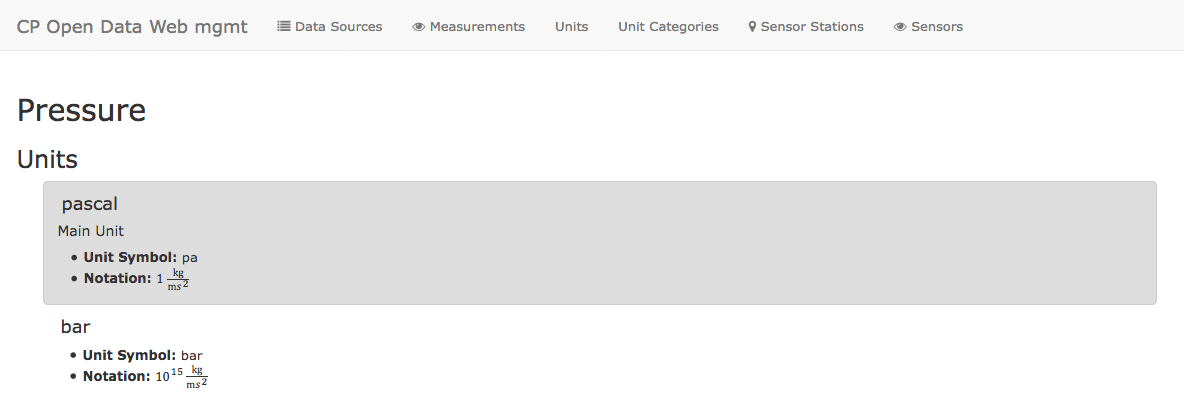
\includegraphics[width=1.00\textwidth]{images/unit_frontend.png}
	\caption{Screenshot of the units of a unit category on the web management platform. You can see the main unit and have a notation on what the units express.}
	\label{fig:screen-units}
\end{figure}

\begin{verbatim}
GET /unit_categories/:id/getMainUnit
\end{verbatim}

Example request:

\begin{verbatim}
GET /unit_categories/temperature/getMainUnit

{
    "id":"temperature_celsius",
    "name":"celsius",
    "unit_category_id":"temperature",
    "unit_symbol":"°C"
}
\end{verbatim}

\begin{verbatim}
GET /unit_categories/:id/units
\end{verbatim}

Example request:

\begin{verbatim}
GET /unit_categories/temperature/units

[
   {
      "attributes":{
         "id":"temperature_celsius",
         "name":"celsius",
         "unit_symbol":"°C",
         "unit_category_id":"temperature",
         "notation":""
      }
   },
   {
      "attributes":{
         "id":"temperature_fahrenheit",
         "name":"fahrenheit",
         "unit_symbol":"°F",
         "unit_category_id":"temperature",
         "notation":""
      }
   },
   {
      "attributes":{
         "id":"temperature_kelvin",
         "name":"kelvin",
         "unit_symbol":"K",
         "unit_category_id":"temperature",
         "notation":""
      }
   },
   ...
]
\end{verbatim}

\subsection{Discussion}\label{discussion}

As mentioned before, the planning of the extent of the functionality
offered by this system, was very vague. Besides managing metadata and
providing an API for other components, further features were at least
considered to be part of this system, like for example a scheduler that
triggers the component that handles the deployment of importers.
Therefore we chose to build this system on top of an infrastructure that
can be easily extended in many directions and has nice-to-use database
adapters instead of a more lightweight system.

While initially we also wanted to model a data source with its sensors
grouped in sensor stations, this approach would bring immense overhead
for configuring data sources in our system upfront, as a user would have
to very exactly model a data source with all its sensors and sensor
stations first. For big services like e.g.~the German Weather Service
this would be an enormous amount of work. Gathering this information
would better be done by scraping the information present in
Elasticsearch and translating them to geolocated information for all
sensors/sensor-stations/datasources. In the UML Class Diagram you can
see the modeling for this approach greyed out.

The main metainformation about the data sources (besides metadata about
the source itself) that we still needed within our system (the location
of the sensor and the grouping of sensor stations is not essential for
our system to work) and had to offer to the user registering a source
were then:

\begin{itemize}
\tightlist
\item
  Information about the measurands offered by the data source
\item
  Information about the main unit used for a measurand (see section Unit
  system)
\end{itemize}

\subsubsection{Future Improvements}\label{future-improvements}

\paragraph{Caching}

There is currently no caching solution implemented since the workloads
during development phase were quite manageable. Also including a
distributed caching system in our production pipeline seemed to be too
high of an effort and would take up significant resources that would
actually not be needed during development. We wanted, therefore, to use
the limited and expensive resources we had for actual importing.

As the number of data importers grows in production, however, requests
to the relational database would increase accordingly. Whereas scaling
the database would allow us to avoid the bottleneck, adding a cache in
front of the database to serve read requests would be sufficient to
ensure performance without incurring the cost and added complexity of
scaling. An important consideration, of course, is the frequency with
which data is updated (in our case low to none), thus making it a
perfect candidate for caching. As a distributed caching system where
read requests are very fast and possible on all nodes, Redis would be a
good fit for this use case. Writing is quite expensive due to the
replication method used by Redis, but because of the infrequent updates
to our data, we are willing to accept the trade-off in exchange for very
fast reads.

\paragraph{Exchange Scheduling information}

Due to not quite being able to reach every goal of our initial plan as
to how the architecture should look like, the scheduler had to move to
the deployment component (i.e.~the deployment to the Kubernetes
cluster). While this component should be responsible for deploying data
importers, the information about the schedule should actually be
provided to the web management system by the user. This is currently not
happening. There would be several ways how to manage scheduling and/or
deliver the scheduling information from this system to the component
handling the scheduling.

\begin{itemize}
\tightlist
\item
  Having a background processing component that acts as a scheduler
  within the web management platform. This would require an API to
  trigger the deploy on the component responsible for that, which we
  were not able to achieve.
\item
  Having a microservice-like component that is only responsible for
  scheduling and triggering importers to be deployed. This would as well
  require an API on the deployment component.
\item
  Leave the scheduling within the deployment component. This would also
  require an API, but just for receiving the general schedule, not for
  offering a hook to trigger an import.
\end{itemize}

The second option seems more granular and conforms better to our general
microservice approach but would also require the most configuration and
deployment effort. Including a scheduler in the web management platform
would somehow violate this approach but still make sense, as this
component could easily be integrated within Ruby on Rails and would be a
standalone component within it.

\section{Data Source Metadata Management System}\label{sec:metadata}

\textbf{Authoriship: } Written by Paul Wille\\
\emph{Proofread \& edited by Andres} \\

\vspace*{4mm}

In this chapter we will discuss the component responsible for managing
metadata about the data sources which are imported to the system. We
will cover what it is and does, some thoughts around why we decided to
include such a component, and how it was realized and implemented.

\subsection{Requirements}\label{requirements}

The main purpose of the component is to:

\begin{itemize}
\tightlist
\item
  serve as a registry of data sources in the system,
\item
  provide data source metadata to other components in the system,
\item
  provide users with information about units of measurement,
\item
  enable users who want to use the data to see the resources our system
  contains
\end{itemize}

In contrast to nearly every other component we had to implement, the
management platform did not have to meet as many criteria as a
distributed cloud system in general. The data it contains is quite
static and the number of requests that we expect is also quite low.
However, the following general cloud-specific architectural style
requirements were taken into consideration:

\begin{itemize}
\tightlist
\item
  Availability to other system components, that require the held
  information
\item
  Quick response time (for query optimization within the public search
  API)
\item
  Ability to run asynchronous background tasks (for scheduling)
\end{itemize}

\subsection{Implementation}\label{implementation}

The system was built using \emph{Ruby on Rails} with \emph{PostgreSQL}
as a database. The reasons why we chose to use Rails are:

\begin{itemize}
\tightlist
\item
  Relatively fast development of an MVC web application
\item
  Well established (over a decade), has therefore lots of resources ---
  also for all kinds of extensions
\item
  Extensive community support
\item
  Very good integrated ORM adapters that could easily be exchanged for
  ODM adapters for document databases
\item
  Offers the dynamic of Ruby as programming language
\end{itemize}

\subsection{Domain Model}\label{domain-model}

\begin{figure}
	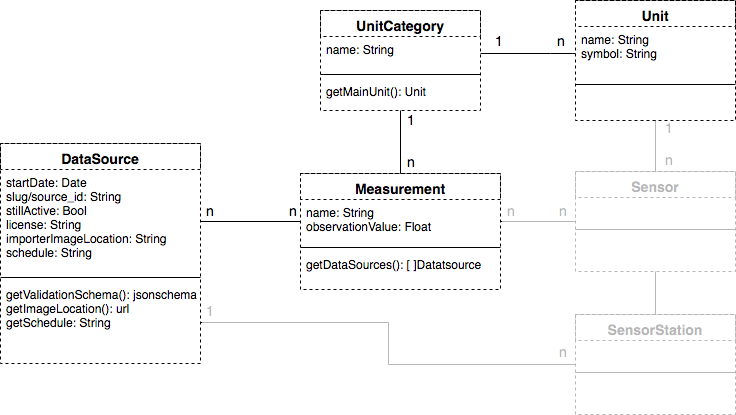
\includegraphics[width=1.00\textwidth]{images/relational_schema.png}
	\caption{UML Class Diagram of the Metadata Management System}
	\label{fig:uml-model}
\end{figure}

\subsubsection{Data Sources Registry}\label{data-sources-registry}

Before data from a given source can be imported, important information
about the source must be made available to our system. This information
consists of static metainformation and has no direct relation to actual
data being provided in the source.

We chose not to store it in the same database as the actual sensor
measurement data, but have a separate system instead. This provides
isolation between our sources and the database, preventing changes in
the choice of database or its schema from having any effect in how we
store and maintain data sources.

The metainformation that has to be provided to our system prior to
importing mainly consists of:

\begin{itemize}
\tightlist
\item
  Name of the source
\item
  Start date from which the source provides data
\item
  Whether the source is still active (i.e.~data is actively being
  provided by the source).
\item
  if not, the end date (last date for which data was provided).
\item
  Under what license the data is published
\end{itemize}

Additionally we ask the user to provide additional information, which is
useful for our system:

\begin{itemize}
\tightlist
\item
  If the data source is still active, at what schedule is new data
  published
\item
  A \emph{slug} that can be used as an id within our pipeline and in
  Elasticsearch
\item
  The measurements provided by the data source (which actual
  measurements the data source collects)
\item
  The URL location of the Docker container to be executed to import the
  data.
\end{itemize}

\begin{figure}
	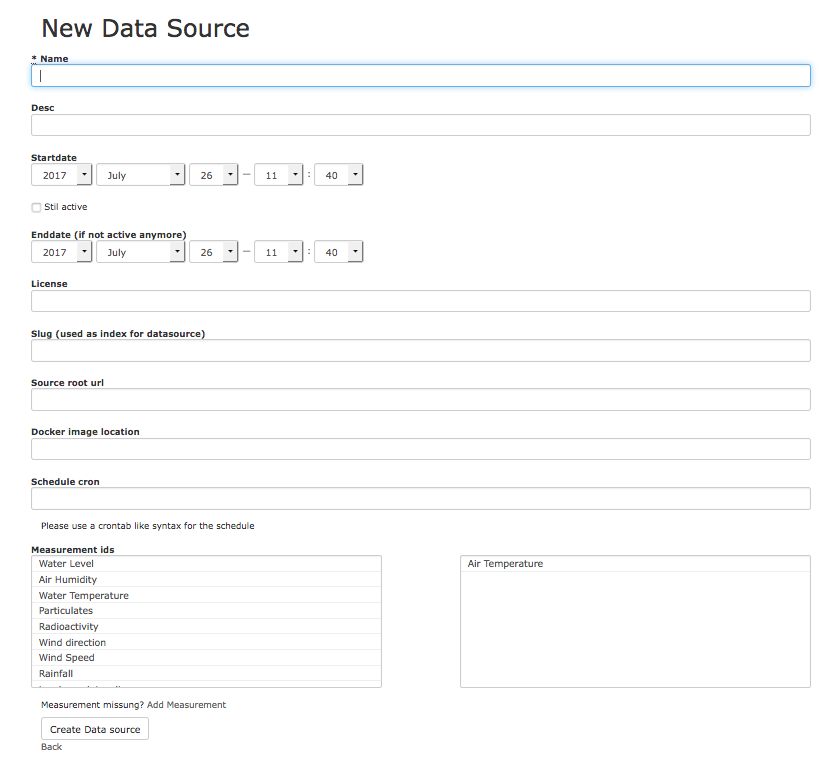
\includegraphics[width=1.00\textwidth]{images/new_datasource.png}
	\caption{Registering a data source within the Web management platform}
	\label{fig:register-source}
\end{figure}

\subsubsection{Validation Schema}\label{validation-schema}

As described in the chapter about validation and insertion into
Elasticsearch, we have a separate, distinct component that is
responsible for validating the output from data importers.

To achieve this, a schema must be provided against which to validate.
Since this schema itself is fixed, it could be hardcoded into the
validator, without the need to make another HTTP request. We decided
that this would be a bad idea for the following reasons:

\begin{itemize}
\tightlist
\item
  Sanity checks: in addition to schema-only validation, the schema
  provided by this component can validate data-source-specific values
  (such as importer IDs, etc.), which could not be validated with a
  generic validator.
\item
  Version management: schema changes over time would require changing
  the information hardcoded within the validator, and completely
  rebuilding and redeploying the validator component itself. Updating a
  record inside this component is far simpler than redeploying
  infrastructure, which is inherently more complex in an era where no
  downtime is expected.
\end{itemize}

Therefore we needed a place where said validation schema can reside. The
web management system seemed to be the right pace for that, as it
already carries metainformation about data sources and the data sources
are registered there. So it is easy to provide the relevant schema
information as well. The management system provides an API call to
supply the validation schema to the validators which looks like this:

\begin{verbatim}
GET /data_sources/:id/getValidationSchema
\end{verbatim}

The response looks like as follows (note that the const
\texttt{source\_id} would be replaced by the ID of the data source):

\begin{verbatim}
{
  "\$schema": "http://json-schema.org/schema#",
  "title": "Data Source",
  "description": "A Data Source for Open Sensor Data from the CP project \\
									at TU Berlin. ",
  "type": "object",
  "properties": {
    "source_id": {"const": "source_slug"},
    "device": {"type": "string"},
    "timestamp": { "type": "string", "format": "date-time" },
    "timestamp_data": { "type": "string", "format": "date-time" },
    "location": {
      "type": "object",
      "properties": {
        "lat": {"type": "number",
                "exclusiveMaximum": true,
                "exclusiveMinimum": true,
                "maximum": 90,
                "minimum": -90
               },
        "lon": {"type": "number",
                "exclusiveMaximum": true,
                "exclusiveMinimum": true,
                "maximum": 180,
                "minimum": -180,
               }
      },
    "required": ["lat", "lon"]
    },
    "license": {"type": "string"},
    "sensors": {
      "type": "object",
      "items": [
      {
        "type": "object",
        "properties": {
          "sensor": {"type": "string"},
          "observation_type": {"type": "string"},
          "observation_value": {"type": "number"}
        }
      }]
    }
  },
  "required": ["source_id", "timestamp","sensors", "location", "license"]
}
\end{verbatim}

\subsubsection{Provide Information to the Elasticsearch API for query
optimization}\label{provide-information-to-the-elasticsearch-api-for-query-optimization}

As described in the data model section, our model is data-source-based
and not measurand-based. For queries spanning across measurands, it will
be necessary to have further information about the relationship between
data sources and measurands.

As there were several possibilities as to where this information could
be stored and managed, and how it would be provided, the easiest place
to start with in our opinion was with the implementer of an importer,
since he or she must provide information to us when registering the data
source. The user therefore has to mark what measurements a data source
contains upfront (see Figure \ref{fig:register-source}).

In order to optimize querying, this information is provided to the API
that wraps the search interface of Elasticsearch via an API itself. The
information is stored in an indexed join table that holds the mapping
between data source and the measurands it contains. As can be seen in
the class diagram \ref{fig:uml-model} of the relational system, queries
in both directions are provided: getting all measurands for a data
source, and getting all data sources that contain a given measurand. The
corresponding routes look like this:

\begin{verbatim}
GET /data_sources/:id/measurements
\end{verbatim}

Example:

\begin{verbatim}
GET /data_sources/blume_messnetz/measurands

[
   {
      "id":1,
      "name":"Air Temperature",
      "desc":"",
      "unit_category_id":"temperature"
   },
   {
      "id":3,
      "name":"Air Humidity",
      "desc":"amount of water vapor present in the air",
      "unit_category_id":"humidity"
   }
]
\end{verbatim}

\begin{verbatim}
GET /measurements/:id/data_sources
\end{verbatim}

An example request would look like following

\begin{verbatim}
GET /measurements/1/data_sources

[
    { "id":1, "slug":"blume_messnetz", "license":"" },
    { "id":5, "slug":"german_weather_service", "license":"" }
]
\end{verbatim}

\subsubsection{Provide configuration information to the deployment
component}\label{provide-configuration-information-to-the-deployment-component}

Since the importer registration the only step in which the implementer
has to provide information to our system, it should cover all
configuration information needed to get an importer running.

\subsubsection{Units}\label{units}

With the requirements in mind, we modeled units like so:

\begin{enumerate}
\def\labelenumi{\arabic{enumi}.}
\tightlist
\item
  \textbf{Unit Categories}: Units themselves belong to a unit category.
  The unit category describes an entity for which measurements exist,
  which express their observations with one of the units of that
  category (see Figure \ref{fig:uml-model}).
\item
  Each unit has a \textbf{main unit} that we decide on. By calling the
  API or visiting the management platform a user can see, which the main
  unit is. Within our datastore we only use the main unit of a unit
  category for expressing measurements.
\item
  Units are managed by admins receptively users with permit to do so.
\item
  We therefore have a curated list of the unit categories and units
\item
  If there are units, measurements or even categories missing, each user
  can propose new ones. This proposals are also managed by the group of
  people managing the units.
\end{enumerate}

Measurements are controlled on the platform itself to allow users to
better propose new measurements, as this may happen more often. Units
and the Unit categories however are managed in a \emph{.yml} file. The
syntax we used looks like following for one entry:

\begin{verbatim}
From config/constants/units.yml:

pascal:
  id: pressure_pascal
  name: "pascal"
  unit_symbol: "pa"
  unit_category_id: pressure
  notation: "1 <centerdot>
              <mfrac>
                <mrow>
                  kg
                </mrow>
                <mrow>
                  m
                  <msup>
                          <mi>s</mi>
                          <mn>2</mn>
                </mrow>
              </mfrac>"

From config/constants/unit_categories.yml:

pressure:
  id: pressure
  name: Pressure
\end{verbatim}

The unit categories are pretty straightforward. For a unit there are
some more possibilities. Besides declaring the unit symbol, the category
it belongs to, its name you are allowed to use MathML to express what
the meaning of a unit is. This is especially helpful with units that can
be directly converted to each other (Figure \ref{fig:screen-units}).

The API of the web management system also provides calls to a) receive
the main unit of a unit category and to b) get a list of all units there
are for a unit category. Both of these information are of course aswell
accessible from the frontend of the system.

\begin{figure}[b]
	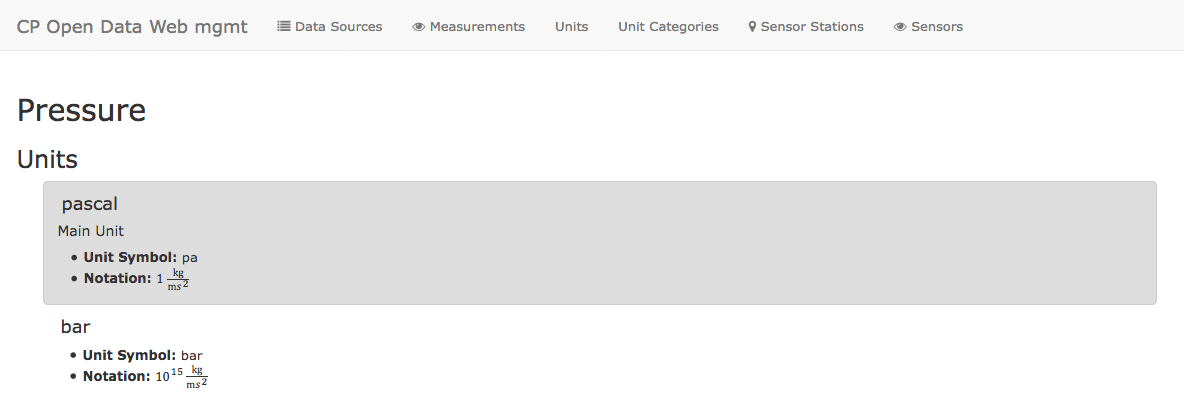
\includegraphics[width=1.00\textwidth]{images/unit_frontend.png}
	\caption{Screenshot of the units of a unit category on the web management platform. You can see the main unit and have a notation on what the units express.}
	\label{fig:screen-units}
\end{figure}

\begin{verbatim}
GET /unit_categories/:id/getMainUnit
\end{verbatim}

Example request:

\begin{verbatim}
GET /unit_categories/temperature/getMainUnit

{
    "id":"temperature_celsius",
    "name":"celsius",
    "unit_category_id":"temperature",
    "unit_symbol":"°C"
}
\end{verbatim}

\begin{verbatim}
GET /unit_categories/:id/units
\end{verbatim}

Example request:

\begin{verbatim}
GET /unit_categories/temperature/units

[
   {
      "attributes":{
         "id":"temperature_celsius",
         "name":"celsius",
         "unit_symbol":"°C",
         "unit_category_id":"temperature",
         "notation":""
      }
   },
   {
      "attributes":{
         "id":"temperature_fahrenheit",
         "name":"fahrenheit",
         "unit_symbol":"°F",
         "unit_category_id":"temperature",
         "notation":""
      }
   },
   {
      "attributes":{
         "id":"temperature_kelvin",
         "name":"kelvin",
         "unit_symbol":"K",
         "unit_category_id":"temperature",
         "notation":""
      }
   },
   ...
]
\end{verbatim}

\subsection{Discussion}\label{discussion}

As mentioned before, the planning of the extent of the functionality
offered by this system, was very vague. Besides managing metadata and
providing an API for other components, further features were at least
considered to be part of this system, like for example a scheduler that
triggers the component that handles the deployment of importers.
Therefore we chose to build this system on top of an infrastructure that
can be easily extended in many directions and has nice-to-use database
adapters instead of a more lightweight system.

While initially we also wanted to model a data source with its sensors
grouped in sensor stations, this approach would bring immense overhead
for configuring data sources in our system upfront, as a user would have
to very exactly model a data source with all its sensors and sensor
stations first. For big services like e.g.~the German Weather Service
this would be an enormous amount of work. Gathering this information
would better be done by scraping the information present in
Elasticsearch and translating them to geolocated information for all
sensors/sensor-stations/datasources. In the UML Class Diagram you can
see the modeling for this approach greyed out.

The main metainformation about the data sources (besides metadata about
the source itself) that we still needed within our system (the location
of the sensor and the grouping of sensor stations is not essential for
our system to work) and had to offer to the user registering a source
were then:

\begin{itemize}
\tightlist
\item
  Information about the measurands offered by the data source
\item
  Information about the main unit used for a measurand (see section Unit
  system)
\end{itemize}

\subsubsection{Future Improvements}\label{future-improvements}

\paragraph{Caching}

There is currently no caching solution implemented since the workloads
during development phase were quite manageable. Also including a
distributed caching system in our production pipeline seemed to be too
high of an effort and would take up significant resources that would
actually not be needed during development. We wanted, therefore, to use
the limited and expensive resources we had for actual importing.

As the number of data importers grows in production, however, requests
to the relational database would increase accordingly. Whereas scaling
the database would allow us to avoid the bottleneck, adding a cache in
front of the database to serve read requests would be sufficient to
ensure performance without incurring the cost and added complexity of
scaling. An important consideration, of course, is the frequency with
which data is updated (in our case low to none), thus making it a
perfect candidate for caching. As a distributed caching system where
read requests are very fast and possible on all nodes, Redis would be a
good fit for this use case. Writing is quite expensive due to the
replication method used by Redis, but because of the infrequent updates
to our data, we are willing to accept the trade-off in exchange for very
fast reads.

\paragraph{Exchange Scheduling information}

Due to not quite being able to reach every goal of our initial plan as
to how the architecture should look like, the scheduler had to move to
the deployment component (i.e.~the deployment to the Kubernetes
cluster). While this component should be responsible for deploying data
importers, the information about the schedule should actually be
provided to the web management system by the user. This is currently not
happening. There would be several ways how to manage scheduling and/or
deliver the scheduling information from this system to the component
handling the scheduling.

\begin{itemize}
\tightlist
\item
  Having a background processing component that acts as a scheduler
  within the web management platform. This would require an API to
  trigger the deploy on the component responsible for that, which we
  were not able to achieve.
\item
  Having a microservice-like component that is only responsible for
  scheduling and triggering importers to be deployed. This would as well
  require an API on the deployment component.
\item
  Leave the scheduling within the deployment component. This would also
  require an API, but just for receiving the general schedule, not for
  offering a hook to trigger an import.
\end{itemize}

The second option seems more granular and conforms better to our general
microservice approach but would also require the most configuration and
deployment effort. Including a scheduler in the web management platform
would somehow violate this approach but still make sense, as this
component could easily be integrated within Ruby on Rails and would be a
standalone component within it.

\section{Data Source Metadata Management System}\label{sec:metadata}

\textbf{Authoriship: } Written by Paul Wille\\
\emph{Proofread \& edited by Andres} \\

\vspace*{4mm}

In this chapter we will discuss the component responsible for managing
metadata about the data sources which are imported to the system. We
will cover what it is and does, some thoughts around why we decided to
include such a component, and how it was realized and implemented.

\subsection{Requirements}\label{requirements}

The main purpose of the component is to:

\begin{itemize}
\tightlist
\item
  serve as a registry of data sources in the system,
\item
  provide data source metadata to other components in the system,
\item
  provide users with information about units of measurement,
\item
  enable users who want to use the data to see the resources our system
  contains
\end{itemize}

In contrast to nearly every other component we had to implement, the
management platform did not have to meet as many criteria as a
distributed cloud system in general. The data it contains is quite
static and the number of requests that we expect is also quite low.
However, the following general cloud-specific architectural style
requirements were taken into consideration:

\begin{itemize}
\tightlist
\item
  Availability to other system components, that require the held
  information
\item
  Quick response time (for query optimization within the public search
  API)
\item
  Ability to run asynchronous background tasks (for scheduling)
\end{itemize}

\subsection{Implementation}\label{implementation}

The system was built using \emph{Ruby on Rails} with \emph{PostgreSQL}
as a database. The reasons why we chose to use Rails are:

\begin{itemize}
\tightlist
\item
  Relatively fast development of an MVC web application
\item
  Well established (over a decade), has therefore lots of resources ---
  also for all kinds of extensions
\item
  Extensive community support
\item
  Very good integrated ORM adapters that could easily be exchanged for
  ODM adapters for document databases
\item
  Offers the dynamic of Ruby as programming language
\end{itemize}

\subsection{Domain Model}\label{domain-model}

\begin{figure}
	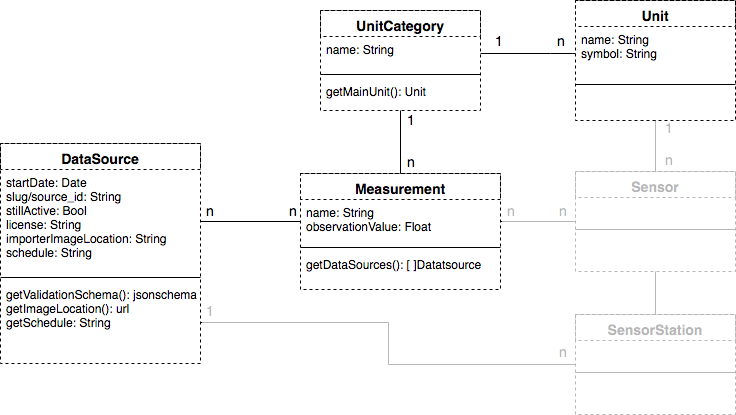
\includegraphics[width=1.00\textwidth]{images/relational_schema.png}
	\caption{UML Class Diagram of the Metadata Management System}
	\label{fig:uml-model}
\end{figure}

\subsubsection{Data Sources Registry}\label{data-sources-registry}

Before data from a given source can be imported, important information
about the source must be made available to our system. This information
consists of static metainformation and has no direct relation to actual
data being provided in the source.

We chose not to store it in the same database as the actual sensor
measurement data, but have a separate system instead. This provides
isolation between our sources and the database, preventing changes in
the choice of database or its schema from having any effect in how we
store and maintain data sources.

The metainformation that has to be provided to our system prior to
importing mainly consists of:

\begin{itemize}
\tightlist
\item
  Name of the source
\item
  Start date from which the source provides data
\item
  Whether the source is still active (i.e.~data is actively being
  provided by the source).
\item
  if not, the end date (last date for which data was provided).
\item
  Under what license the data is published
\end{itemize}

Additionally we ask the user to provide additional information, which is
useful for our system:

\begin{itemize}
\tightlist
\item
  If the data source is still active, at what schedule is new data
  published
\item
  A \emph{slug} that can be used as an id within our pipeline and in
  Elasticsearch
\item
  The measurements provided by the data source (which actual
  measurements the data source collects)
\item
  The URL location of the Docker container to be executed to import the
  data.
\end{itemize}

\begin{figure}
	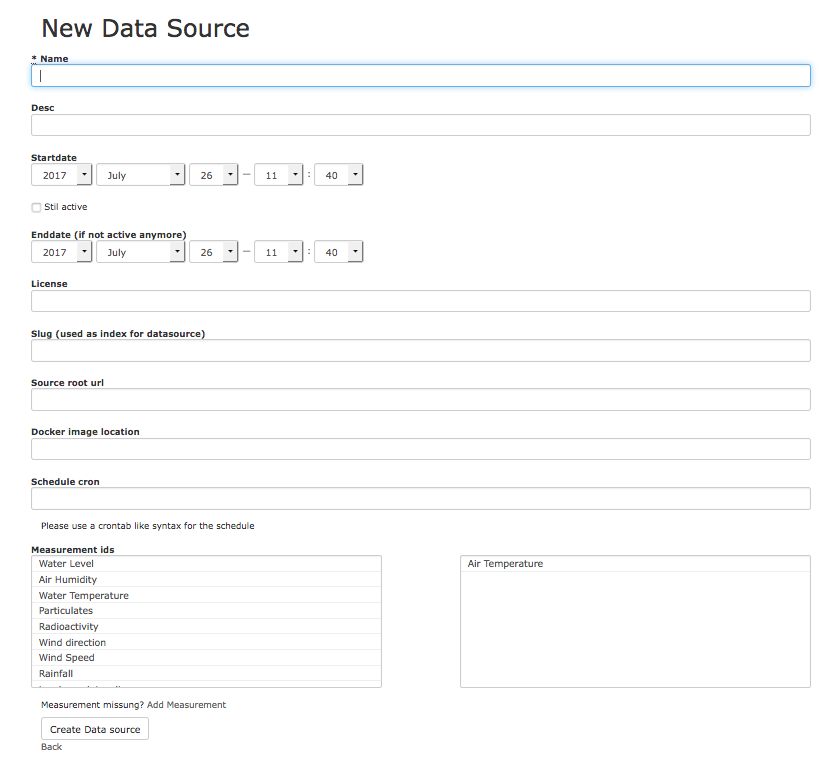
\includegraphics[width=1.00\textwidth]{images/new_datasource.png}
	\caption{Registering a data source within the Web management platform}
	\label{fig:register-source}
\end{figure}

\subsubsection{Validation Schema}\label{validation-schema}

As described in the chapter about validation and insertion into
Elasticsearch, we have a separate, distinct component that is
responsible for validating the output from data importers.

To achieve this, a schema must be provided against which to validate.
Since this schema itself is fixed, it could be hardcoded into the
validator, without the need to make another HTTP request. We decided
that this would be a bad idea for the following reasons:

\begin{itemize}
\tightlist
\item
  Sanity checks: in addition to schema-only validation, the schema
  provided by this component can validate data-source-specific values
  (such as importer IDs, etc.), which could not be validated with a
  generic validator.
\item
  Version management: schema changes over time would require changing
  the information hardcoded within the validator, and completely
  rebuilding and redeploying the validator component itself. Updating a
  record inside this component is far simpler than redeploying
  infrastructure, which is inherently more complex in an era where no
  downtime is expected.
\end{itemize}

Therefore we needed a place where said validation schema can reside. The
web management system seemed to be the right pace for that, as it
already carries metainformation about data sources and the data sources
are registered there. So it is easy to provide the relevant schema
information as well. The management system provides an API call to
supply the validation schema to the validators which looks like this:

\begin{verbatim}
GET /data_sources/:id/getValidationSchema
\end{verbatim}

The response looks like as follows (note that the const
\texttt{source\_id} would be replaced by the ID of the data source):

\begin{verbatim}
{
  "\$schema": "http://json-schema.org/schema#",
  "title": "Data Source",
  "description": "A Data Source for Open Sensor Data from the CP project \\
									at TU Berlin. ",
  "type": "object",
  "properties": {
    "source_id": {"const": "source_slug"},
    "device": {"type": "string"},
    "timestamp": { "type": "string", "format": "date-time" },
    "timestamp_data": { "type": "string", "format": "date-time" },
    "location": {
      "type": "object",
      "properties": {
        "lat": {"type": "number",
                "exclusiveMaximum": true,
                "exclusiveMinimum": true,
                "maximum": 90,
                "minimum": -90
               },
        "lon": {"type": "number",
                "exclusiveMaximum": true,
                "exclusiveMinimum": true,
                "maximum": 180,
                "minimum": -180,
               }
      },
    "required": ["lat", "lon"]
    },
    "license": {"type": "string"},
    "sensors": {
      "type": "object",
      "items": [
      {
        "type": "object",
        "properties": {
          "sensor": {"type": "string"},
          "observation_type": {"type": "string"},
          "observation_value": {"type": "number"}
        }
      }]
    }
  },
  "required": ["source_id", "timestamp","sensors", "location", "license"]
}
\end{verbatim}

\subsubsection{Provide Information to the Elasticsearch API for query
optimization}\label{provide-information-to-the-elasticsearch-api-for-query-optimization}

As described in the data model section, our model is data-source-based
and not measurand-based. For queries spanning across measurands, it will
be necessary to have further information about the relationship between
data sources and measurands.

As there were several possibilities as to where this information could
be stored and managed, and how it would be provided, the easiest place
to start with in our opinion was with the implementer of an importer,
since he or she must provide information to us when registering the data
source. The user therefore has to mark what measurements a data source
contains upfront (see Figure \ref{fig:register-source}).

In order to optimize querying, this information is provided to the API
that wraps the search interface of Elasticsearch via an API itself. The
information is stored in an indexed join table that holds the mapping
between data source and the measurands it contains. As can be seen in
the class diagram \ref{fig:uml-model} of the relational system, queries
in both directions are provided: getting all measurands for a data
source, and getting all data sources that contain a given measurand. The
corresponding routes look like this:

\begin{verbatim}
GET /data_sources/:id/measurements
\end{verbatim}

Example:

\begin{verbatim}
GET /data_sources/blume_messnetz/measurands

[
   {
      "id":1,
      "name":"Air Temperature",
      "desc":"",
      "unit_category_id":"temperature"
   },
   {
      "id":3,
      "name":"Air Humidity",
      "desc":"amount of water vapor present in the air",
      "unit_category_id":"humidity"
   }
]
\end{verbatim}

\begin{verbatim}
GET /measurements/:id/data_sources
\end{verbatim}

An example request would look like following

\begin{verbatim}
GET /measurements/1/data_sources

[
    { "id":1, "slug":"blume_messnetz", "license":"" },
    { "id":5, "slug":"german_weather_service", "license":"" }
]
\end{verbatim}

\subsubsection{Provide configuration information to the deployment
component}\label{provide-configuration-information-to-the-deployment-component}

Since the importer registration the only step in which the implementer
has to provide information to our system, it should cover all
configuration information needed to get an importer running.

\subsubsection{Units}\label{units}

With the requirements in mind, we modeled units like so:

\begin{enumerate}
\def\labelenumi{\arabic{enumi}.}
\tightlist
\item
  \textbf{Unit Categories}: Units themselves belong to a unit category.
  The unit category describes an entity for which measurements exist,
  which express their observations with one of the units of that
  category (see Figure \ref{fig:uml-model}).
\item
  Each unit has a \textbf{main unit} that we decide on. By calling the
  API or visiting the management platform a user can see, which the main
  unit is. Within our datastore we only use the main unit of a unit
  category for expressing measurements.
\item
  Units are managed by admins receptively users with permit to do so.
\item
  We therefore have a curated list of the unit categories and units
\item
  If there are units, measurements or even categories missing, each user
  can propose new ones. This proposals are also managed by the group of
  people managing the units.
\end{enumerate}

Measurements are controlled on the platform itself to allow users to
better propose new measurements, as this may happen more often. Units
and the Unit categories however are managed in a \emph{.yml} file. The
syntax we used looks like following for one entry:

\begin{verbatim}
From config/constants/units.yml:

pascal:
  id: pressure_pascal
  name: "pascal"
  unit_symbol: "pa"
  unit_category_id: pressure
  notation: "1 <centerdot>
              <mfrac>
                <mrow>
                  kg
                </mrow>
                <mrow>
                  m
                  <msup>
                          <mi>s</mi>
                          <mn>2</mn>
                </mrow>
              </mfrac>"

From config/constants/unit_categories.yml:

pressure:
  id: pressure
  name: Pressure
\end{verbatim}

The unit categories are pretty straightforward. For a unit there are
some more possibilities. Besides declaring the unit symbol, the category
it belongs to, its name you are allowed to use MathML to express what
the meaning of a unit is. This is especially helpful with units that can
be directly converted to each other (Figure \ref{fig:screen-units}).

The API of the web management system also provides calls to a) receive
the main unit of a unit category and to b) get a list of all units there
are for a unit category. Both of these information are of course aswell
accessible from the frontend of the system.

\begin{figure}[b]
	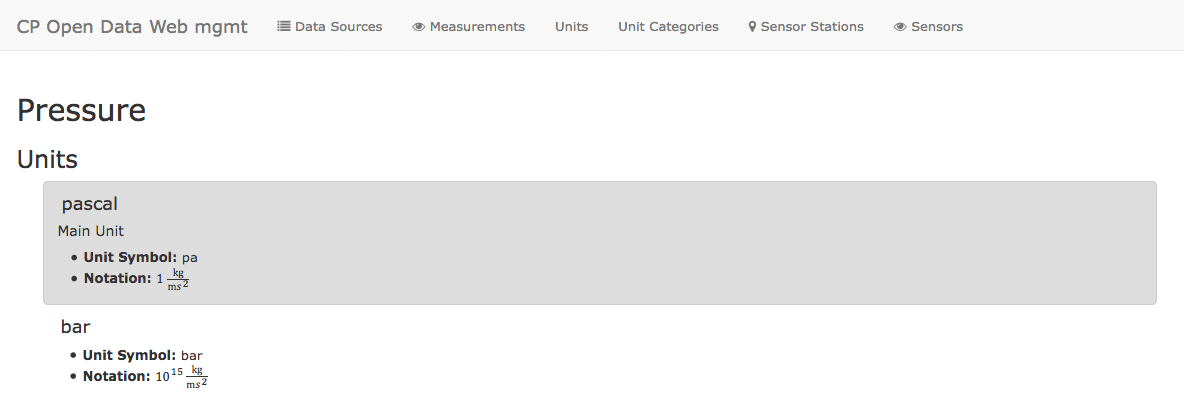
\includegraphics[width=1.00\textwidth]{images/unit_frontend.png}
	\caption{Screenshot of the units of a unit category on the web management platform. You can see the main unit and have a notation on what the units express.}
	\label{fig:screen-units}
\end{figure}

\begin{verbatim}
GET /unit_categories/:id/getMainUnit
\end{verbatim}

Example request:

\begin{verbatim}
GET /unit_categories/temperature/getMainUnit

{
    "id":"temperature_celsius",
    "name":"celsius",
    "unit_category_id":"temperature",
    "unit_symbol":"°C"
}
\end{verbatim}

\begin{verbatim}
GET /unit_categories/:id/units
\end{verbatim}

Example request:

\begin{verbatim}
GET /unit_categories/temperature/units

[
   {
      "attributes":{
         "id":"temperature_celsius",
         "name":"celsius",
         "unit_symbol":"°C",
         "unit_category_id":"temperature",
         "notation":""
      }
   },
   {
      "attributes":{
         "id":"temperature_fahrenheit",
         "name":"fahrenheit",
         "unit_symbol":"°F",
         "unit_category_id":"temperature",
         "notation":""
      }
   },
   {
      "attributes":{
         "id":"temperature_kelvin",
         "name":"kelvin",
         "unit_symbol":"K",
         "unit_category_id":"temperature",
         "notation":""
      }
   },
   ...
]
\end{verbatim}

\subsection{Discussion}\label{discussion}

As mentioned before, the planning of the extent of the functionality
offered by this system, was very vague. Besides managing metadata and
providing an API for other components, further features were at least
considered to be part of this system, like for example a scheduler that
triggers the component that handles the deployment of importers.
Therefore we chose to build this system on top of an infrastructure that
can be easily extended in many directions and has nice-to-use database
adapters instead of a more lightweight system.

While initially we also wanted to model a data source with its sensors
grouped in sensor stations, this approach would bring immense overhead
for configuring data sources in our system upfront, as a user would have
to very exactly model a data source with all its sensors and sensor
stations first. For big services like e.g.~the German Weather Service
this would be an enormous amount of work. Gathering this information
would better be done by scraping the information present in
Elasticsearch and translating them to geolocated information for all
sensors/sensor-stations/datasources. In the UML Class Diagram you can
see the modeling for this approach greyed out.

The main metainformation about the data sources (besides metadata about
the source itself) that we still needed within our system (the location
of the sensor and the grouping of sensor stations is not essential for
our system to work) and had to offer to the user registering a source
were then:

\begin{itemize}
\tightlist
\item
  Information about the measurands offered by the data source
\item
  Information about the main unit used for a measurand (see section Unit
  system)
\end{itemize}

\subsubsection{Future Improvements}\label{future-improvements}

\paragraph{Caching}

There is currently no caching solution implemented since the workloads
during development phase were quite manageable. Also including a
distributed caching system in our production pipeline seemed to be too
high of an effort and would take up significant resources that would
actually not be needed during development. We wanted, therefore, to use
the limited and expensive resources we had for actual importing.

As the number of data importers grows in production, however, requests
to the relational database would increase accordingly. Whereas scaling
the database would allow us to avoid the bottleneck, adding a cache in
front of the database to serve read requests would be sufficient to
ensure performance without incurring the cost and added complexity of
scaling. An important consideration, of course, is the frequency with
which data is updated (in our case low to none), thus making it a
perfect candidate for caching. As a distributed caching system where
read requests are very fast and possible on all nodes, Redis would be a
good fit for this use case. Writing is quite expensive due to the
replication method used by Redis, but because of the infrequent updates
to our data, we are willing to accept the trade-off in exchange for very
fast reads.

\paragraph{Exchange Scheduling information}

Due to not quite being able to reach every goal of our initial plan as
to how the architecture should look like, the scheduler had to move to
the deployment component (i.e.~the deployment to the Kubernetes
cluster). While this component should be responsible for deploying data
importers, the information about the schedule should actually be
provided to the web management system by the user. This is currently not
happening. There would be several ways how to manage scheduling and/or
deliver the scheduling information from this system to the component
handling the scheduling.

\begin{itemize}
\tightlist
\item
  Having a background processing component that acts as a scheduler
  within the web management platform. This would require an API to
  trigger the deploy on the component responsible for that, which we
  were not able to achieve.
\item
  Having a microservice-like component that is only responsible for
  scheduling and triggering importers to be deployed. This would as well
  require an API on the deployment component.
\item
  Leave the scheduling within the deployment component. This would also
  require an API, but just for receiving the general schedule, not for
  offering a hook to trigger an import.
\end{itemize}

The second option seems more granular and conforms better to our general
microservice approach but would also require the most configuration and
deployment effort. Including a scheduler in the web management platform
would somehow violate this approach but still make sense, as this
component could easily be integrated within Ruby on Rails and would be a
standalone component within it.

\section{Data Source Metadata Management System}\label{sec:metadata}

\textbf{Authoriship: } Written by Paul Wille\\
\emph{Proofread \& edited by Andres} \\

\vspace*{4mm}

In this chapter we will discuss the component responsible for managing
metadata about the data sources which are imported to the system. We
will cover what it is and does, some thoughts around why we decided to
include such a component, and how it was realized and implemented.

\subsection{Requirements}\label{requirements}

The main purpose of the component is to:

\begin{itemize}
\tightlist
\item
  serve as a registry of data sources in the system,
\item
  provide data source metadata to other components in the system,
\item
  provide users with information about units of measurement,
\item
  enable users who want to use the data to see the resources our system
  contains
\end{itemize}

In contrast to nearly every other component we had to implement, the
management platform did not have to meet as many criteria as a
distributed cloud system in general. The data it contains is quite
static and the number of requests that we expect is also quite low.
However, the following general cloud-specific architectural style
requirements were taken into consideration:

\begin{itemize}
\tightlist
\item
  Availability to other system components, that require the held
  information
\item
  Quick response time (for query optimization within the public search
  API)
\item
  Ability to run asynchronous background tasks (for scheduling)
\end{itemize}

\subsection{Implementation}\label{implementation}

The system was built using \emph{Ruby on Rails} with \emph{PostgreSQL}
as a database. The reasons why we chose to use Rails are:

\begin{itemize}
\tightlist
\item
  Relatively fast development of an MVC web application
\item
  Well established (over a decade), has therefore lots of resources ---
  also for all kinds of extensions
\item
  Extensive community support
\item
  Very good integrated ORM adapters that could easily be exchanged for
  ODM adapters for document databases
\item
  Offers the dynamic of Ruby as programming language
\end{itemize}

\subsection{Domain Model}\label{domain-model}

\begin{figure}
	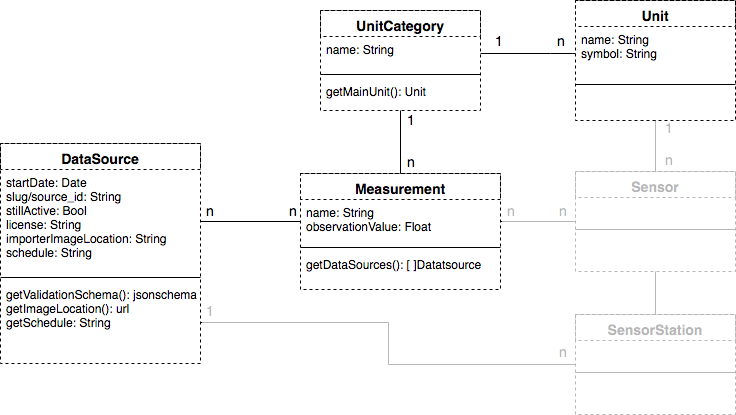
\includegraphics[width=1.00\textwidth]{images/relational_schema.png}
	\caption{UML Class Diagram of the Metadata Management System}
	\label{fig:uml-model}
\end{figure}

\subsubsection{Data Sources Registry}\label{data-sources-registry}

Before data from a given source can be imported, important information
about the source must be made available to our system. This information
consists of static metainformation and has no direct relation to actual
data being provided in the source.

We chose not to store it in the same database as the actual sensor
measurement data, but have a separate system instead. This provides
isolation between our sources and the database, preventing changes in
the choice of database or its schema from having any effect in how we
store and maintain data sources.

The metainformation that has to be provided to our system prior to
importing mainly consists of:

\begin{itemize}
\tightlist
\item
  Name of the source
\item
  Start date from which the source provides data
\item
  Whether the source is still active (i.e.~data is actively being
  provided by the source).
\item
  if not, the end date (last date for which data was provided).
\item
  Under what license the data is published
\end{itemize}

Additionally we ask the user to provide additional information, which is
useful for our system:

\begin{itemize}
\tightlist
\item
  If the data source is still active, at what schedule is new data
  published
\item
  A \emph{slug} that can be used as an id within our pipeline and in
  Elasticsearch
\item
  The measurements provided by the data source (which actual
  measurements the data source collects)
\item
  The URL location of the Docker container to be executed to import the
  data.
\end{itemize}

\begin{figure}
	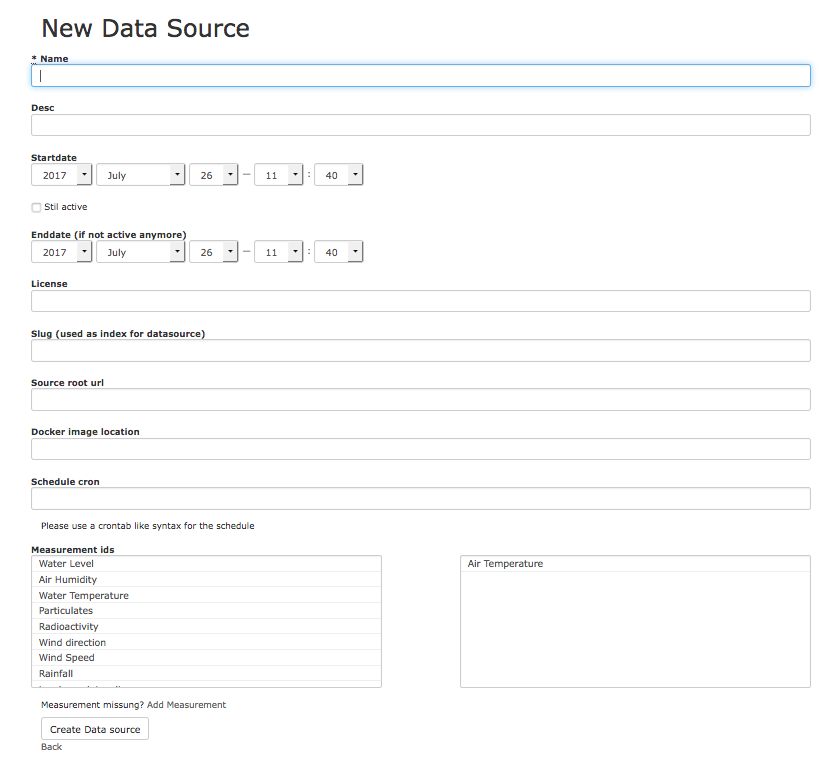
\includegraphics[width=1.00\textwidth]{images/new_datasource.png}
	\caption{Registering a data source within the Web management platform}
	\label{fig:register-source}
\end{figure}

\subsubsection{Validation Schema}\label{validation-schema}

As described in the chapter about validation and insertion into
Elasticsearch, we have a separate, distinct component that is
responsible for validating the output from data importers.

To achieve this, a schema must be provided against which to validate.
Since this schema itself is fixed, it could be hardcoded into the
validator, without the need to make another HTTP request. We decided
that this would be a bad idea for the following reasons:

\begin{itemize}
\tightlist
\item
  Sanity checks: in addition to schema-only validation, the schema
  provided by this component can validate data-source-specific values
  (such as importer IDs, etc.), which could not be validated with a
  generic validator.
\item
  Version management: schema changes over time would require changing
  the information hardcoded within the validator, and completely
  rebuilding and redeploying the validator component itself. Updating a
  record inside this component is far simpler than redeploying
  infrastructure, which is inherently more complex in an era where no
  downtime is expected.
\end{itemize}

Therefore we needed a place where said validation schema can reside. The
web management system seemed to be the right pace for that, as it
already carries metainformation about data sources and the data sources
are registered there. So it is easy to provide the relevant schema
information as well. The management system provides an API call to
supply the validation schema to the validators which looks like this:

\begin{verbatim}
GET /data_sources/:id/getValidationSchema
\end{verbatim}

The response looks like as follows (note that the const
\texttt{source\_id} would be replaced by the ID of the data source):

\begin{verbatim}
{
  "\$schema": "http://json-schema.org/schema#",
  "title": "Data Source",
  "description": "A Data Source for Open Sensor Data from the CP project \\
									at TU Berlin. ",
  "type": "object",
  "properties": {
    "source_id": {"const": "source_slug"},
    "device": {"type": "string"},
    "timestamp": { "type": "string", "format": "date-time" },
    "timestamp_data": { "type": "string", "format": "date-time" },
    "location": {
      "type": "object",
      "properties": {
        "lat": {"type": "number",
                "exclusiveMaximum": true,
                "exclusiveMinimum": true,
                "maximum": 90,
                "minimum": -90
               },
        "lon": {"type": "number",
                "exclusiveMaximum": true,
                "exclusiveMinimum": true,
                "maximum": 180,
                "minimum": -180,
               }
      },
    "required": ["lat", "lon"]
    },
    "license": {"type": "string"},
    "sensors": {
      "type": "object",
      "items": [
      {
        "type": "object",
        "properties": {
          "sensor": {"type": "string"},
          "observation_type": {"type": "string"},
          "observation_value": {"type": "number"}
        }
      }]
    }
  },
  "required": ["source_id", "timestamp","sensors", "location", "license"]
}
\end{verbatim}

\subsubsection{Provide Information to the Elasticsearch API for query
optimization}\label{provide-information-to-the-elasticsearch-api-for-query-optimization}

As described in the data model section, our model is data-source-based
and not measurand-based. For queries spanning across measurands, it will
be necessary to have further information about the relationship between
data sources and measurands.

As there were several possibilities as to where this information could
be stored and managed, and how it would be provided, the easiest place
to start with in our opinion was with the implementer of an importer,
since he or she must provide information to us when registering the data
source. The user therefore has to mark what measurements a data source
contains upfront (see Figure \ref{fig:register-source}).

In order to optimize querying, this information is provided to the API
that wraps the search interface of Elasticsearch via an API itself. The
information is stored in an indexed join table that holds the mapping
between data source and the measurands it contains. As can be seen in
the class diagram \ref{fig:uml-model} of the relational system, queries
in both directions are provided: getting all measurands for a data
source, and getting all data sources that contain a given measurand. The
corresponding routes look like this:

\begin{verbatim}
GET /data_sources/:id/measurements
\end{verbatim}

Example:

\begin{verbatim}
GET /data_sources/blume_messnetz/measurands

[
   {
      "id":1,
      "name":"Air Temperature",
      "desc":"",
      "unit_category_id":"temperature"
   },
   {
      "id":3,
      "name":"Air Humidity",
      "desc":"amount of water vapor present in the air",
      "unit_category_id":"humidity"
   }
]
\end{verbatim}

\begin{verbatim}
GET /measurements/:id/data_sources
\end{verbatim}

An example request would look like following

\begin{verbatim}
GET /measurements/1/data_sources

[
    { "id":1, "slug":"blume_messnetz", "license":"" },
    { "id":5, "slug":"german_weather_service", "license":"" }
]
\end{verbatim}

\subsubsection{Provide configuration information to the deployment
component}\label{provide-configuration-information-to-the-deployment-component}

Since the importer registration the only step in which the implementer
has to provide information to our system, it should cover all
configuration information needed to get an importer running.

\subsubsection{Units}\label{units}

With the requirements in mind, we modeled units like so:

\begin{enumerate}
\def\labelenumi{\arabic{enumi}.}
\tightlist
\item
  \textbf{Unit Categories}: Units themselves belong to a unit category.
  The unit category describes an entity for which measurements exist,
  which express their observations with one of the units of that
  category (see Figure \ref{fig:uml-model}).
\item
  Each unit has a \textbf{main unit} that we decide on. By calling the
  API or visiting the management platform a user can see, which the main
  unit is. Within our datastore we only use the main unit of a unit
  category for expressing measurements.
\item
  Units are managed by admins receptively users with permit to do so.
\item
  We therefore have a curated list of the unit categories and units
\item
  If there are units, measurements or even categories missing, each user
  can propose new ones. This proposals are also managed by the group of
  people managing the units.
\end{enumerate}

Measurements are controlled on the platform itself to allow users to
better propose new measurements, as this may happen more often. Units
and the Unit categories however are managed in a \emph{.yml} file. The
syntax we used looks like following for one entry:

\begin{verbatim}
From config/constants/units.yml:

pascal:
  id: pressure_pascal
  name: "pascal"
  unit_symbol: "pa"
  unit_category_id: pressure
  notation: "1 <centerdot>
              <mfrac>
                <mrow>
                  kg
                </mrow>
                <mrow>
                  m
                  <msup>
                          <mi>s</mi>
                          <mn>2</mn>
                </mrow>
              </mfrac>"

From config/constants/unit_categories.yml:

pressure:
  id: pressure
  name: Pressure
\end{verbatim}

The unit categories are pretty straightforward. For a unit there are
some more possibilities. Besides declaring the unit symbol, the category
it belongs to, its name you are allowed to use MathML to express what
the meaning of a unit is. This is especially helpful with units that can
be directly converted to each other (Figure \ref{fig:screen-units}).

The API of the web management system also provides calls to a) receive
the main unit of a unit category and to b) get a list of all units there
are for a unit category. Both of these information are of course aswell
accessible from the frontend of the system.

\begin{figure}[b]
	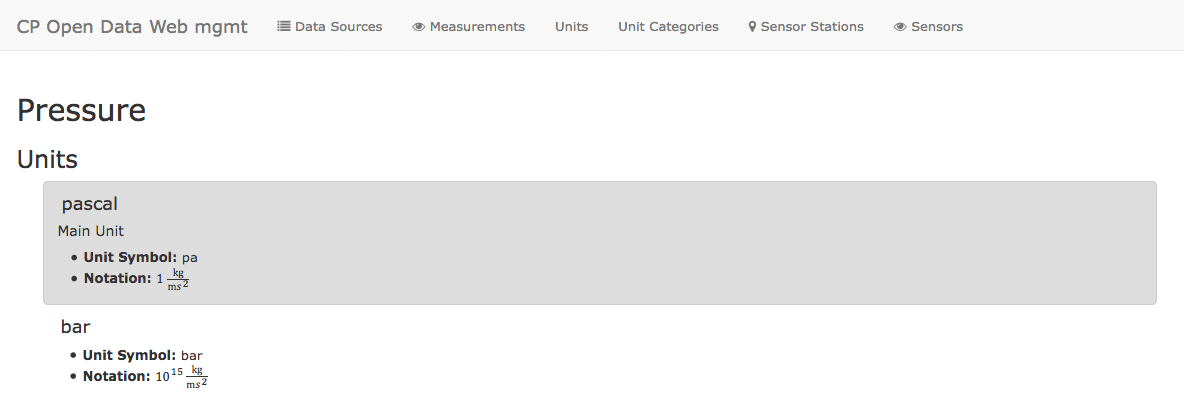
\includegraphics[width=1.00\textwidth]{images/unit_frontend.png}
	\caption{Screenshot of the units of a unit category on the web management platform. You can see the main unit and have a notation on what the units express.}
	\label{fig:screen-units}
\end{figure}

\begin{verbatim}
GET /unit_categories/:id/getMainUnit
\end{verbatim}

Example request:

\begin{verbatim}
GET /unit_categories/temperature/getMainUnit

{
    "id":"temperature_celsius",
    "name":"celsius",
    "unit_category_id":"temperature",
    "unit_symbol":"°C"
}
\end{verbatim}

\begin{verbatim}
GET /unit_categories/:id/units
\end{verbatim}

Example request:

\begin{verbatim}
GET /unit_categories/temperature/units

[
   {
      "attributes":{
         "id":"temperature_celsius",
         "name":"celsius",
         "unit_symbol":"°C",
         "unit_category_id":"temperature",
         "notation":""
      }
   },
   {
      "attributes":{
         "id":"temperature_fahrenheit",
         "name":"fahrenheit",
         "unit_symbol":"°F",
         "unit_category_id":"temperature",
         "notation":""
      }
   },
   {
      "attributes":{
         "id":"temperature_kelvin",
         "name":"kelvin",
         "unit_symbol":"K",
         "unit_category_id":"temperature",
         "notation":""
      }
   },
   ...
]
\end{verbatim}

\subsection{Discussion}\label{discussion}

As mentioned before, the planning of the extent of the functionality
offered by this system, was very vague. Besides managing metadata and
providing an API for other components, further features were at least
considered to be part of this system, like for example a scheduler that
triggers the component that handles the deployment of importers.
Therefore we chose to build this system on top of an infrastructure that
can be easily extended in many directions and has nice-to-use database
adapters instead of a more lightweight system.

While initially we also wanted to model a data source with its sensors
grouped in sensor stations, this approach would bring immense overhead
for configuring data sources in our system upfront, as a user would have
to very exactly model a data source with all its sensors and sensor
stations first. For big services like e.g.~the German Weather Service
this would be an enormous amount of work. Gathering this information
would better be done by scraping the information present in
Elasticsearch and translating them to geolocated information for all
sensors/sensor-stations/datasources. In the UML Class Diagram you can
see the modeling for this approach greyed out.

The main metainformation about the data sources (besides metadata about
the source itself) that we still needed within our system (the location
of the sensor and the grouping of sensor stations is not essential for
our system to work) and had to offer to the user registering a source
were then:

\begin{itemize}
\tightlist
\item
  Information about the measurands offered by the data source
\item
  Information about the main unit used for a measurand (see section Unit
  system)
\end{itemize}

\subsubsection{Future Improvements}\label{future-improvements}

\paragraph{Caching}

There is currently no caching solution implemented since the workloads
during development phase were quite manageable. Also including a
distributed caching system in our production pipeline seemed to be too
high of an effort and would take up significant resources that would
actually not be needed during development. We wanted, therefore, to use
the limited and expensive resources we had for actual importing.

As the number of data importers grows in production, however, requests
to the relational database would increase accordingly. Whereas scaling
the database would allow us to avoid the bottleneck, adding a cache in
front of the database to serve read requests would be sufficient to
ensure performance without incurring the cost and added complexity of
scaling. An important consideration, of course, is the frequency with
which data is updated (in our case low to none), thus making it a
perfect candidate for caching. As a distributed caching system where
read requests are very fast and possible on all nodes, Redis would be a
good fit for this use case. Writing is quite expensive due to the
replication method used by Redis, but because of the infrequent updates
to our data, we are willing to accept the trade-off in exchange for very
fast reads.

\paragraph{Exchange Scheduling information}

Due to not quite being able to reach every goal of our initial plan as
to how the architecture should look like, the scheduler had to move to
the deployment component (i.e.~the deployment to the Kubernetes
cluster). While this component should be responsible for deploying data
importers, the information about the schedule should actually be
provided to the web management system by the user. This is currently not
happening. There would be several ways how to manage scheduling and/or
deliver the scheduling information from this system to the component
handling the scheduling.

\begin{itemize}
\tightlist
\item
  Having a background processing component that acts as a scheduler
  within the web management platform. This would require an API to
  trigger the deploy on the component responsible for that, which we
  were not able to achieve.
\item
  Having a microservice-like component that is only responsible for
  scheduling and triggering importers to be deployed. This would as well
  require an API on the deployment component.
\item
  Leave the scheduling within the deployment component. This would also
  require an API, but just for receiving the general schedule, not for
  offering a hook to trigger an import.
\end{itemize}

The second option seems more granular and conforms better to our general
microservice approach but would also require the most configuration and
deployment effort. Including a scheduler in the web management platform
would somehow violate this approach but still make sense, as this
component could easily be integrated within Ruby on Rails and would be a
standalone component within it.

%\section{Data Source Metadata Management System}\label{sec:metadata}

\textbf{Authoriship: } Written by Paul Wille\\
\emph{Proofread \& edited by Andres} \\

\vspace*{4mm}

In this chapter we will discuss the component responsible for managing
metadata about the data sources which are imported to the system. We
will cover what it is and does, some thoughts around why we decided to
include such a component, and how it was realized and implemented.

\subsection{Requirements}\label{requirements}

The main purpose of the component is to:

\begin{itemize}
\tightlist
\item
  serve as a registry of data sources in the system,
\item
  provide data source metadata to other components in the system,
\item
  provide users with information about units of measurement,
\item
  enable users who want to use the data to see the resources our system
  contains
\end{itemize}

In contrast to nearly every other component we had to implement, the
management platform did not have to meet as many criteria as a
distributed cloud system in general. The data it contains is quite
static and the number of requests that we expect is also quite low.
However, the following general cloud-specific architectural style
requirements were taken into consideration:

\begin{itemize}
\tightlist
\item
  Availability to other system components, that require the held
  information
\item
  Quick response time (for query optimization within the public search
  API)
\item
  Ability to run asynchronous background tasks (for scheduling)
\end{itemize}

\subsection{Implementation}\label{implementation}

The system was built using \emph{Ruby on Rails} with \emph{PostgreSQL}
as a database. The reasons why we chose to use Rails are:

\begin{itemize}
\tightlist
\item
  Relatively fast development of an MVC web application
\item
  Well established (over a decade), has therefore lots of resources ---
  also for all kinds of extensions
\item
  Extensive community support
\item
  Very good integrated ORM adapters that could easily be exchanged for
  ODM adapters for document databases
\item
  Offers the dynamic of Ruby as programming language
\end{itemize}

\subsection{Domain Model}\label{domain-model}

\begin{figure}
	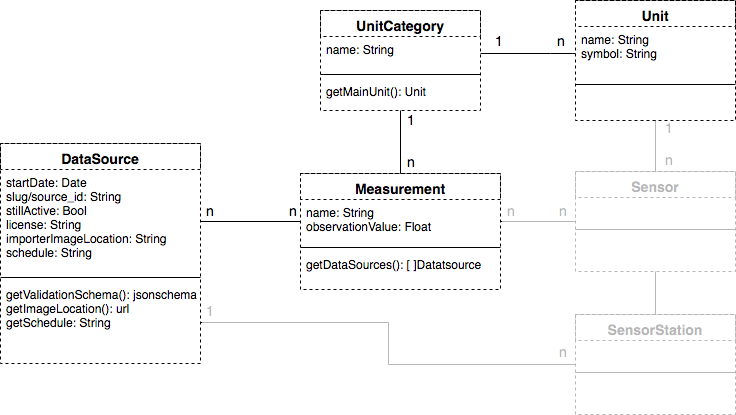
\includegraphics[width=1.00\textwidth]{images/relational_schema.png}
	\caption{UML Class Diagram of the Metadata Management System}
	\label{fig:uml-model}
\end{figure}

\subsubsection{Data Sources Registry}\label{data-sources-registry}

Before data from a given source can be imported, important information
about the source must be made available to our system. This information
consists of static metainformation and has no direct relation to actual
data being provided in the source.

We chose not to store it in the same database as the actual sensor
measurement data, but have a separate system instead. This provides
isolation between our sources and the database, preventing changes in
the choice of database or its schema from having any effect in how we
store and maintain data sources.

The metainformation that has to be provided to our system prior to
importing mainly consists of:

\begin{itemize}
\tightlist
\item
  Name of the source
\item
  Start date from which the source provides data
\item
  Whether the source is still active (i.e.~data is actively being
  provided by the source).
\item
  if not, the end date (last date for which data was provided).
\item
  Under what license the data is published
\end{itemize}

Additionally we ask the user to provide additional information, which is
useful for our system:

\begin{itemize}
\tightlist
\item
  If the data source is still active, at what schedule is new data
  published
\item
  A \emph{slug} that can be used as an id within our pipeline and in
  Elasticsearch
\item
  The measurements provided by the data source (which actual
  measurements the data source collects)
\item
  The URL location of the Docker container to be executed to import the
  data.
\end{itemize}

\begin{figure}
	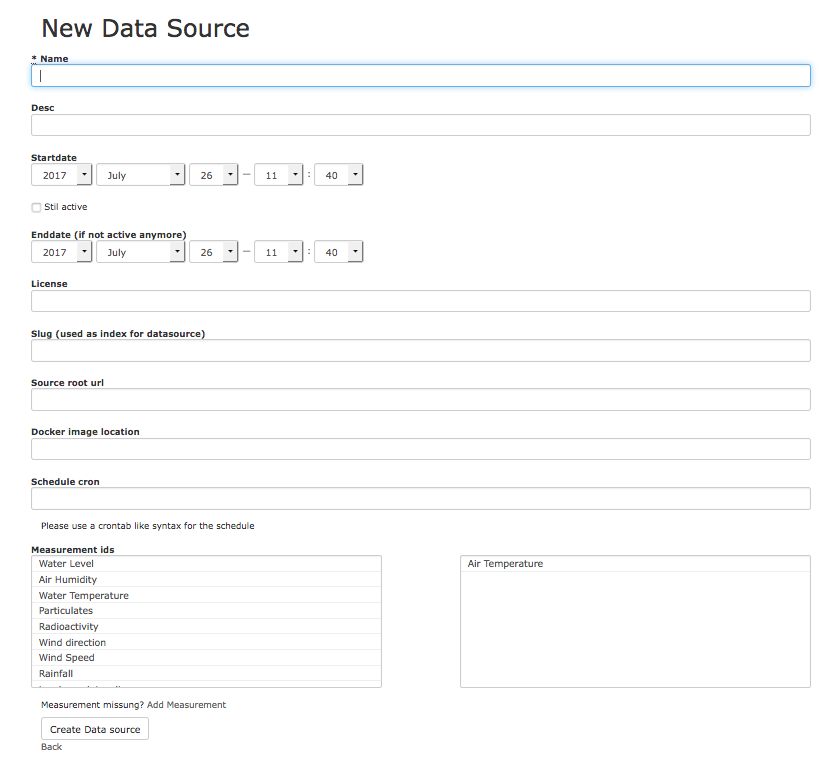
\includegraphics[width=1.00\textwidth]{images/new_datasource.png}
	\caption{Registering a data source within the Web management platform}
	\label{fig:register-source}
\end{figure}

\subsubsection{Validation Schema}\label{validation-schema}

As described in the chapter about validation and insertion into
Elasticsearch, we have a separate, distinct component that is
responsible for validating the output from data importers.

To achieve this, a schema must be provided against which to validate.
Since this schema itself is fixed, it could be hardcoded into the
validator, without the need to make another HTTP request. We decided
that this would be a bad idea for the following reasons:

\begin{itemize}
\tightlist
\item
  Sanity checks: in addition to schema-only validation, the schema
  provided by this component can validate data-source-specific values
  (such as importer IDs, etc.), which could not be validated with a
  generic validator.
\item
  Version management: schema changes over time would require changing
  the information hardcoded within the validator, and completely
  rebuilding and redeploying the validator component itself. Updating a
  record inside this component is far simpler than redeploying
  infrastructure, which is inherently more complex in an era where no
  downtime is expected.
\end{itemize}

Therefore we needed a place where said validation schema can reside. The
web management system seemed to be the right pace for that, as it
already carries metainformation about data sources and the data sources
are registered there. So it is easy to provide the relevant schema
information as well. The management system provides an API call to
supply the validation schema to the validators which looks like this:

\begin{verbatim}
GET /data_sources/:id/getValidationSchema
\end{verbatim}

The response looks like as follows (note that the const
\texttt{source\_id} would be replaced by the ID of the data source):

\begin{verbatim}
{
  "\$schema": "http://json-schema.org/schema#",
  "title": "Data Source",
  "description": "A Data Source for Open Sensor Data from the CP project \\
									at TU Berlin. ",
  "type": "object",
  "properties": {
    "source_id": {"const": "source_slug"},
    "device": {"type": "string"},
    "timestamp": { "type": "string", "format": "date-time" },
    "timestamp_data": { "type": "string", "format": "date-time" },
    "location": {
      "type": "object",
      "properties": {
        "lat": {"type": "number",
                "exclusiveMaximum": true,
                "exclusiveMinimum": true,
                "maximum": 90,
                "minimum": -90
               },
        "lon": {"type": "number",
                "exclusiveMaximum": true,
                "exclusiveMinimum": true,
                "maximum": 180,
                "minimum": -180,
               }
      },
    "required": ["lat", "lon"]
    },
    "license": {"type": "string"},
    "sensors": {
      "type": "object",
      "items": [
      {
        "type": "object",
        "properties": {
          "sensor": {"type": "string"},
          "observation_type": {"type": "string"},
          "observation_value": {"type": "number"}
        }
      }]
    }
  },
  "required": ["source_id", "timestamp","sensors", "location", "license"]
}
\end{verbatim}

\subsubsection{Provide Information to the Elasticsearch API for query
optimization}\label{provide-information-to-the-elasticsearch-api-for-query-optimization}

As described in the data model section, our model is data-source-based
and not measurand-based. For queries spanning across measurands, it will
be necessary to have further information about the relationship between
data sources and measurands.

As there were several possibilities as to where this information could
be stored and managed, and how it would be provided, the easiest place
to start with in our opinion was with the implementer of an importer,
since he or she must provide information to us when registering the data
source. The user therefore has to mark what measurements a data source
contains upfront (see Figure \ref{fig:register-source}).

In order to optimize querying, this information is provided to the API
that wraps the search interface of Elasticsearch via an API itself. The
information is stored in an indexed join table that holds the mapping
between data source and the measurands it contains. As can be seen in
the class diagram \ref{fig:uml-model} of the relational system, queries
in both directions are provided: getting all measurands for a data
source, and getting all data sources that contain a given measurand. The
corresponding routes look like this:

\begin{verbatim}
GET /data_sources/:id/measurements
\end{verbatim}

Example:

\begin{verbatim}
GET /data_sources/blume_messnetz/measurands

[
   {
      "id":1,
      "name":"Air Temperature",
      "desc":"",
      "unit_category_id":"temperature"
   },
   {
      "id":3,
      "name":"Air Humidity",
      "desc":"amount of water vapor present in the air",
      "unit_category_id":"humidity"
   }
]
\end{verbatim}

\begin{verbatim}
GET /measurements/:id/data_sources
\end{verbatim}

An example request would look like following

\begin{verbatim}
GET /measurements/1/data_sources

[
    { "id":1, "slug":"blume_messnetz", "license":"" },
    { "id":5, "slug":"german_weather_service", "license":"" }
]
\end{verbatim}

\subsubsection{Provide configuration information to the deployment
component}\label{provide-configuration-information-to-the-deployment-component}

Since the importer registration the only step in which the implementer
has to provide information to our system, it should cover all
configuration information needed to get an importer running.

\subsubsection{Units}\label{units}

With the requirements in mind, we modeled units like so:

\begin{enumerate}
\def\labelenumi{\arabic{enumi}.}
\tightlist
\item
  \textbf{Unit Categories}: Units themselves belong to a unit category.
  The unit category describes an entity for which measurements exist,
  which express their observations with one of the units of that
  category (see Figure \ref{fig:uml-model}).
\item
  Each unit has a \textbf{main unit} that we decide on. By calling the
  API or visiting the management platform a user can see, which the main
  unit is. Within our datastore we only use the main unit of a unit
  category for expressing measurements.
\item
  Units are managed by admins receptively users with permit to do so.
\item
  We therefore have a curated list of the unit categories and units
\item
  If there are units, measurements or even categories missing, each user
  can propose new ones. This proposals are also managed by the group of
  people managing the units.
\end{enumerate}

Measurements are controlled on the platform itself to allow users to
better propose new measurements, as this may happen more often. Units
and the Unit categories however are managed in a \emph{.yml} file. The
syntax we used looks like following for one entry:

\begin{verbatim}
From config/constants/units.yml:

pascal:
  id: pressure_pascal
  name: "pascal"
  unit_symbol: "pa"
  unit_category_id: pressure
  notation: "1 <centerdot>
              <mfrac>
                <mrow>
                  kg
                </mrow>
                <mrow>
                  m
                  <msup>
                          <mi>s</mi>
                          <mn>2</mn>
                </mrow>
              </mfrac>"

From config/constants/unit_categories.yml:

pressure:
  id: pressure
  name: Pressure
\end{verbatim}

The unit categories are pretty straightforward. For a unit there are
some more possibilities. Besides declaring the unit symbol, the category
it belongs to, its name you are allowed to use MathML to express what
the meaning of a unit is. This is especially helpful with units that can
be directly converted to each other (Figure \ref{fig:screen-units}).

The API of the web management system also provides calls to a) receive
the main unit of a unit category and to b) get a list of all units there
are for a unit category. Both of these information are of course aswell
accessible from the frontend of the system.

\begin{figure}[b]
	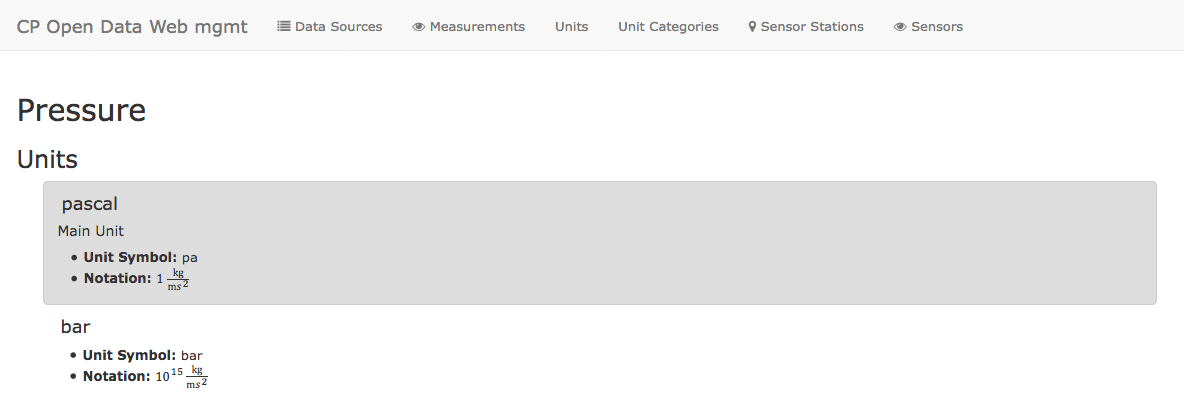
\includegraphics[width=1.00\textwidth]{images/unit_frontend.png}
	\caption{Screenshot of the units of a unit category on the web management platform. You can see the main unit and have a notation on what the units express.}
	\label{fig:screen-units}
\end{figure}

\begin{verbatim}
GET /unit_categories/:id/getMainUnit
\end{verbatim}

Example request:

\begin{verbatim}
GET /unit_categories/temperature/getMainUnit

{
    "id":"temperature_celsius",
    "name":"celsius",
    "unit_category_id":"temperature",
    "unit_symbol":"°C"
}
\end{verbatim}

\begin{verbatim}
GET /unit_categories/:id/units
\end{verbatim}

Example request:

\begin{verbatim}
GET /unit_categories/temperature/units

[
   {
      "attributes":{
         "id":"temperature_celsius",
         "name":"celsius",
         "unit_symbol":"°C",
         "unit_category_id":"temperature",
         "notation":""
      }
   },
   {
      "attributes":{
         "id":"temperature_fahrenheit",
         "name":"fahrenheit",
         "unit_symbol":"°F",
         "unit_category_id":"temperature",
         "notation":""
      }
   },
   {
      "attributes":{
         "id":"temperature_kelvin",
         "name":"kelvin",
         "unit_symbol":"K",
         "unit_category_id":"temperature",
         "notation":""
      }
   },
   ...
]
\end{verbatim}

\subsection{Discussion}\label{discussion}

As mentioned before, the planning of the extent of the functionality
offered by this system, was very vague. Besides managing metadata and
providing an API for other components, further features were at least
considered to be part of this system, like for example a scheduler that
triggers the component that handles the deployment of importers.
Therefore we chose to build this system on top of an infrastructure that
can be easily extended in many directions and has nice-to-use database
adapters instead of a more lightweight system.

While initially we also wanted to model a data source with its sensors
grouped in sensor stations, this approach would bring immense overhead
for configuring data sources in our system upfront, as a user would have
to very exactly model a data source with all its sensors and sensor
stations first. For big services like e.g.~the German Weather Service
this would be an enormous amount of work. Gathering this information
would better be done by scraping the information present in
Elasticsearch and translating them to geolocated information for all
sensors/sensor-stations/datasources. In the UML Class Diagram you can
see the modeling for this approach greyed out.

The main metainformation about the data sources (besides metadata about
the source itself) that we still needed within our system (the location
of the sensor and the grouping of sensor stations is not essential for
our system to work) and had to offer to the user registering a source
were then:

\begin{itemize}
\tightlist
\item
  Information about the measurands offered by the data source
\item
  Information about the main unit used for a measurand (see section Unit
  system)
\end{itemize}

\subsubsection{Future Improvements}\label{future-improvements}

\paragraph{Caching}

There is currently no caching solution implemented since the workloads
during development phase were quite manageable. Also including a
distributed caching system in our production pipeline seemed to be too
high of an effort and would take up significant resources that would
actually not be needed during development. We wanted, therefore, to use
the limited and expensive resources we had for actual importing.

As the number of data importers grows in production, however, requests
to the relational database would increase accordingly. Whereas scaling
the database would allow us to avoid the bottleneck, adding a cache in
front of the database to serve read requests would be sufficient to
ensure performance without incurring the cost and added complexity of
scaling. An important consideration, of course, is the frequency with
which data is updated (in our case low to none), thus making it a
perfect candidate for caching. As a distributed caching system where
read requests are very fast and possible on all nodes, Redis would be a
good fit for this use case. Writing is quite expensive due to the
replication method used by Redis, but because of the infrequent updates
to our data, we are willing to accept the trade-off in exchange for very
fast reads.

\paragraph{Exchange Scheduling information}

Due to not quite being able to reach every goal of our initial plan as
to how the architecture should look like, the scheduler had to move to
the deployment component (i.e.~the deployment to the Kubernetes
cluster). While this component should be responsible for deploying data
importers, the information about the schedule should actually be
provided to the web management system by the user. This is currently not
happening. There would be several ways how to manage scheduling and/or
deliver the scheduling information from this system to the component
handling the scheduling.

\begin{itemize}
\tightlist
\item
  Having a background processing component that acts as a scheduler
  within the web management platform. This would require an API to
  trigger the deploy on the component responsible for that, which we
  were not able to achieve.
\item
  Having a microservice-like component that is only responsible for
  scheduling and triggering importers to be deployed. This would as well
  require an API on the deployment component.
\item
  Leave the scheduling within the deployment component. This would also
  require an API, but just for receiving the general schedule, not for
  offering a hook to trigger an import.
\end{itemize}

The second option seems more granular and conforms better to our general
microservice approach but would also require the most configuration and
deployment effort. Including a scheduler in the web management platform
would somehow violate this approach but still make sense, as this
component could easily be integrated within Ruby on Rails and would be a
standalone component within it.

%\section{Data Source Metadata Management System}\label{sec:metadata}

\textbf{Authoriship: } Written by Paul Wille\\
\emph{Proofread \& edited by Andres} \\

\vspace*{4mm}

In this chapter we will discuss the component responsible for managing
metadata about the data sources which are imported to the system. We
will cover what it is and does, some thoughts around why we decided to
include such a component, and how it was realized and implemented.

\subsection{Requirements}\label{requirements}

The main purpose of the component is to:

\begin{itemize}
\tightlist
\item
  serve as a registry of data sources in the system,
\item
  provide data source metadata to other components in the system,
\item
  provide users with information about units of measurement,
\item
  enable users who want to use the data to see the resources our system
  contains
\end{itemize}

In contrast to nearly every other component we had to implement, the
management platform did not have to meet as many criteria as a
distributed cloud system in general. The data it contains is quite
static and the number of requests that we expect is also quite low.
However, the following general cloud-specific architectural style
requirements were taken into consideration:

\begin{itemize}
\tightlist
\item
  Availability to other system components, that require the held
  information
\item
  Quick response time (for query optimization within the public search
  API)
\item
  Ability to run asynchronous background tasks (for scheduling)
\end{itemize}

\subsection{Implementation}\label{implementation}

The system was built using \emph{Ruby on Rails} with \emph{PostgreSQL}
as a database. The reasons why we chose to use Rails are:

\begin{itemize}
\tightlist
\item
  Relatively fast development of an MVC web application
\item
  Well established (over a decade), has therefore lots of resources ---
  also for all kinds of extensions
\item
  Extensive community support
\item
  Very good integrated ORM adapters that could easily be exchanged for
  ODM adapters for document databases
\item
  Offers the dynamic of Ruby as programming language
\end{itemize}

\subsection{Domain Model}\label{domain-model}

\begin{figure}
	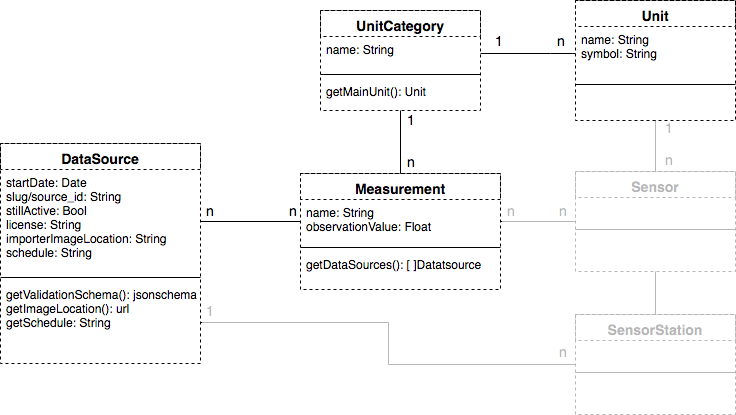
\includegraphics[width=1.00\textwidth]{images/relational_schema.png}
	\caption{UML Class Diagram of the Metadata Management System}
	\label{fig:uml-model}
\end{figure}

\subsubsection{Data Sources Registry}\label{data-sources-registry}

Before data from a given source can be imported, important information
about the source must be made available to our system. This information
consists of static metainformation and has no direct relation to actual
data being provided in the source.

We chose not to store it in the same database as the actual sensor
measurement data, but have a separate system instead. This provides
isolation between our sources and the database, preventing changes in
the choice of database or its schema from having any effect in how we
store and maintain data sources.

The metainformation that has to be provided to our system prior to
importing mainly consists of:

\begin{itemize}
\tightlist
\item
  Name of the source
\item
  Start date from which the source provides data
\item
  Whether the source is still active (i.e.~data is actively being
  provided by the source).
\item
  if not, the end date (last date for which data was provided).
\item
  Under what license the data is published
\end{itemize}

Additionally we ask the user to provide additional information, which is
useful for our system:

\begin{itemize}
\tightlist
\item
  If the data source is still active, at what schedule is new data
  published
\item
  A \emph{slug} that can be used as an id within our pipeline and in
  Elasticsearch
\item
  The measurements provided by the data source (which actual
  measurements the data source collects)
\item
  The URL location of the Docker container to be executed to import the
  data.
\end{itemize}

\begin{figure}
	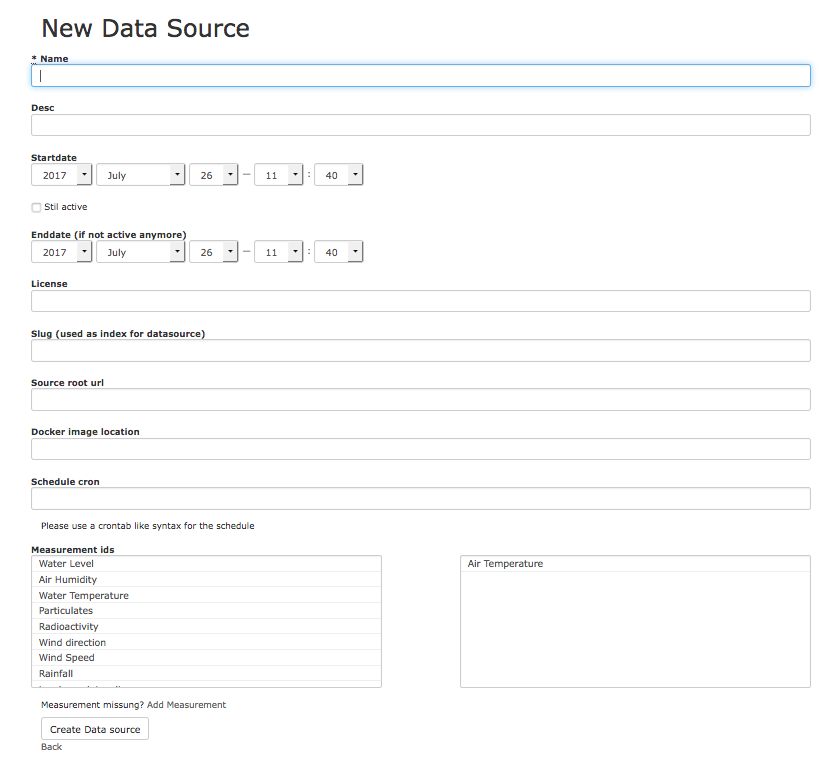
\includegraphics[width=1.00\textwidth]{images/new_datasource.png}
	\caption{Registering a data source within the Web management platform}
	\label{fig:register-source}
\end{figure}

\subsubsection{Validation Schema}\label{validation-schema}

As described in the chapter about validation and insertion into
Elasticsearch, we have a separate, distinct component that is
responsible for validating the output from data importers.

To achieve this, a schema must be provided against which to validate.
Since this schema itself is fixed, it could be hardcoded into the
validator, without the need to make another HTTP request. We decided
that this would be a bad idea for the following reasons:

\begin{itemize}
\tightlist
\item
  Sanity checks: in addition to schema-only validation, the schema
  provided by this component can validate data-source-specific values
  (such as importer IDs, etc.), which could not be validated with a
  generic validator.
\item
  Version management: schema changes over time would require changing
  the information hardcoded within the validator, and completely
  rebuilding and redeploying the validator component itself. Updating a
  record inside this component is far simpler than redeploying
  infrastructure, which is inherently more complex in an era where no
  downtime is expected.
\end{itemize}

Therefore we needed a place where said validation schema can reside. The
web management system seemed to be the right pace for that, as it
already carries metainformation about data sources and the data sources
are registered there. So it is easy to provide the relevant schema
information as well. The management system provides an API call to
supply the validation schema to the validators which looks like this:

\begin{verbatim}
GET /data_sources/:id/getValidationSchema
\end{verbatim}

The response looks like as follows (note that the const
\texttt{source\_id} would be replaced by the ID of the data source):

\begin{verbatim}
{
  "\$schema": "http://json-schema.org/schema#",
  "title": "Data Source",
  "description": "A Data Source for Open Sensor Data from the CP project \\
									at TU Berlin. ",
  "type": "object",
  "properties": {
    "source_id": {"const": "source_slug"},
    "device": {"type": "string"},
    "timestamp": { "type": "string", "format": "date-time" },
    "timestamp_data": { "type": "string", "format": "date-time" },
    "location": {
      "type": "object",
      "properties": {
        "lat": {"type": "number",
                "exclusiveMaximum": true,
                "exclusiveMinimum": true,
                "maximum": 90,
                "minimum": -90
               },
        "lon": {"type": "number",
                "exclusiveMaximum": true,
                "exclusiveMinimum": true,
                "maximum": 180,
                "minimum": -180,
               }
      },
    "required": ["lat", "lon"]
    },
    "license": {"type": "string"},
    "sensors": {
      "type": "object",
      "items": [
      {
        "type": "object",
        "properties": {
          "sensor": {"type": "string"},
          "observation_type": {"type": "string"},
          "observation_value": {"type": "number"}
        }
      }]
    }
  },
  "required": ["source_id", "timestamp","sensors", "location", "license"]
}
\end{verbatim}

\subsubsection{Provide Information to the Elasticsearch API for query
optimization}\label{provide-information-to-the-elasticsearch-api-for-query-optimization}

As described in the data model section, our model is data-source-based
and not measurand-based. For queries spanning across measurands, it will
be necessary to have further information about the relationship between
data sources and measurands.

As there were several possibilities as to where this information could
be stored and managed, and how it would be provided, the easiest place
to start with in our opinion was with the implementer of an importer,
since he or she must provide information to us when registering the data
source. The user therefore has to mark what measurements a data source
contains upfront (see Figure \ref{fig:register-source}).

In order to optimize querying, this information is provided to the API
that wraps the search interface of Elasticsearch via an API itself. The
information is stored in an indexed join table that holds the mapping
between data source and the measurands it contains. As can be seen in
the class diagram \ref{fig:uml-model} of the relational system, queries
in both directions are provided: getting all measurands for a data
source, and getting all data sources that contain a given measurand. The
corresponding routes look like this:

\begin{verbatim}
GET /data_sources/:id/measurements
\end{verbatim}

Example:

\begin{verbatim}
GET /data_sources/blume_messnetz/measurands

[
   {
      "id":1,
      "name":"Air Temperature",
      "desc":"",
      "unit_category_id":"temperature"
   },
   {
      "id":3,
      "name":"Air Humidity",
      "desc":"amount of water vapor present in the air",
      "unit_category_id":"humidity"
   }
]
\end{verbatim}

\begin{verbatim}
GET /measurements/:id/data_sources
\end{verbatim}

An example request would look like following

\begin{verbatim}
GET /measurements/1/data_sources

[
    { "id":1, "slug":"blume_messnetz", "license":"" },
    { "id":5, "slug":"german_weather_service", "license":"" }
]
\end{verbatim}

\subsubsection{Provide configuration information to the deployment
component}\label{provide-configuration-information-to-the-deployment-component}

Since the importer registration the only step in which the implementer
has to provide information to our system, it should cover all
configuration information needed to get an importer running.

\subsubsection{Units}\label{units}

With the requirements in mind, we modeled units like so:

\begin{enumerate}
\def\labelenumi{\arabic{enumi}.}
\tightlist
\item
  \textbf{Unit Categories}: Units themselves belong to a unit category.
  The unit category describes an entity for which measurements exist,
  which express their observations with one of the units of that
  category (see Figure \ref{fig:uml-model}).
\item
  Each unit has a \textbf{main unit} that we decide on. By calling the
  API or visiting the management platform a user can see, which the main
  unit is. Within our datastore we only use the main unit of a unit
  category for expressing measurements.
\item
  Units are managed by admins receptively users with permit to do so.
\item
  We therefore have a curated list of the unit categories and units
\item
  If there are units, measurements or even categories missing, each user
  can propose new ones. This proposals are also managed by the group of
  people managing the units.
\end{enumerate}

Measurements are controlled on the platform itself to allow users to
better propose new measurements, as this may happen more often. Units
and the Unit categories however are managed in a \emph{.yml} file. The
syntax we used looks like following for one entry:

\begin{verbatim}
From config/constants/units.yml:

pascal:
  id: pressure_pascal
  name: "pascal"
  unit_symbol: "pa"
  unit_category_id: pressure
  notation: "1 <centerdot>
              <mfrac>
                <mrow>
                  kg
                </mrow>
                <mrow>
                  m
                  <msup>
                          <mi>s</mi>
                          <mn>2</mn>
                </mrow>
              </mfrac>"

From config/constants/unit_categories.yml:

pressure:
  id: pressure
  name: Pressure
\end{verbatim}

The unit categories are pretty straightforward. For a unit there are
some more possibilities. Besides declaring the unit symbol, the category
it belongs to, its name you are allowed to use MathML to express what
the meaning of a unit is. This is especially helpful with units that can
be directly converted to each other (Figure \ref{fig:screen-units}).

The API of the web management system also provides calls to a) receive
the main unit of a unit category and to b) get a list of all units there
are for a unit category. Both of these information are of course aswell
accessible from the frontend of the system.

\begin{figure}[b]
	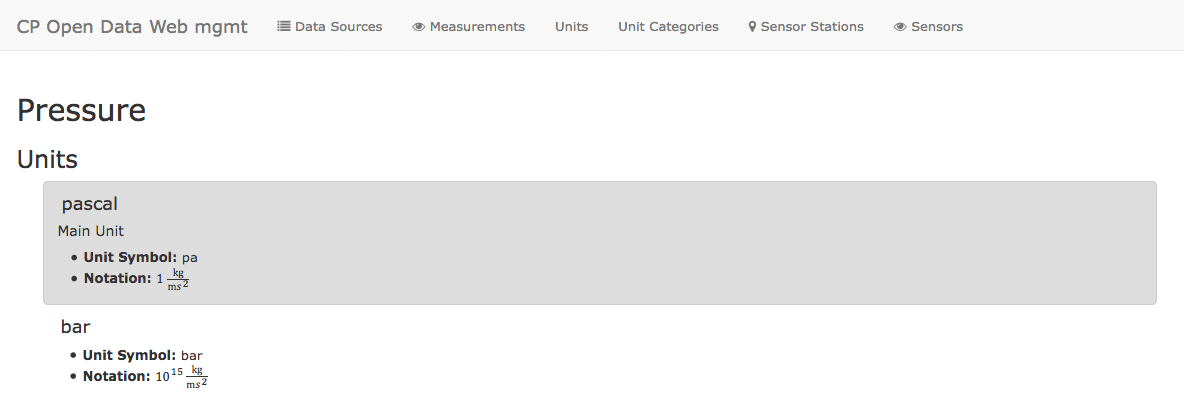
\includegraphics[width=1.00\textwidth]{images/unit_frontend.png}
	\caption{Screenshot of the units of a unit category on the web management platform. You can see the main unit and have a notation on what the units express.}
	\label{fig:screen-units}
\end{figure}

\begin{verbatim}
GET /unit_categories/:id/getMainUnit
\end{verbatim}

Example request:

\begin{verbatim}
GET /unit_categories/temperature/getMainUnit

{
    "id":"temperature_celsius",
    "name":"celsius",
    "unit_category_id":"temperature",
    "unit_symbol":"°C"
}
\end{verbatim}

\begin{verbatim}
GET /unit_categories/:id/units
\end{verbatim}

Example request:

\begin{verbatim}
GET /unit_categories/temperature/units

[
   {
      "attributes":{
         "id":"temperature_celsius",
         "name":"celsius",
         "unit_symbol":"°C",
         "unit_category_id":"temperature",
         "notation":""
      }
   },
   {
      "attributes":{
         "id":"temperature_fahrenheit",
         "name":"fahrenheit",
         "unit_symbol":"°F",
         "unit_category_id":"temperature",
         "notation":""
      }
   },
   {
      "attributes":{
         "id":"temperature_kelvin",
         "name":"kelvin",
         "unit_symbol":"K",
         "unit_category_id":"temperature",
         "notation":""
      }
   },
   ...
]
\end{verbatim}

\subsection{Discussion}\label{discussion}

As mentioned before, the planning of the extent of the functionality
offered by this system, was very vague. Besides managing metadata and
providing an API for other components, further features were at least
considered to be part of this system, like for example a scheduler that
triggers the component that handles the deployment of importers.
Therefore we chose to build this system on top of an infrastructure that
can be easily extended in many directions and has nice-to-use database
adapters instead of a more lightweight system.

While initially we also wanted to model a data source with its sensors
grouped in sensor stations, this approach would bring immense overhead
for configuring data sources in our system upfront, as a user would have
to very exactly model a data source with all its sensors and sensor
stations first. For big services like e.g.~the German Weather Service
this would be an enormous amount of work. Gathering this information
would better be done by scraping the information present in
Elasticsearch and translating them to geolocated information for all
sensors/sensor-stations/datasources. In the UML Class Diagram you can
see the modeling for this approach greyed out.

The main metainformation about the data sources (besides metadata about
the source itself) that we still needed within our system (the location
of the sensor and the grouping of sensor stations is not essential for
our system to work) and had to offer to the user registering a source
were then:

\begin{itemize}
\tightlist
\item
  Information about the measurands offered by the data source
\item
  Information about the main unit used for a measurand (see section Unit
  system)
\end{itemize}

\subsubsection{Future Improvements}\label{future-improvements}

\paragraph{Caching}

There is currently no caching solution implemented since the workloads
during development phase were quite manageable. Also including a
distributed caching system in our production pipeline seemed to be too
high of an effort and would take up significant resources that would
actually not be needed during development. We wanted, therefore, to use
the limited and expensive resources we had for actual importing.

As the number of data importers grows in production, however, requests
to the relational database would increase accordingly. Whereas scaling
the database would allow us to avoid the bottleneck, adding a cache in
front of the database to serve read requests would be sufficient to
ensure performance without incurring the cost and added complexity of
scaling. An important consideration, of course, is the frequency with
which data is updated (in our case low to none), thus making it a
perfect candidate for caching. As a distributed caching system where
read requests are very fast and possible on all nodes, Redis would be a
good fit for this use case. Writing is quite expensive due to the
replication method used by Redis, but because of the infrequent updates
to our data, we are willing to accept the trade-off in exchange for very
fast reads.

\paragraph{Exchange Scheduling information}

Due to not quite being able to reach every goal of our initial plan as
to how the architecture should look like, the scheduler had to move to
the deployment component (i.e.~the deployment to the Kubernetes
cluster). While this component should be responsible for deploying data
importers, the information about the schedule should actually be
provided to the web management system by the user. This is currently not
happening. There would be several ways how to manage scheduling and/or
deliver the scheduling information from this system to the component
handling the scheduling.

\begin{itemize}
\tightlist
\item
  Having a background processing component that acts as a scheduler
  within the web management platform. This would require an API to
  trigger the deploy on the component responsible for that, which we
  were not able to achieve.
\item
  Having a microservice-like component that is only responsible for
  scheduling and triggering importers to be deployed. This would as well
  require an API on the deployment component.
\item
  Leave the scheduling within the deployment component. This would also
  require an API, but just for receiving the general schedule, not for
  offering a hook to trigger an import.
\end{itemize}

The second option seems more granular and conforms better to our general
microservice approach but would also require the most configuration and
deployment effort. Including a scheduler in the web management platform
would somehow violate this approach but still make sense, as this
component could easily be integrated within Ruby on Rails and would be a
standalone component within it.

%\section{Data Source Metadata Management System}\label{sec:metadata}

\textbf{Authoriship: } Written by Paul Wille\\
\emph{Proofread \& edited by Andres} \\

\vspace*{4mm}

In this chapter we will discuss the component responsible for managing
metadata about the data sources which are imported to the system. We
will cover what it is and does, some thoughts around why we decided to
include such a component, and how it was realized and implemented.

\subsection{Requirements}\label{requirements}

The main purpose of the component is to:

\begin{itemize}
\tightlist
\item
  serve as a registry of data sources in the system,
\item
  provide data source metadata to other components in the system,
\item
  provide users with information about units of measurement,
\item
  enable users who want to use the data to see the resources our system
  contains
\end{itemize}

In contrast to nearly every other component we had to implement, the
management platform did not have to meet as many criteria as a
distributed cloud system in general. The data it contains is quite
static and the number of requests that we expect is also quite low.
However, the following general cloud-specific architectural style
requirements were taken into consideration:

\begin{itemize}
\tightlist
\item
  Availability to other system components, that require the held
  information
\item
  Quick response time (for query optimization within the public search
  API)
\item
  Ability to run asynchronous background tasks (for scheduling)
\end{itemize}

\subsection{Implementation}\label{implementation}

The system was built using \emph{Ruby on Rails} with \emph{PostgreSQL}
as a database. The reasons why we chose to use Rails are:

\begin{itemize}
\tightlist
\item
  Relatively fast development of an MVC web application
\item
  Well established (over a decade), has therefore lots of resources ---
  also for all kinds of extensions
\item
  Extensive community support
\item
  Very good integrated ORM adapters that could easily be exchanged for
  ODM adapters for document databases
\item
  Offers the dynamic of Ruby as programming language
\end{itemize}

\subsection{Domain Model}\label{domain-model}

\begin{figure}
	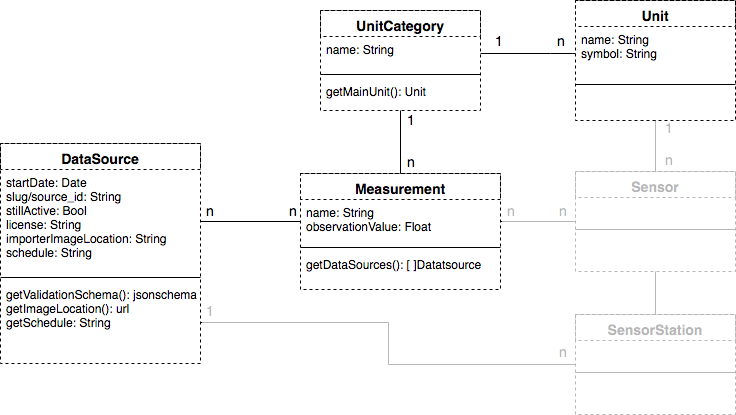
\includegraphics[width=1.00\textwidth]{images/relational_schema.png}
	\caption{UML Class Diagram of the Metadata Management System}
	\label{fig:uml-model}
\end{figure}

\subsubsection{Data Sources Registry}\label{data-sources-registry}

Before data from a given source can be imported, important information
about the source must be made available to our system. This information
consists of static metainformation and has no direct relation to actual
data being provided in the source.

We chose not to store it in the same database as the actual sensor
measurement data, but have a separate system instead. This provides
isolation between our sources and the database, preventing changes in
the choice of database or its schema from having any effect in how we
store and maintain data sources.

The metainformation that has to be provided to our system prior to
importing mainly consists of:

\begin{itemize}
\tightlist
\item
  Name of the source
\item
  Start date from which the source provides data
\item
  Whether the source is still active (i.e.~data is actively being
  provided by the source).
\item
  if not, the end date (last date for which data was provided).
\item
  Under what license the data is published
\end{itemize}

Additionally we ask the user to provide additional information, which is
useful for our system:

\begin{itemize}
\tightlist
\item
  If the data source is still active, at what schedule is new data
  published
\item
  A \emph{slug} that can be used as an id within our pipeline and in
  Elasticsearch
\item
  The measurements provided by the data source (which actual
  measurements the data source collects)
\item
  The URL location of the Docker container to be executed to import the
  data.
\end{itemize}

\begin{figure}
	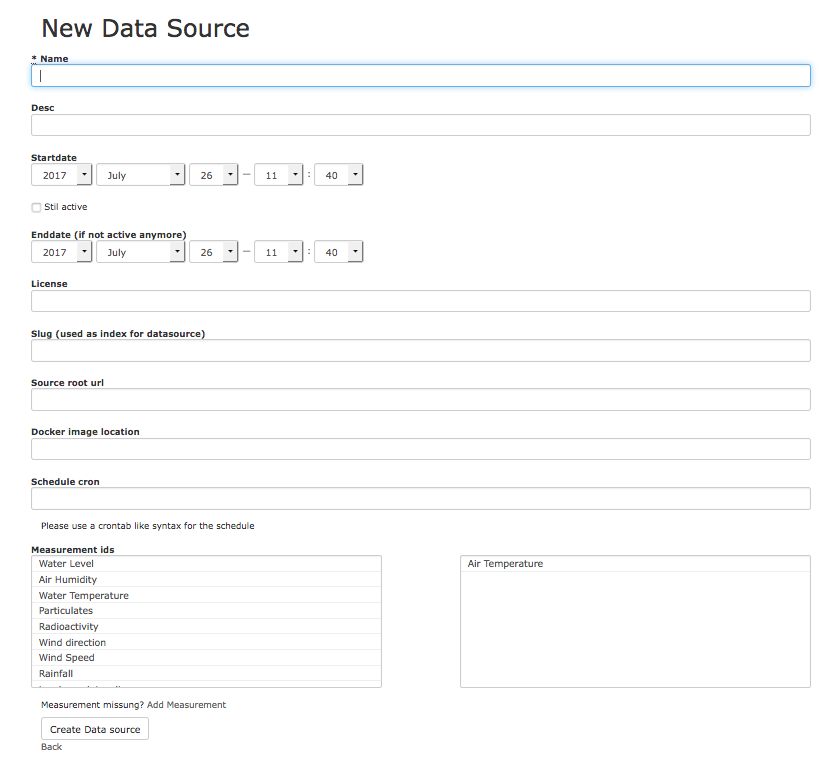
\includegraphics[width=1.00\textwidth]{images/new_datasource.png}
	\caption{Registering a data source within the Web management platform}
	\label{fig:register-source}
\end{figure}

\subsubsection{Validation Schema}\label{validation-schema}

As described in the chapter about validation and insertion into
Elasticsearch, we have a separate, distinct component that is
responsible for validating the output from data importers.

To achieve this, a schema must be provided against which to validate.
Since this schema itself is fixed, it could be hardcoded into the
validator, without the need to make another HTTP request. We decided
that this would be a bad idea for the following reasons:

\begin{itemize}
\tightlist
\item
  Sanity checks: in addition to schema-only validation, the schema
  provided by this component can validate data-source-specific values
  (such as importer IDs, etc.), which could not be validated with a
  generic validator.
\item
  Version management: schema changes over time would require changing
  the information hardcoded within the validator, and completely
  rebuilding and redeploying the validator component itself. Updating a
  record inside this component is far simpler than redeploying
  infrastructure, which is inherently more complex in an era where no
  downtime is expected.
\end{itemize}

Therefore we needed a place where said validation schema can reside. The
web management system seemed to be the right pace for that, as it
already carries metainformation about data sources and the data sources
are registered there. So it is easy to provide the relevant schema
information as well. The management system provides an API call to
supply the validation schema to the validators which looks like this:

\begin{verbatim}
GET /data_sources/:id/getValidationSchema
\end{verbatim}

The response looks like as follows (note that the const
\texttt{source\_id} would be replaced by the ID of the data source):

\begin{verbatim}
{
  "\$schema": "http://json-schema.org/schema#",
  "title": "Data Source",
  "description": "A Data Source for Open Sensor Data from the CP project \\
									at TU Berlin. ",
  "type": "object",
  "properties": {
    "source_id": {"const": "source_slug"},
    "device": {"type": "string"},
    "timestamp": { "type": "string", "format": "date-time" },
    "timestamp_data": { "type": "string", "format": "date-time" },
    "location": {
      "type": "object",
      "properties": {
        "lat": {"type": "number",
                "exclusiveMaximum": true,
                "exclusiveMinimum": true,
                "maximum": 90,
                "minimum": -90
               },
        "lon": {"type": "number",
                "exclusiveMaximum": true,
                "exclusiveMinimum": true,
                "maximum": 180,
                "minimum": -180,
               }
      },
    "required": ["lat", "lon"]
    },
    "license": {"type": "string"},
    "sensors": {
      "type": "object",
      "items": [
      {
        "type": "object",
        "properties": {
          "sensor": {"type": "string"},
          "observation_type": {"type": "string"},
          "observation_value": {"type": "number"}
        }
      }]
    }
  },
  "required": ["source_id", "timestamp","sensors", "location", "license"]
}
\end{verbatim}

\subsubsection{Provide Information to the Elasticsearch API for query
optimization}\label{provide-information-to-the-elasticsearch-api-for-query-optimization}

As described in the data model section, our model is data-source-based
and not measurand-based. For queries spanning across measurands, it will
be necessary to have further information about the relationship between
data sources and measurands.

As there were several possibilities as to where this information could
be stored and managed, and how it would be provided, the easiest place
to start with in our opinion was with the implementer of an importer,
since he or she must provide information to us when registering the data
source. The user therefore has to mark what measurements a data source
contains upfront (see Figure \ref{fig:register-source}).

In order to optimize querying, this information is provided to the API
that wraps the search interface of Elasticsearch via an API itself. The
information is stored in an indexed join table that holds the mapping
between data source and the measurands it contains. As can be seen in
the class diagram \ref{fig:uml-model} of the relational system, queries
in both directions are provided: getting all measurands for a data
source, and getting all data sources that contain a given measurand. The
corresponding routes look like this:

\begin{verbatim}
GET /data_sources/:id/measurements
\end{verbatim}

Example:

\begin{verbatim}
GET /data_sources/blume_messnetz/measurands

[
   {
      "id":1,
      "name":"Air Temperature",
      "desc":"",
      "unit_category_id":"temperature"
   },
   {
      "id":3,
      "name":"Air Humidity",
      "desc":"amount of water vapor present in the air",
      "unit_category_id":"humidity"
   }
]
\end{verbatim}

\begin{verbatim}
GET /measurements/:id/data_sources
\end{verbatim}

An example request would look like following

\begin{verbatim}
GET /measurements/1/data_sources

[
    { "id":1, "slug":"blume_messnetz", "license":"" },
    { "id":5, "slug":"german_weather_service", "license":"" }
]
\end{verbatim}

\subsubsection{Provide configuration information to the deployment
component}\label{provide-configuration-information-to-the-deployment-component}

Since the importer registration the only step in which the implementer
has to provide information to our system, it should cover all
configuration information needed to get an importer running.

\subsubsection{Units}\label{units}

With the requirements in mind, we modeled units like so:

\begin{enumerate}
\def\labelenumi{\arabic{enumi}.}
\tightlist
\item
  \textbf{Unit Categories}: Units themselves belong to a unit category.
  The unit category describes an entity for which measurements exist,
  which express their observations with one of the units of that
  category (see Figure \ref{fig:uml-model}).
\item
  Each unit has a \textbf{main unit} that we decide on. By calling the
  API or visiting the management platform a user can see, which the main
  unit is. Within our datastore we only use the main unit of a unit
  category for expressing measurements.
\item
  Units are managed by admins receptively users with permit to do so.
\item
  We therefore have a curated list of the unit categories and units
\item
  If there are units, measurements or even categories missing, each user
  can propose new ones. This proposals are also managed by the group of
  people managing the units.
\end{enumerate}

Measurements are controlled on the platform itself to allow users to
better propose new measurements, as this may happen more often. Units
and the Unit categories however are managed in a \emph{.yml} file. The
syntax we used looks like following for one entry:

\begin{verbatim}
From config/constants/units.yml:

pascal:
  id: pressure_pascal
  name: "pascal"
  unit_symbol: "pa"
  unit_category_id: pressure
  notation: "1 <centerdot>
              <mfrac>
                <mrow>
                  kg
                </mrow>
                <mrow>
                  m
                  <msup>
                          <mi>s</mi>
                          <mn>2</mn>
                </mrow>
              </mfrac>"

From config/constants/unit_categories.yml:

pressure:
  id: pressure
  name: Pressure
\end{verbatim}

The unit categories are pretty straightforward. For a unit there are
some more possibilities. Besides declaring the unit symbol, the category
it belongs to, its name you are allowed to use MathML to express what
the meaning of a unit is. This is especially helpful with units that can
be directly converted to each other (Figure \ref{fig:screen-units}).

The API of the web management system also provides calls to a) receive
the main unit of a unit category and to b) get a list of all units there
are for a unit category. Both of these information are of course aswell
accessible from the frontend of the system.

\begin{figure}[b]
	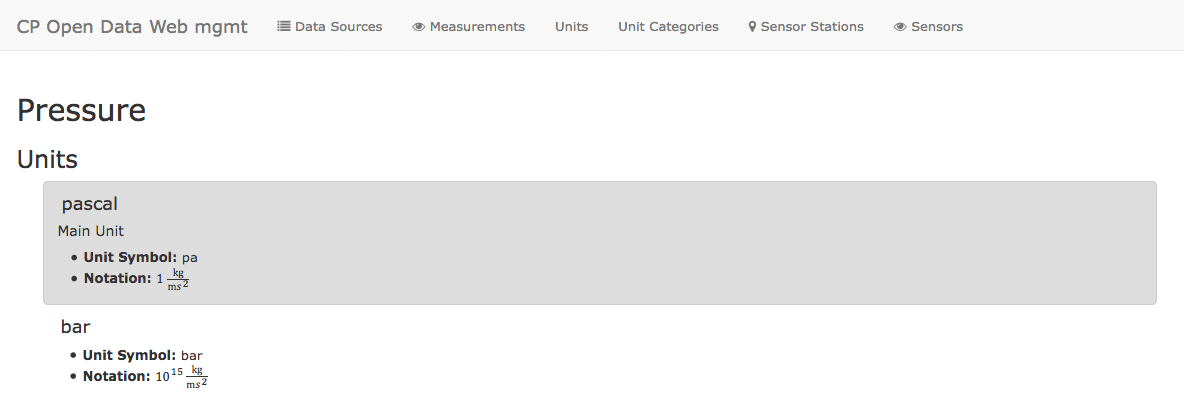
\includegraphics[width=1.00\textwidth]{images/unit_frontend.png}
	\caption{Screenshot of the units of a unit category on the web management platform. You can see the main unit and have a notation on what the units express.}
	\label{fig:screen-units}
\end{figure}

\begin{verbatim}
GET /unit_categories/:id/getMainUnit
\end{verbatim}

Example request:

\begin{verbatim}
GET /unit_categories/temperature/getMainUnit

{
    "id":"temperature_celsius",
    "name":"celsius",
    "unit_category_id":"temperature",
    "unit_symbol":"°C"
}
\end{verbatim}

\begin{verbatim}
GET /unit_categories/:id/units
\end{verbatim}

Example request:

\begin{verbatim}
GET /unit_categories/temperature/units

[
   {
      "attributes":{
         "id":"temperature_celsius",
         "name":"celsius",
         "unit_symbol":"°C",
         "unit_category_id":"temperature",
         "notation":""
      }
   },
   {
      "attributes":{
         "id":"temperature_fahrenheit",
         "name":"fahrenheit",
         "unit_symbol":"°F",
         "unit_category_id":"temperature",
         "notation":""
      }
   },
   {
      "attributes":{
         "id":"temperature_kelvin",
         "name":"kelvin",
         "unit_symbol":"K",
         "unit_category_id":"temperature",
         "notation":""
      }
   },
   ...
]
\end{verbatim}

\subsection{Discussion}\label{discussion}

As mentioned before, the planning of the extent of the functionality
offered by this system, was very vague. Besides managing metadata and
providing an API for other components, further features were at least
considered to be part of this system, like for example a scheduler that
triggers the component that handles the deployment of importers.
Therefore we chose to build this system on top of an infrastructure that
can be easily extended in many directions and has nice-to-use database
adapters instead of a more lightweight system.

While initially we also wanted to model a data source with its sensors
grouped in sensor stations, this approach would bring immense overhead
for configuring data sources in our system upfront, as a user would have
to very exactly model a data source with all its sensors and sensor
stations first. For big services like e.g.~the German Weather Service
this would be an enormous amount of work. Gathering this information
would better be done by scraping the information present in
Elasticsearch and translating them to geolocated information for all
sensors/sensor-stations/datasources. In the UML Class Diagram you can
see the modeling for this approach greyed out.

The main metainformation about the data sources (besides metadata about
the source itself) that we still needed within our system (the location
of the sensor and the grouping of sensor stations is not essential for
our system to work) and had to offer to the user registering a source
were then:

\begin{itemize}
\tightlist
\item
  Information about the measurands offered by the data source
\item
  Information about the main unit used for a measurand (see section Unit
  system)
\end{itemize}

\subsubsection{Future Improvements}\label{future-improvements}

\paragraph{Caching}

There is currently no caching solution implemented since the workloads
during development phase were quite manageable. Also including a
distributed caching system in our production pipeline seemed to be too
high of an effort and would take up significant resources that would
actually not be needed during development. We wanted, therefore, to use
the limited and expensive resources we had for actual importing.

As the number of data importers grows in production, however, requests
to the relational database would increase accordingly. Whereas scaling
the database would allow us to avoid the bottleneck, adding a cache in
front of the database to serve read requests would be sufficient to
ensure performance without incurring the cost and added complexity of
scaling. An important consideration, of course, is the frequency with
which data is updated (in our case low to none), thus making it a
perfect candidate for caching. As a distributed caching system where
read requests are very fast and possible on all nodes, Redis would be a
good fit for this use case. Writing is quite expensive due to the
replication method used by Redis, but because of the infrequent updates
to our data, we are willing to accept the trade-off in exchange for very
fast reads.

\paragraph{Exchange Scheduling information}

Due to not quite being able to reach every goal of our initial plan as
to how the architecture should look like, the scheduler had to move to
the deployment component (i.e.~the deployment to the Kubernetes
cluster). While this component should be responsible for deploying data
importers, the information about the schedule should actually be
provided to the web management system by the user. This is currently not
happening. There would be several ways how to manage scheduling and/or
deliver the scheduling information from this system to the component
handling the scheduling.

\begin{itemize}
\tightlist
\item
  Having a background processing component that acts as a scheduler
  within the web management platform. This would require an API to
  trigger the deploy on the component responsible for that, which we
  were not able to achieve.
\item
  Having a microservice-like component that is only responsible for
  scheduling and triggering importers to be deployed. This would as well
  require an API on the deployment component.
\item
  Leave the scheduling within the deployment component. This would also
  require an API, but just for receiving the general schedule, not for
  offering a hook to trigger an import.
\end{itemize}

The second option seems more granular and conforms better to our general
microservice approach but would also require the most configuration and
deployment effort. Including a scheduler in the web management platform
would somehow violate this approach but still make sense, as this
component could easily be integrated within Ruby on Rails and would be a
standalone component within it.

\section{Data Source Metadata Management System}\label{sec:metadata}

\textbf{Authoriship: } Written by Paul Wille\\
\emph{Proofread \& edited by Andres} \\

\vspace*{4mm}

In this chapter we will discuss the component responsible for managing
metadata about the data sources which are imported to the system. We
will cover what it is and does, some thoughts around why we decided to
include such a component, and how it was realized and implemented.

\subsection{Requirements}\label{requirements}

The main purpose of the component is to:

\begin{itemize}
\tightlist
\item
  serve as a registry of data sources in the system,
\item
  provide data source metadata to other components in the system,
\item
  provide users with information about units of measurement,
\item
  enable users who want to use the data to see the resources our system
  contains
\end{itemize}

In contrast to nearly every other component we had to implement, the
management platform did not have to meet as many criteria as a
distributed cloud system in general. The data it contains is quite
static and the number of requests that we expect is also quite low.
However, the following general cloud-specific architectural style
requirements were taken into consideration:

\begin{itemize}
\tightlist
\item
  Availability to other system components, that require the held
  information
\item
  Quick response time (for query optimization within the public search
  API)
\item
  Ability to run asynchronous background tasks (for scheduling)
\end{itemize}

\subsection{Implementation}\label{implementation}

The system was built using \emph{Ruby on Rails} with \emph{PostgreSQL}
as a database. The reasons why we chose to use Rails are:

\begin{itemize}
\tightlist
\item
  Relatively fast development of an MVC web application
\item
  Well established (over a decade), has therefore lots of resources ---
  also for all kinds of extensions
\item
  Extensive community support
\item
  Very good integrated ORM adapters that could easily be exchanged for
  ODM adapters for document databases
\item
  Offers the dynamic of Ruby as programming language
\end{itemize}

\subsection{Domain Model}\label{domain-model}

\begin{figure}
	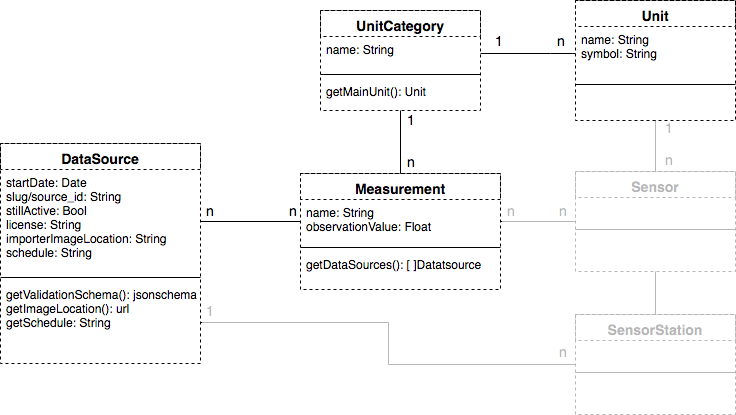
\includegraphics[width=1.00\textwidth]{images/relational_schema.png}
	\caption{UML Class Diagram of the Metadata Management System}
	\label{fig:uml-model}
\end{figure}

\subsubsection{Data Sources Registry}\label{data-sources-registry}

Before data from a given source can be imported, important information
about the source must be made available to our system. This information
consists of static metainformation and has no direct relation to actual
data being provided in the source.

We chose not to store it in the same database as the actual sensor
measurement data, but have a separate system instead. This provides
isolation between our sources and the database, preventing changes in
the choice of database or its schema from having any effect in how we
store and maintain data sources.

The metainformation that has to be provided to our system prior to
importing mainly consists of:

\begin{itemize}
\tightlist
\item
  Name of the source
\item
  Start date from which the source provides data
\item
  Whether the source is still active (i.e.~data is actively being
  provided by the source).
\item
  if not, the end date (last date for which data was provided).
\item
  Under what license the data is published
\end{itemize}

Additionally we ask the user to provide additional information, which is
useful for our system:

\begin{itemize}
\tightlist
\item
  If the data source is still active, at what schedule is new data
  published
\item
  A \emph{slug} that can be used as an id within our pipeline and in
  Elasticsearch
\item
  The measurements provided by the data source (which actual
  measurements the data source collects)
\item
  The URL location of the Docker container to be executed to import the
  data.
\end{itemize}

\begin{figure}
	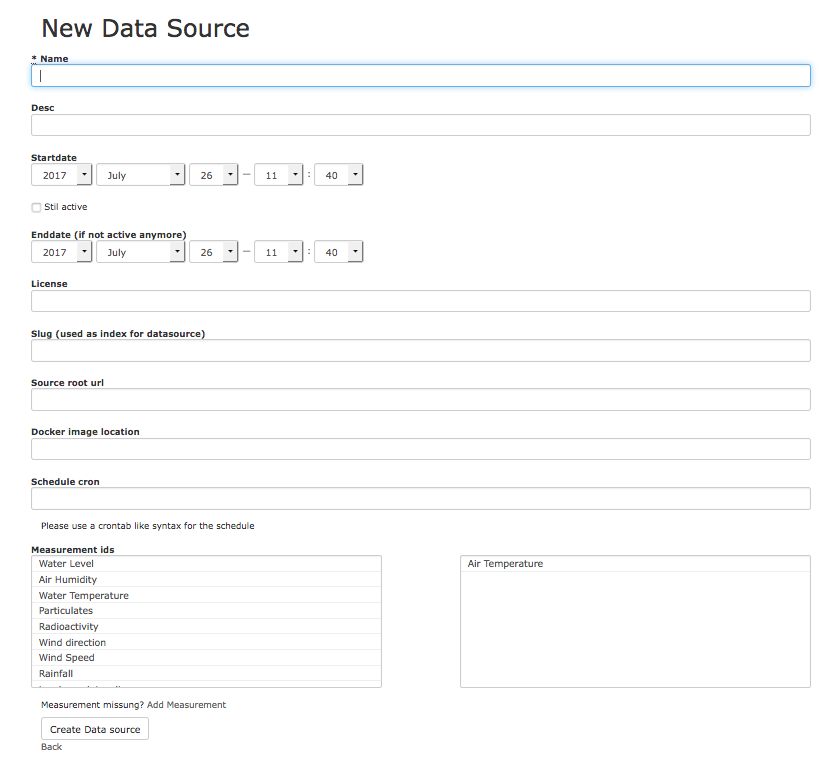
\includegraphics[width=1.00\textwidth]{images/new_datasource.png}
	\caption{Registering a data source within the Web management platform}
	\label{fig:register-source}
\end{figure}

\subsubsection{Validation Schema}\label{validation-schema}

As described in the chapter about validation and insertion into
Elasticsearch, we have a separate, distinct component that is
responsible for validating the output from data importers.

To achieve this, a schema must be provided against which to validate.
Since this schema itself is fixed, it could be hardcoded into the
validator, without the need to make another HTTP request. We decided
that this would be a bad idea for the following reasons:

\begin{itemize}
\tightlist
\item
  Sanity checks: in addition to schema-only validation, the schema
  provided by this component can validate data-source-specific values
  (such as importer IDs, etc.), which could not be validated with a
  generic validator.
\item
  Version management: schema changes over time would require changing
  the information hardcoded within the validator, and completely
  rebuilding and redeploying the validator component itself. Updating a
  record inside this component is far simpler than redeploying
  infrastructure, which is inherently more complex in an era where no
  downtime is expected.
\end{itemize}

Therefore we needed a place where said validation schema can reside. The
web management system seemed to be the right pace for that, as it
already carries metainformation about data sources and the data sources
are registered there. So it is easy to provide the relevant schema
information as well. The management system provides an API call to
supply the validation schema to the validators which looks like this:

\begin{verbatim}
GET /data_sources/:id/getValidationSchema
\end{verbatim}

The response looks like as follows (note that the const
\texttt{source\_id} would be replaced by the ID of the data source):

\begin{verbatim}
{
  "\$schema": "http://json-schema.org/schema#",
  "title": "Data Source",
  "description": "A Data Source for Open Sensor Data from the CP project \\
									at TU Berlin. ",
  "type": "object",
  "properties": {
    "source_id": {"const": "source_slug"},
    "device": {"type": "string"},
    "timestamp": { "type": "string", "format": "date-time" },
    "timestamp_data": { "type": "string", "format": "date-time" },
    "location": {
      "type": "object",
      "properties": {
        "lat": {"type": "number",
                "exclusiveMaximum": true,
                "exclusiveMinimum": true,
                "maximum": 90,
                "minimum": -90
               },
        "lon": {"type": "number",
                "exclusiveMaximum": true,
                "exclusiveMinimum": true,
                "maximum": 180,
                "minimum": -180,
               }
      },
    "required": ["lat", "lon"]
    },
    "license": {"type": "string"},
    "sensors": {
      "type": "object",
      "items": [
      {
        "type": "object",
        "properties": {
          "sensor": {"type": "string"},
          "observation_type": {"type": "string"},
          "observation_value": {"type": "number"}
        }
      }]
    }
  },
  "required": ["source_id", "timestamp","sensors", "location", "license"]
}
\end{verbatim}

\subsubsection{Provide Information to the Elasticsearch API for query
optimization}\label{provide-information-to-the-elasticsearch-api-for-query-optimization}

As described in the data model section, our model is data-source-based
and not measurand-based. For queries spanning across measurands, it will
be necessary to have further information about the relationship between
data sources and measurands.

As there were several possibilities as to where this information could
be stored and managed, and how it would be provided, the easiest place
to start with in our opinion was with the implementer of an importer,
since he or she must provide information to us when registering the data
source. The user therefore has to mark what measurements a data source
contains upfront (see Figure \ref{fig:register-source}).

In order to optimize querying, this information is provided to the API
that wraps the search interface of Elasticsearch via an API itself. The
information is stored in an indexed join table that holds the mapping
between data source and the measurands it contains. As can be seen in
the class diagram \ref{fig:uml-model} of the relational system, queries
in both directions are provided: getting all measurands for a data
source, and getting all data sources that contain a given measurand. The
corresponding routes look like this:

\begin{verbatim}
GET /data_sources/:id/measurements
\end{verbatim}

Example:

\begin{verbatim}
GET /data_sources/blume_messnetz/measurands

[
   {
      "id":1,
      "name":"Air Temperature",
      "desc":"",
      "unit_category_id":"temperature"
   },
   {
      "id":3,
      "name":"Air Humidity",
      "desc":"amount of water vapor present in the air",
      "unit_category_id":"humidity"
   }
]
\end{verbatim}

\begin{verbatim}
GET /measurements/:id/data_sources
\end{verbatim}

An example request would look like following

\begin{verbatim}
GET /measurements/1/data_sources

[
    { "id":1, "slug":"blume_messnetz", "license":"" },
    { "id":5, "slug":"german_weather_service", "license":"" }
]
\end{verbatim}

\subsubsection{Provide configuration information to the deployment
component}\label{provide-configuration-information-to-the-deployment-component}

Since the importer registration the only step in which the implementer
has to provide information to our system, it should cover all
configuration information needed to get an importer running.

\subsubsection{Units}\label{units}

With the requirements in mind, we modeled units like so:

\begin{enumerate}
\def\labelenumi{\arabic{enumi}.}
\tightlist
\item
  \textbf{Unit Categories}: Units themselves belong to a unit category.
  The unit category describes an entity for which measurements exist,
  which express their observations with one of the units of that
  category (see Figure \ref{fig:uml-model}).
\item
  Each unit has a \textbf{main unit} that we decide on. By calling the
  API or visiting the management platform a user can see, which the main
  unit is. Within our datastore we only use the main unit of a unit
  category for expressing measurements.
\item
  Units are managed by admins receptively users with permit to do so.
\item
  We therefore have a curated list of the unit categories and units
\item
  If there are units, measurements or even categories missing, each user
  can propose new ones. This proposals are also managed by the group of
  people managing the units.
\end{enumerate}

Measurements are controlled on the platform itself to allow users to
better propose new measurements, as this may happen more often. Units
and the Unit categories however are managed in a \emph{.yml} file. The
syntax we used looks like following for one entry:

\begin{verbatim}
From config/constants/units.yml:

pascal:
  id: pressure_pascal
  name: "pascal"
  unit_symbol: "pa"
  unit_category_id: pressure
  notation: "1 <centerdot>
              <mfrac>
                <mrow>
                  kg
                </mrow>
                <mrow>
                  m
                  <msup>
                          <mi>s</mi>
                          <mn>2</mn>
                </mrow>
              </mfrac>"

From config/constants/unit_categories.yml:

pressure:
  id: pressure
  name: Pressure
\end{verbatim}

The unit categories are pretty straightforward. For a unit there are
some more possibilities. Besides declaring the unit symbol, the category
it belongs to, its name you are allowed to use MathML to express what
the meaning of a unit is. This is especially helpful with units that can
be directly converted to each other (Figure \ref{fig:screen-units}).

The API of the web management system also provides calls to a) receive
the main unit of a unit category and to b) get a list of all units there
are for a unit category. Both of these information are of course aswell
accessible from the frontend of the system.

\begin{figure}[b]
	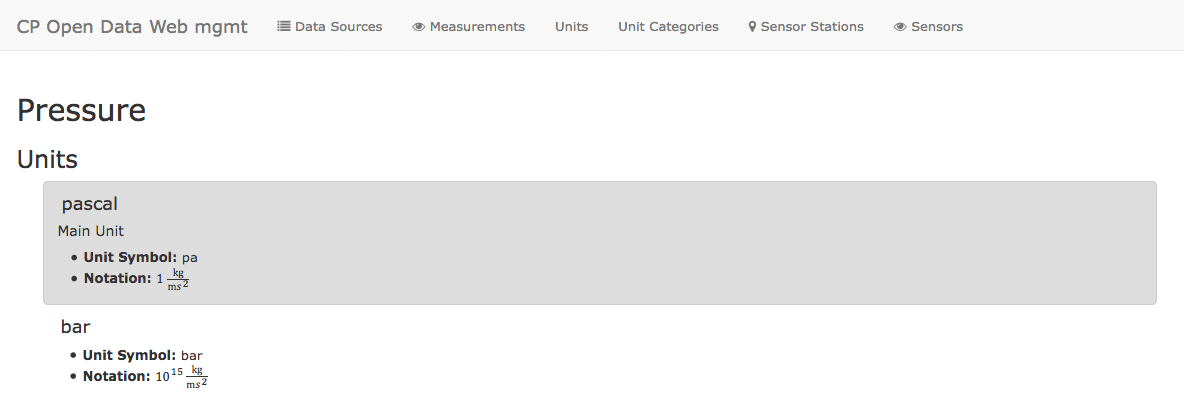
\includegraphics[width=1.00\textwidth]{images/unit_frontend.png}
	\caption{Screenshot of the units of a unit category on the web management platform. You can see the main unit and have a notation on what the units express.}
	\label{fig:screen-units}
\end{figure}

\begin{verbatim}
GET /unit_categories/:id/getMainUnit
\end{verbatim}

Example request:

\begin{verbatim}
GET /unit_categories/temperature/getMainUnit

{
    "id":"temperature_celsius",
    "name":"celsius",
    "unit_category_id":"temperature",
    "unit_symbol":"°C"
}
\end{verbatim}

\begin{verbatim}
GET /unit_categories/:id/units
\end{verbatim}

Example request:

\begin{verbatim}
GET /unit_categories/temperature/units

[
   {
      "attributes":{
         "id":"temperature_celsius",
         "name":"celsius",
         "unit_symbol":"°C",
         "unit_category_id":"temperature",
         "notation":""
      }
   },
   {
      "attributes":{
         "id":"temperature_fahrenheit",
         "name":"fahrenheit",
         "unit_symbol":"°F",
         "unit_category_id":"temperature",
         "notation":""
      }
   },
   {
      "attributes":{
         "id":"temperature_kelvin",
         "name":"kelvin",
         "unit_symbol":"K",
         "unit_category_id":"temperature",
         "notation":""
      }
   },
   ...
]
\end{verbatim}

\subsection{Discussion}\label{discussion}

As mentioned before, the planning of the extent of the functionality
offered by this system, was very vague. Besides managing metadata and
providing an API for other components, further features were at least
considered to be part of this system, like for example a scheduler that
triggers the component that handles the deployment of importers.
Therefore we chose to build this system on top of an infrastructure that
can be easily extended in many directions and has nice-to-use database
adapters instead of a more lightweight system.

While initially we also wanted to model a data source with its sensors
grouped in sensor stations, this approach would bring immense overhead
for configuring data sources in our system upfront, as a user would have
to very exactly model a data source with all its sensors and sensor
stations first. For big services like e.g.~the German Weather Service
this would be an enormous amount of work. Gathering this information
would better be done by scraping the information present in
Elasticsearch and translating them to geolocated information for all
sensors/sensor-stations/datasources. In the UML Class Diagram you can
see the modeling for this approach greyed out.

The main metainformation about the data sources (besides metadata about
the source itself) that we still needed within our system (the location
of the sensor and the grouping of sensor stations is not essential for
our system to work) and had to offer to the user registering a source
were then:

\begin{itemize}
\tightlist
\item
  Information about the measurands offered by the data source
\item
  Information about the main unit used for a measurand (see section Unit
  system)
\end{itemize}

\subsubsection{Future Improvements}\label{future-improvements}

\paragraph{Caching}

There is currently no caching solution implemented since the workloads
during development phase were quite manageable. Also including a
distributed caching system in our production pipeline seemed to be too
high of an effort and would take up significant resources that would
actually not be needed during development. We wanted, therefore, to use
the limited and expensive resources we had for actual importing.

As the number of data importers grows in production, however, requests
to the relational database would increase accordingly. Whereas scaling
the database would allow us to avoid the bottleneck, adding a cache in
front of the database to serve read requests would be sufficient to
ensure performance without incurring the cost and added complexity of
scaling. An important consideration, of course, is the frequency with
which data is updated (in our case low to none), thus making it a
perfect candidate for caching. As a distributed caching system where
read requests are very fast and possible on all nodes, Redis would be a
good fit for this use case. Writing is quite expensive due to the
replication method used by Redis, but because of the infrequent updates
to our data, we are willing to accept the trade-off in exchange for very
fast reads.

\paragraph{Exchange Scheduling information}

Due to not quite being able to reach every goal of our initial plan as
to how the architecture should look like, the scheduler had to move to
the deployment component (i.e.~the deployment to the Kubernetes
cluster). While this component should be responsible for deploying data
importers, the information about the schedule should actually be
provided to the web management system by the user. This is currently not
happening. There would be several ways how to manage scheduling and/or
deliver the scheduling information from this system to the component
handling the scheduling.

\begin{itemize}
\tightlist
\item
  Having a background processing component that acts as a scheduler
  within the web management platform. This would require an API to
  trigger the deploy on the component responsible for that, which we
  were not able to achieve.
\item
  Having a microservice-like component that is only responsible for
  scheduling and triggering importers to be deployed. This would as well
  require an API on the deployment component.
\item
  Leave the scheduling within the deployment component. This would also
  require an API, but just for receiving the general schedule, not for
  offering a hook to trigger an import.
\end{itemize}

The second option seems more granular and conforms better to our general
microservice approach but would also require the most configuration and
deployment effort. Including a scheduler in the web management platform
would somehow violate this approach but still make sense, as this
component could easily be integrated within Ruby on Rails and would be a
standalone component within it.


\begin{thebibliography}{}  % (do not forget {}) and Put your bib.txt in here

%\bibitem[1982]{database:example}
Clarke, F., Ekeland, I.:
Nonlinear oscillations and boundary-value problems for
Hamiltonian systems.
Arch. Rat. Mech. Anal. 78, 315--333 (1982)

%\bibitem[1982]{database:example}
Clarke, F., Ekeland, I.:
Nonlinear oscillations and boundary-value problems for
Hamiltonian systems.
Arch. Rat. Mech. Anal. 78, 315--333 (1982)


\appendix

\section{Imported Data Sources}

\begin{table}[]
\centering
\caption{Data Sources}
\label{data_sources}
\begin{tabular}{llllll}
 No. & Name  & Description & Measurand & Supported Data Format & URL \\
 1 & Weather Data Stuttgart & The source is part of the \textbf{OK Lab Stuttgart} project which includes 300 fine dust sensors. & Humidity, Temperature, Pressure &csv & luftdaten.info \\
 2 & Luftdaten Brandenburg & Air quality data from 28 data measuring stations in Brandenburg, Germany. & O₃, NO, NO₂, PM10, PM2.5, SO₂, CO & xls & luftdaten.brandenburg.de \\
 3 & Umweltbundesamt & Current air quality data from about 500 data measuring stations for 16 states and cities of Germany. & PM10, SO₂, O₃, NO₂, CO & csv &  umweltbundesamt.de \\
 4 & Pegel Online Water Level & Raw values of \textbf{Water Level} for internal and coastal levels of waterways of the Germany up to a maximum of 30 days & Water Level & REST, SOAP, HTTP & pegelonline.wsv.de \\
 5 & BLUME &  & Stickoxide, Schwefeldioxid, Schwebstaub (PM10), Benzol, Kohlenmonoxid und Ozon & HTML & http://www.berlin.de/senuvk/umwelt/luftqualitaet/de/messnetz/aktuelle_werte.shtml \\
 6 & BFS UV-Index &  & UV-Index & HTML & http://www.bfs.de/DE/themen/opt/uv/uv-index/aktuell/aktuell_node.html
\end{tabular}
\end{table}


\end{thebibliography}

\end{document}
